% !TEX program = xelatex
\documentclass[a4paper]{article}
\usepackage[UTF8]{ctex}
\setCJKmainfont{SimSun}[BoldFont=SimHei,ItalicFont=KaiTi]
\setCJKsansfont{SimHei}
\usepackage[top=3mm,bottom=3mm,left=4mm,right=4mm]{geometry}
\usepackage{amsmath,amssymb,bm}
\usepackage{multicol}
\usepackage{graphicx}
\usepackage{tikz}
\usetikzlibrary{arrows.meta}
\usepackage[dvipsnames]{xcolor}
\usepackage{enumitem}
\usepackage{array,tabularx}
\pagestyle{empty}
\setlength{\parindent}{0pt}
\setlength{\parskip}{0pt}
\setlength{\columnsep}{2.8mm}
\setlength{\columnseprule}{0.15pt}
\setlength{\tabcolsep}{1.0pt}
\setlength{\fboxsep}{0.8pt}
\renewcommand{\baselinestretch}{0.695}
\setlist{nosep,leftmargin=7pt,labelsep=1.5pt,itemsep=0pt,parsep=0pt,topsep=0pt}
\definecolor{h1}{HTML}{0D47A1}
\definecolor{h2}{HTML}{1565C0}
\definecolor{h3}{HTML}{E65100}
\definecolor{warnc}{HTML}{B71C1C}
\definecolor{tip}{HTML}{1B5E20}
\definecolor{bg}{HTML}{F7FAFF}
\definecolor{bgw}{HTML}{FFF3E0}
\definecolor{realc}{HTML}{B71C1C}
\definecolor{subc}{HTML}{1565C0}
\definecolor{varc}{HTML}{1B5E20}
\definecolor{idc}{HTML}{6A1B9A}
\definecolor{stepc}{HTML}{E65100}
\definecolor{formc}{HTML}{006064}
\definecolor{lookc}{HTML}{5D4037}
\definecolor{errc}{HTML}{C62828}
\definecolor{conc}{HTML}{283593}
\definecolor{symc}{HTML}{37474F}
\definecolor{quickc}{HTML}{AD1457}
\definecolor{infoc}{HTML}{00695C}
\definecolor{infobg}{HTML}{E0F2F1}
\newcommand{\chap}[1]{\vspace{0.35pt}{\fontsize{6.55}{6.78}\selectfont\bfseries\color{white}\colorbox{h1}{\strut\;#1\;}}\par\vspace{0.15pt}}
\newcommand{\tagsec}[3]{\vspace{0.10pt}{\fontsize{5.05}{5.24}\selectfont\bfseries\color{#1}\colorbox{#1}{\color{white}\fontsize{4.00}{4.14}\selectfont #2}\,#3}\par}
\newcommand{\realq}[1]{\tagsec{realc}{真题}{#1}}
\newcommand{\subq}[1]{\tagsec{subc}{子题}{#1}}
\newcommand{\varq}[1]{\tagsec{varc}{变式}{#1}}
\newcommand{\idq}[1]{\tagsec{idc}{识别}{#1}}
\newcommand{\stepq}[1]{\tagsec{stepc}{步骤}{#1}}
\newcommand{\formq}[1]{\tagsec{formc}{公式链}{#1}}
\newcommand{\lookq}[1]{\tagsec{lookc}{查表}{#1}}
\newcommand{\errq}[1]{\tagsec{errc}{易错}{#1}}
\newcommand{\conceptq}[1]{\tagsec{conc}{概念}{#1}}
\newcommand{\symq}[1]{\tagsec{symc}{符号}{#1}}
\newcommand{\quickq}[1]{\tagsec{quickc}{速算}{#1}}
\newcommand{\dbsection}[1]{\vspace{0.45pt}{\fontsize{5.8}{6.0}\selectfont\bfseries\color{white}\colorbox{infoc}{\strut\;#1\;}}\par\vspace{0.15pt}}
\newcommand{\dbblock}[1]{\par\noindent\colorbox{infobg}{\begin{minipage}{\dimexpr\linewidth-2\fboxsep\relax}\fontsize{4.85}{5.05}\selectfont #1\end{minipage}}\par\vspace{0.10pt}}
\newcommand{\infoh}[1]{\vspace{0.10pt}{\fontsize{5.05}{5.24}\selectfont\bfseries\color{white}\colorbox{infoc}{\strut\;#1\;}}\par}
\newcommand{\infotxt}[1]{\colorbox{infobg}{\begin{minipage}{\dimexpr\linewidth-2\fboxsep\relax}\fontsize{4.82}{5.02}\selectfont #1\end{minipage}}\par\vspace{0.10pt}}
\newcommand{\sect}[1]{\subq{#1}}
\newcommand{\exm}[1]{\varq{#1}}
\newcommand{\mview}[1]{\colorbox{bgw}{\begin{minipage}{\dimexpr\linewidth-2\fboxsep\relax}\fontsize{4.88}{5.04}\selectfont #1\end{minipage}}\par\vspace{0.15pt}}
\newcommand{\key}[1]{{\bfseries\color{h3}#1}}
\newcommand{\warn}[1]{{\bfseries\color{warnc}#1}}
\newsavebox{\fitbox}
\newcommand{\fitmath}[2][\dimexpr\linewidth-5pt\relax]{%
  \sbox{\fitbox}{$\displaystyle #2$}%
  \ifdim\wd\fitbox>#1
    \resizebox{#1}{!}{$\displaystyle #2$}%
  \else
    \usebox{\fitbox}%
  \fi}
% 公式可读性策略：
% 1. 短公式：仍然行内显示，但使用 \textstyle，避免小分式被显示式撑高。
% 2. 长公式：不再硬压缩成一行，自动改为独立块公式，用显示式排版。
% 3. 真正超长且必须一行塞下的公式，仍可手动用 \fitmath。
\newcommand{\smartfml}[2]{%
  \sbox{\fitbox}{$\textstyle #2$}%
  \ifdim\wd\fitbox>.72\linewidth
    \colorbox{#1}{\begin{minipage}{\dimexpr\linewidth-2\fboxsep\relax}\centering\fontsize{5.10}{5.42}\selectfont\ensuremath{\displaystyle #2}\end{minipage}}%
  \else
    \colorbox{#1}{\ensuremath{\textstyle #2}}%
  \fi}
\newcommand{\fml}[1]{\smartfml{bg}{#1}}
\newcommand{\wfml}[1]{\smartfml{bgw}{#1}}
\newcommand{\fmlb}[1]{\par\noindent\colorbox{bg}{\begin{minipage}{\dimexpr\linewidth-2\fboxsep\relax}\centering\fontsize{5.12}{5.42}\selectfont\ensuremath{\displaystyle #1}\end{minipage}}\par\vspace{0.10pt}}
\newcommand{\wfmlb}[1]{\par\noindent\colorbox{bgw}{\begin{minipage}{\dimexpr\linewidth-2\fboxsep\relax}\centering\fontsize{5.12}{5.42}\selectfont\ensuremath{\displaystyle #1}\end{minipage}}\par\vspace{0.10pt}}
\newcommand{\miniimg}[2]{\begin{center}\includegraphics[width=#1\columnwidth]{#2}\end{center}\vspace{-3pt}}
\newcommand{\schemabasics}{\begin{center}\begin{tikzpicture}[>=Latex,scale=0.58,every node/.style={font=\tiny}]
\draw[thick] (0,1.5)--(0,0)--(0.55,0)--(0.55,1.15);
\draw[thick] (1.2,1.35)--(1.2,0)--(0.65,0)--(0.65,0.95);
\draw[blue] (0.02,1.05)--(0.53,1.05) (0.67,0.82)--(1.18,0.82);
\node at (0.6,-0.25){U管/差压};
\draw[thick] (1.85,0.05)--(2.75,0.25)--(2.75,1.35)--(1.85,1.15)--cycle;
\draw[->,blue] (1.65,0.75)--(2.12,0.75);
\node at (2.35,1.55){闸门};
\draw[thick,->] (3.25,0.25)--(4.0,0.25)--(4.45,0.70);
\draw[thick] (3.25,0.45)--(3.95,0.45)--(4.30,0.80);
\draw[->,red] (3.10,0.35)--(3.45,0.35);
\draw[->,red] (4.25,0.65)--(4.58,0.98);
\node at (3.85,-0.25){弯管动量};
\draw[thick] (5.05,0.1)--(6.2,0.1);
\draw[thick,->] (5.25,0.25)--(6.05,0.25);
\node at (5.65,0.55){平板边界层};
\end{tikzpicture}\end{center}\vspace{-3pt}}
\newcommand{\schemepotential}{\begin{center}\begin{tikzpicture}[>=Latex,scale=0.58,every node/.style={font=\tiny}]
% 1. 圆柱绕流
\draw[->, gray, very thin] (-0.2,0)--(1.5,0) node[right]{$x$};
\draw[->, gray, very thin] (0.65,-0.7)--(0.65,0.7) node[above]{$y$};
\draw[blue, ->] (-0.1,0.35) .. controls (0.3,0.5) and (1.0,0.5) .. (1.4,0.35);
\draw[blue, ->] (-0.1,-0.35) .. controls (0.3,-0.5) and (1.0,-0.5) .. (1.4,-0.35);
\draw[blue, ->] (-0.1,0) -- (0.3,0);
\draw[blue, ->] (1.0,0) -- (1.4,0);
\draw[thick, fill=gray!10] (0.65,0) circle (0.3);
\node at (0.65,-0.9){圆柱绕流};

% 2. Rankine体
\draw[thick, fill=gray!10] (2.9,0) ellipse (0.75 and 0.38);
\draw[fill=red] (2.55,0) circle (0.03) node[below]{\tiny 源};
\draw[fill=blue] (3.25,0) circle (0.03) node[below]{\tiny 汇};
\node at (2.9,-0.9){Rankine卵};

% 3. 壁面镜像
\draw[thick] (4.6,-0.7)--(4.6,0.7);
\foreach \y in {-0.6,-0.4,-0.2,0,0.2,0.4,0.6}{\draw (4.6,\y)--(4.5,\y-0.1);}
\draw[fill=black] (5.15,0) circle (0.04) node[right]{涡};
\draw[fill=gray] (4.05,0) circle (0.04) node[left]{镜像};
\node at (4.6,-0.9){壁面镜像};
\end{tikzpicture}\end{center}\vspace{-3pt}}
\newcommand{\schemelaval}{\begin{center}\begin{tikzpicture}[>=Latex,scale=0.58,every node/.style={font=\tiny}]
\draw[thick] (0,0.7).. controls (1.0,0.55) and (1.2,0.25)..(2.0,0.25).. controls (2.8,0.25) and (3.0,0.65)..(4.2,0.8);
\draw[thick] (0,-0.7).. controls (1.0,-0.55) and (1.2,-0.25)..(2.0,-0.25).. controls (2.8,-0.25) and (3.0,-0.65)..(4.2,-0.8);
\draw[dashed] (2.0,-0.55)--(2.0,0.55); \node at (2.0,-0.78){喉$A^*$};
\draw[->,blue] (-0.25,0)--(0.55,0); \node at (0,1.02){$p_0,T_0$};
\node at (4.15,1.02){$p_e,p_b$}; \draw[->,blue] (3.35,0)--(4.25,0);
\draw[red,thick] (3.0,-0.55)--(3.0,0.55); \node[red] at (3.22,0.72){正激波?};
\node at (2.2,1.12){Laval喷管};
\end{tikzpicture}\end{center}\vspace{-3pt}}
\newcommand{\schemeshock}{\begin{center}\begin{tikzpicture}[>=Latex,scale=0.62,every node/.style={font=\fontsize{4.8}{5.8}\selectfont}]
% Left: Oblique Shock
\draw[thick] (0,0) -- (0.8,0) -- (2.2,0.5);
\draw[dashed, gray] (0.8,0) -- (2.2,0); % base line for angles
\draw[red, thick] (0.8,0) -- (2.0,0.9);
\node[red, above right] at (2.0,0.9) {斜激波};
\draw[->, blue, thick] (0.1,0.2) -- (0.7,0.2) node[midway, above=1pt] {$Ma_1$};
\draw[->, blue, thick] (1.4,0.36) -- (2.0,0.58) node[midway, above=1pt] {$Ma_2$};
% Angle annotations (corners at 0.8,0)
\draw[thin] (1.4,0) arc (0:20:0.6); \node at (1.55,0.10) {$\theta$};
\draw[thin] (1.7,0) arc (0:37:0.9); \node at (1.85,0.32) {$\beta$};

% Right: Expansion Fan
\draw[thick] (3.2,0) -- (4.0,0) -- (5.2,-0.5);
\draw[red, thin] (4.0,0) -- ++(0:1.1);
\draw[red, thin] (4.0,0) -- ++(-7:1.1);
\draw[red, thin] (4.0,0) -- ++(-15:1.1);
\draw[red, thin] (4.0,0) -- ++(-23:1.1);
\node[red, right] at (5.15,-0.05) {膨胀扇 $\delta$};
\draw[->, blue, thick] (3.3,0.2) -- (3.9,0.2) node[midway, above=1pt] {$Ma_1$};
\draw[->, blue, thick] (4.5,-0.2) -- (5.1,-0.42) node[midway, below left] {$Ma_2$};
\end{tikzpicture}\end{center}\vspace{-3pt}}
\newcommand{\schemeviscous}{\begin{center}\begin{tikzpicture}[>=Latex,scale=0.85,every node/.style={font=\fontsize{4.8}{5.8}\selectfont}]
% ==================== LEFT: PUMP CAVITATION ====================
% Water in pool
\fill[blue!10] (-0.3,0) rectangle (0.5,0.7);
\draw[blue, thick] (-0.3,0.7) -- (0.5,0.7);
\node[blue, above, font=\fontsize{4}{5}\selectfont] at (0.1,0.7) {水面};
% Pool wall
\draw[thick] (-0.3,1.0) -- (-0.3,0) -- (0.5,0) -- (0.5,0.4);
% Suction pipe
\draw[thick] (0.05,0.2) -- (0.05,0.95) coordinate(A) .. controls (0.05,1.15) and (0.3,1.15) .. (0.5,1.15) -- (1.3,1.15);
\draw[thick] (0.25,0.2) -- (0.25,0.85) coordinate(B) .. controls (0.25,0.95) and (0.35,0.95) .. (0.5,0.95) -- (1.3,0.95);
% Pump circle
\draw[thick, fill=white] (1.5,1.05) circle (0.22);
\node[font=\fontsize{4.5}{5.5}\selectfont] at (1.5,1.05) {泵P};
% Inflow arrow inside pool
\draw[->, blue!70, thick] (0.15,0.05) -- (0.15,0.35);
% Reference lines for h
\draw[dashed, gray, ultra thin] (-0.3,0.7) -- (2.1,0.7);
\draw[dashed, gray, ultra thin] (1.5,1.05) -- (2.1,1.05);
\draw[<->, >=Stealth, thin] (2.0,0.7) -- (2.0,1.05) node[midway, right] {$h$};
\node[below] at (0.8, -0.1) {吸水泵安装高度/汽蚀};

% ==================== RIGHT: COUETTE / POISEUILLE ====================
% Bottom plate (fixed)
\draw[line width=1pt] (3.6,0) -- (5.6,0);
\foreach \x in {3.6, 3.8, 4.0, 4.2, 4.4, 4.6, 4.8, 5.0, 5.2, 5.4, 5.6}
  \draw[ultra thin] (\x, 0) -- (\x-0.08, -0.08);
% Top plate (moving)
\draw[line width=1pt] (3.6,1.0) -- (5.6,1.0);
\foreach \x in {3.6, 3.8, 4.0, 4.2, 4.4, 4.6, 4.8, 5.0, 5.2, 5.4, 5.6}
  \draw[ultra thin] (\x, 1.0) -- (\x+0.08, 1.08);
% Wall velocity U
\draw[->, red, thick] (4.4, 1.15) -- (5.2, 1.15) node[right=1pt] {$U$};
% Reference line u=0
\draw[dashed, gray] (4.0,0) -- (4.0,1.0);
\node[below, gray] at (4.0,0) {$u=0$};
% Velocity profile (combination of linear and parabolic)
\draw[blue, thick] (4.0,0) .. controls (4.5, 0.3) and (4.8, 0.7) .. (5.0,1.0);
% Velocity vector arrows
\draw[->, blue!60, thin] (4.0, 0.2) -- (4.23, 0.2);
\draw[->, blue!60, thin] (4.0, 0.4) -- (4.45, 0.4);
\draw[->, blue!60, thin] (4.0, 0.6) -- (4.68, 0.6);
\draw[->, blue!60, thin] (4.0, 0.8) -- (4.86, 0.8);
% Labels
\draw[<->, >=Stealth, thin] (3.3,0) -- (3.3,1.0) node[midway, left] {$h$};
\node[blue, right] at (4.5, 0.45) {$u(y)$};
\node[below] at (4.6, -0.1) {Couette/Poiseuille流};
\end{tikzpicture}\end{center}\vspace{-3pt}}
\newcommand{\schemebl}{\begin{center}\begin{tikzpicture}[>=Latex,scale=0.58,every node/.style={font=\tiny}]
\draw[thick] (0,0)--(3.4,0); \draw[->,blue] (-0.2,0.55)--(0.7,0.55); \node at (0.15,0.82){$U$};
\draw[red,thick] (0,0).. controls (1.1,0.25) and (2.4,0.55)..(3.4,0.85);
\draw[dashed] (2.6,0)--(2.6,0.68); \node[right] at (2.62,0.36){$\delta(x)$};
\node at (1.65,-0.25){平板边界层};
\draw[thick] (4.1,0) circle (0.65);
\draw[red,thick] (3.45,0.18).. controls (4.0,0.7) and (4.6,0.7)..(4.95,0.18);
\draw[red,thick] (3.45,-0.18).. controls (4.0,-0.7) and (4.6,-0.7)..(4.95,-0.18);
\node at (4.1,-0.95){圆柱分离尾流};
\end{tikzpicture}\end{center}\vspace{-3pt}}
\newcommand{\pvzfig}{\par\vspace{-2pt}\noindent\hfill\begin{tikzpicture}[>=Latex,scale=0.34,every node/.style={font=\tiny},baseline=(current bounding box.center)]
\draw[thick, fill=gray!10] (0,0) -- (0,3.2) -- (1,3.2) -- (1,1.3) -- (2.8,1.3) -- (2.8,1.5) -- (5,1.5) -- (5,2.2) -- (6,2.2) -- (6,0) -- (5,0) -- (5,0.7) -- (2.8,0.7) -- (2.8,0.9) -- (1,0.9) -- (1,0) -- cycle;
\draw[blue, thick] (0.02,2.8) -- (0.98,2.8);
\draw[blue, thick] (5.02,1.8) -- (5.98,1.8);
\draw[dashed, gray] (1,1.1) -- (5,1.1);
\draw[dashed, gray] (0.5,2.8) -- (5.5,2.8);
\draw[dashed, gray] (5.0,1.8) -- (5.5,1.8);
\draw[dashed, gray] (0.5,1.1) -- (1.0,1.1);
\draw[blue, ->, thick] (1.5,1.1) -- (4.5,1.1);
\draw[<->] (0.5,1.1) -- (0.5,2.8) node[midway, left] {$H$};
\draw[<->] (5.5,1.8) -- (5.5,2.8) node[midway, right] {$h$};
\node[above] at (0.5,2.8) {C};
\node[above] at (5.5,1.8) {D};
\node[below] at (1.9,0.9) {A细};
\node[below] at (3.9,0.7) {B粗};
\node[above] at (2.8,1.5) {突扩};
\end{tikzpicture}\hfill\null\par\vspace{-3pt}}
\begin{document}
\fontsize{5.15}{5.34}\selectfont

% ==================== PAGE 1 ====================
\begin{multicols}{3}
\chap{母题1 管路机械能综合：两油箱变径突扩管15分题}
\mview{\key{母题定位}：这题足够做母题。它覆盖大水面简化、管径变化、局部损失、沿程损失、层流/湍流判定、点压强、液面差反推。看见“水池/油箱/管道/阀/弯头/突扩/泵/水轮机/粗糙度”，先归到本母题。}
\pvzfig
\idq{题干完整骨架}
两油箱液面差$h=0.5$m，左液面到管轴$H=1.0$m；前段$D_1=0.1$m，后段$D_2=0.4$m，中间突扩；入口$k_e=0.5$，出口$k_d=1.0$；油$s=0.9,\mu=0.04$。问：(a)短管忽略沿程，求$Q,p_A,p_B$；(b)长管给$Q=0.006$m$^3$/s，$L_1=50$m，$L_2=100$m，$\varepsilon=0.046$mm，求所需液面差。
\stepq{落笔流程：先液面到液面，再液面到管内点}
1 选两自由液面为总方程截面：$p=0$表压，$V\approx0$。2 管段速度分别算，不能全用一个$V$。3 局部损失用元件所在管段速度；突扩用$(V_1-V_2)^2/(2g)$。4 求管内A/B点压强时，从最近液面列到该点，保留该点速度头和中间损失。
\formq{统一公式链：PVZ加损失}
\fmlb{\begin{aligned}
z_1+\frac{p_1}{\rho g}+\alpha_1\frac{V_1^2}{2g}+H_p
&=z_2+\frac{p_2}{\rho g}+\alpha_2\frac{V_2^2}{2g}+H_T+h_L\\
h_L&=\sum_i\lambda_i\frac{L_i}{D_i}\frac{V_i^2}{2g}
+\sum_j k_j\frac{V_j^2}{2g}\\
&\quad+\sum_{\text{突扩}}\frac{(V_{\rm in}-V_{\rm out})^2}{2g}
\end{aligned}}
\subq{求流量Q：短管只算局部损失}
因$A_2=16A_1$，故$V_2=V_1/16$。两液面列PVZ：
\fmlb{\begin{aligned}
h&=k_e\frac{V_1^2}{2g}+\frac{(V_1-V_2)^2}{2g}+k_d\frac{V_2^2}{2g}\\
0.5&=\left[0.5+\left(\frac{15}{16}\right)^2+\left(\frac1{16}\right)^2\right]\frac{V_1^2}{2g}\\
V_1&=2.66{\rm m/s},\qquad Q=A_1V_1=2.09\times10^{-2}{\rm m^3/s}
\end{aligned}}
\subq{求A/B点压强：从最近液面列到管内点}
A在细管，左液面到A包含入口损失和A点速度头：
\fmlb{\begin{aligned}
H&=\frac{p_A}{\rho g}+\frac{V_1^2}{2g}+k_e\frac{V_1^2}{2g}\\
\frac{p_A}{\rho g}&=H-1.5\frac{V_1^2}{2g}=0.458{\rm m\ oil},\quad p_A\approx4.04{\rm kPa}
\end{aligned}}
B在粗管，若B到右液面只剩出口损失，则速度头与出口损失抵消成液面高差：
\fmlb{\begin{aligned}
\frac{p_B}{\rho g}&=H-h=0.50{\rm m\ oil},
&p_B&\approx4.41{\rm kPa}
\end{aligned}}
\subq{长管反推液面差：给Q/L/e，先Re再损失}
\fmlb{\begin{aligned}
V_1&=0.764,\quad V_2=0.0478\\
Re_1&=1719,\quad Re_2=430\quad(\text{均层流})\\
\lambda_1&=0.0372,\quad \lambda_2=0.149
\end{aligned}}
\fmlb{\begin{aligned}
h_e&=0.0149,\quad h_d\approx0.0001,\quad h_x=0.0261\\
h_{f1}&=0.553,\quad h_{f2}=0.0043\\
h&=\sum h_L\approx0.60{\rm m}
\end{aligned}}
\realq{圆管流动与粗糙度反推：光滑管求$Q$，粗糙管反推$\varepsilon$}
原题：$D=10$cm，$L=200$m的光滑水平圆管连接两个$20^\circ$C水槽，水位$800$m与$650$m，求$Q$；若粗糙管实际$Q=100$m$^3$/h，求平均粗糙度。\\
\stepq{解题链}
两水槽自由面：$h_L=150$m，全变沿程损失。第一问光滑湍流用Blasius；第二问由实际$Q$反算$\lambda$再反推$\varepsilon$。
\fmlb{\begin{aligned}
\text{(1) 光滑: }&
\lambda=0.3164Re^{-1/4},\quad \nu=1.005\times10^{-6}\\
V&=\left[\frac{2gD^{5/4}h_L}{0.3164L\nu^{1/4}}\right]^{4/7}
=12.46{\rm m/s}\\
Q&=V\pi D^2/4=9.79\times10^{-2}{\rm m^3/s}
\approx3.52\times10^2{\rm m^3/h}
\end{aligned}}
\fmlb{\begin{aligned}
\text{(2) 粗糙: }&
V=\frac{100/3600}{\pi(0.1)^2/4}=3.537,\quad Re=3.52\times10^5\\
\lambda&=h_L\frac{D}{L}\frac{2g}{V^2}
=150\frac{0.1}{200}\frac{2g}{3.537^2}=0.1176\\
\frac1{\sqrt\lambda}&\simeq-2\log_{10}\frac{\varepsilon}{3.7D},\quad
\varepsilon=3.7D\,10^{-1/(2\sqrt\lambda)}\approx12.9{\rm mm}
\end{aligned}}
\errq{本题检查}
光滑管不用粗糙度；$m^3$/h要除3600；反推粗糙度不是$\lambda$相减，而是$Q\to V,Re\to\lambda\to\varepsilon$。
\subq{作业代表题：离心泵吸水管最大安装高度}
原题：镀锌钢管$\varepsilon=0.15$mm，$L=6$m，$d=100$mm，弯头$\zeta=0.29$，进口阀$\zeta=2.5$，$Q=50$m$^3$/h，$p_v=19.6$kPa，$p_a=101.3$kPa，入口压至少比汽化压大20kPa，求泵中心高出水面$h_{\max}$。\\
选水面A到泵入口B，无泵项，$p_B=p_v+20=39.6$kPa\warn{绝压}：
\fmlb{\begin{aligned}
h&=\frac{p_a-p_B}{\rho g}-\frac{V^2}{2g}
-\left(\lambda\frac{L}{d}+\sum\zeta\right)\frac{V^2}{2g}\\
Q&=0.01389,\ V=Q/(\pi d^2/4)=1.77,\ Re=1.77\times10^5\\
\varepsilon/d&=0.0015,\ \lambda\simeq0.023,\ \sum\zeta=2.79\\
h&=6.29-0.159-(1.38+2.79)0.159=5.47{\rm m}
\end{aligned}}
\subq{作业代表题：水轮机输出功率}
原题：斜管$d_1=0.20$m，$L_1=30$m，$V_1=2$m/s；水平管$d_2=0.30$m，$L_2=15$m；铸铁$\varepsilon=0.25$mm，$\nu=1.3\times10^{-6}$，压表70kPa，上游水面比压表截面高30m，忽略局损，求输出功率。\\
\fmlb{\begin{aligned}
Q&=\pi d_1^2V_1/4=0.0628,\quad V_2=Q/(\pi d_2^2/4)=0.889\\
Re_1&=3.08\times10^5,\ Re_2=2.05\times10^5,\ 
\lambda_1\simeq0.0216,\lambda_2\simeq0.0203\\
h_f&=\lambda_1\frac{L_1}{d_1}\frac{V_1^2}{2g}
+\lambda_2\frac{L_2}{d_2}\frac{V_2^2}{2g}\\
&=0.700{\rm m}\\
H_T&=30-\frac{70000}{1000g}
-\frac{0.889^2}{2g}-0.700\\
&=22.12{\rm m}\\
P&=\rho gQH_T=13.6{\rm kW}
\end{aligned}}
\columnbreak
\dbsection{A. 母题1常数、单位、表压/绝压}
\dbblock{%
$g=9.81\,{\rm m/s^2}$；水$\rho=1000\,{\rm kg/m^3}$，$\mu\simeq10^{-3}{\rm Pa\,s}$，$\nu\simeq10^{-6}{\rm m^2/s}$；汞$\rho_{Hg}=13600\,{\rm kg/m^3}$。\\
$p_a=101.3{\rm kPa}\approx10.33{\rm mH_2O}$；$1{\rm kPa}=10^3{\rm Pa}$，$1{\rm m^3/h}=1/3600{\rm m^3/s}$，$1{\rm cm^2}=10^{-4}{\rm m^2}$。\\
表压：液面开口$p_g=0$；绝压：$p_{\rm abs}=p_g+p_a$。汽蚀/气体状态方程必须用绝压；管路能量题若全用表压则大气项抵消。\\
压差计：同一静止连通液体同高同压；常用$\Delta p=(\rho_m-\rho)g\Delta h$，若管内气体密度可忽略，$\Delta p\approx\rho_m g\Delta h$。%
}

\dbsection{B. 管路面积、流量、Re、损失链}
\dbblock{%
$A=\pi d^2/4,\ V_i=Q/A_i,\ \dot m=\rho Q$。圆管$Re=Vd/\nu=\rho Vd/\mu$；层流$\lambda=64/Re$；湍流由$Re,\varepsilon/d$查Moody/Colebrook。\\
沿程损失：$h_f=\lambda(L/d)V^2/(2g)$。局部损失：$h_\zeta=\zeta V_{\rm loc}^2/(2g)$，速度取该元件所在管段。\\
入口锐边$\zeta\approx0.5$，出口$\zeta\approx1$，突扩$h=(V_1-V_2)^2/(2g)$。变径/并联/串联先分管段，各段独立算$V_i,Re_i,\lambda_i,h_i$。%
}

\dbsection{C. 机械能方程边界翻译}
\dbblock{%
\fmlb{z_1+\frac{p_1}{\rho g}+\alpha_1\frac{V_1^2}{2g}+H_p
=z_2+\frac{p_2}{\rho g}+\alpha_2\frac{V_2^2}{2g}+H_T+h_L}
大水池/油箱自由液面：$V\approx0$，开口表压$p_g=0$。水平管取管轴为基准时管内点$z=0$。\\
泵：左边加$H_p$，功率$P_{\rm in}=\rho gQH_p/\eta$。水轮机：右边加$H_T$，输出$P_{\rm out}=\eta\rho gQH_T$。\\
求管内点压强：从最近液面列到该点，不要把全管损失都塞进去；只计该路径上已经经过的入口、沿程、突扩、出口等。%
}

\dbsection{D. 管路CV动量与反力}
\dbblock{%
点乘/分量只服务动量题：$\sum F_x=\sum_{\rm out}\rho QV_x-\sum_{\rm in}\rho QV_x$，$y$向同理。压力力推入控制体，出口对大气常取表压0。\\
弯管/喷嘴：先由连续或能量求$V,Q,p$，再列CV动量；题问支座/法兰/管壁受力时，对“流体受力”取反。\\
射流冲板：固定正撞$F=\rho QV$；动板用相对速度；功率$P=Fu$。斜板必须按方向分解，不能只套标量。%
}

\dbsection{E. 泵吸水、汽蚀、水轮机、查表}
\dbblock{%
泵吸水高度：从吸水池水面到泵入口列能量，不含泵项；约束$p_B\ge p_v+\Delta p_{\rm safe}$，越高越危险。\\
顺序：$Q\to V\to Re,\varepsilon/d\to\lambda\to h_f+\sum h_\zeta\to p_B$或$h_{\max}$。水轮机：上游水面到下游截面，左边总水头减损失和出口剩余水头，剩下为$H_T$。\\
查表：水温查$\rho,\mu,\nu,p_v$；Moody输入$Re,\varepsilon/d$读$\lambda$；局损$\zeta$按题给，没有题给不要编。%
}

\dbsection{F. 母题1易错/结果量级}
\dbblock{%
先统一单位，再列方程；$Q/A$是平均速度；局部损失速度取元件所在管段；突扩不用$\zeta V^2/2g$混写时要说明用$(V_1-V_2)^2/2g$。\\
层流不看粗糙度；湍流才查$\varepsilon/d$。泵扬程和水轮机水头符号相反。压力表可为负表压，但汽化压永远是绝压。\\
结果检查：水头单位m，压强Pa，功率W；若$Re<2300$还写Moody，或把$m^3/h$当$m^3/s$，基本直接错。%
}

\chap{母题1配套扩展：管路题常见外壳}
\mview{\key{只接母题1}：题图仍是水池/油箱/管道/泵/阀/弯头/喷嘴/压差计，但问法换成压力、反力、汽蚀、功率或查表。先用连续和机械能闭合$V,Q,p,H$，再接CV动量或查表。}
\subq{U管/压差计：已知读数，求压差或接入能量方程}
同一静止连通液体同高同压。若压差计液密度$\rho_m$、管内液密度$\rho$：常用$\Delta p=(\rho_m-\rho)g\Delta h$。接到管路能量方程时，压力表给表压可直接用$p_g/(\rho g)$；汽蚀/气体必须转绝压。
\subq{泵吸水高度：已知$Q,d,L,\zeta,\varepsilon,p_v$，求$z_B-z_0$}
从吸水池水面到泵入口列能量，不含泵项：\fml{0+0+z_0=p_B/(\rho g)+V^2/(2g)+z_B+h_f+\sum h_\zeta}。约束$p_B\ge p_v+\Delta p_{\rm safe}$，越高越危险。顺序：$Q\to V\to Re,\varepsilon/d\to\lambda\to h_{\max}$。
\subq{弯管/分流管受力分析模板：求壁面/支座反力}
1. \key{求流速与压强}：由连续性 $Q=A_1V_1=A_2V_2$ 与能量方程求出端面的 $V, p$（表压）。\\
2. \key{取控制体(CV)}：包围管内流体。压力力 $F_p = pA$ 永远\warn{推向CV内部}（指向流体）。\\
3. \key{列分量动量方程}（以 $x$ 向流入，弯角 $\theta$ 出流为例）：
\fmlb{\begin{aligned}
x\text{向：}\quad p_1A_1 - p_2A_2\cos\theta + R_x &= \rho Q(V_2\cos\theta - V_1)\\
y\text{向：}\quad 0 - p_2A_2\sin\theta + R_y &= \rho Q(V_2\sin\theta - 0)
\end{aligned}}
若为分流管，右侧动量增量项写为各分支之和：$\sum \rho Q_i V_{ix} - \rho Q_1 V_{1x}$。\\
4. \key{求管壁受力}：解出流体受管力 $R_x, R_y$ 后，流体对管壁作用力 $F_{x,y} = -R_{x,y}$（大小相等方向相反）。
\subq{喷口射流/冲板：已知$V,Q$或水头，求反力/功率}
自由射流出口$p_e=p_a$。固定正撞$F=\rho QV$；动板速度$u$用相对速度，$F=\rho A(V-u)^2$，功率$P=Fu$。斜板必须分解速度方向，不能只用标量。
\formq{管路外壳公式链}
面积$A=\pi d^2/4$；$V_i=Q/A_i$；$Re_i=V_id_i/\nu$；层流$\lambda=64/Re$；湍流由$Re,\varepsilon/d$查Moody或Colebrook；$h_f=\lambda(L/d)V^2/(2g)$，$h_\zeta=\zeta V_{\rm loc}^2/(2g)$，$V_{\rm loc}$取元件所在管段速度；突扩$h=(V_1-V_2)^2/(2g)$。
\lookq{查表动作}
Moody：输入$Re,\varepsilon/d$读$\lambda$；物性表：水温给出时查$\rho,\mu,\nu,p_v$；局部损失：弯头、阀、入口、出口按题给$\zeta$，没有题给不要自造。
\errq{母题1外壳易错}
局部损失速度取元件所在管段；$m^3/h$先除3600；压力表是表压，汽化压是绝压；泵扬程和水轮机水头符号相反；动量方程一定按向量分量写，求管受力最后取反。
\subq{并联系统：两支路共用上下游节点，求分流量}
同一对节点的水头损失相等：$h_{L,a}=h_{L,b}$；总流量守恒：$Q=Q_a+Q_b$。每支路单独用$V_i=Q_i/A_i$、$Re_i$、$\lambda_i$和局损。未知通常是$Q_a,Q_b$，先设分流再用等损失联立。
\subq{串联系统：不同管径串接，求总损失或压力线}
各段流量相同$Q$，但速度$V_i=Q/A_i$不同；总损失直接相加：$h_L=\sum h_{f,i}+\sum h_{\zeta,i}$。压力线逐段扣损失，遇泵上跳，遇水轮机下跳。
\subq{孔板/文丘里/皮托管：已知压差，求流速或流量}
皮托管：$V=C\sqrt{2\Delta p/\rho}$。孔板/文丘里理想式：$Q=A_0\sqrt{2\Delta p/[\rho(1-\beta^4)]}$，实际乘流量系数$C$。压差计读数先换$\Delta p$，再代流量式。
\subq{非恒定小孔/短管出流：求水位时间}
列瞬时出流$Q=C_dA_o\sqrt{2gH}$，再接水池面积方程$A_t\,dH/dt=-Q$。若容器截面积恒定：积分$\int_{H_1}^{H_2}dH/\sqrt{H}=-C_dA_o\sqrt{2g}\,t/A_t$。
\subq{普通池底放水管/虹吸管：求是否汽蚀或最大高度}
先从上游自由液面到危险最高点列能量，求该点绝压$p_{\rm abs}$；再和汽化压$p_v$比较。虹吸最高点不是出口，危险点通常在最高处或泵入口，必须把表压转绝压。
\idq{母题1图像关键词}
大水面、油箱、水池、管径变化、弯头、阀门、入口/出口、泵、水轮机、压力表、U管、突然扩大/缩小、喷嘴、射流、法兰、支座。出现这些图，优先按“PVZ闭合$Q,p,H$，必要时接CV动量或查Moody”处理。
\subq{子题：离心泵最大安装高度计算（防汽蚀）}
离心泵吸水管用镀锌钢管 ($e=0.15$ mm, $L=6$ m, $D=100$ mm). 进口弯头 $\zeta_{\rm bend}=0.29$, 入口底阀 $\zeta_{\rm valve}=2.5$, 进口损失 $\zeta_{\rm in}=0.5$. 流量 $Q=50$ m$^3$/h. 水温 $20^\circ$C (查得 $p_v=2.34$ kPa, $\rho=998.2$ kg/m$^3$, $\nu=1.0\times 10^{-6}$ m$^2$/s). 当地大气压 $p_a=101.3$ kPa. 要求泵入口压力至少比汽化压大 $20$ kPa. 求最大安装高度 $h$ (防汽蚀)。\\
\hfill\begin{tikzpicture}[>=Latex,scale=0.3,baseline=(current bounding box.center)]
\draw[thick] (-1,0) -- (3,0);
\fill[blue!10] (-1,-1) rectangle (3,0);
\node at (1,-0.5) {\fontsize{3.5}{4.5}\selectfont 水池};
\draw[thick] (1,0) -- (1,2) -- (2.5,2);
\draw[thick, fill=gray!20] (2.5,1.7) rectangle (3.3,2.3);
\node at (2.9,2.0) {\fontsize{3.5}{4.5}\selectfont 泵};
\draw[<->, dashed] (0,0) -- (0,2.0) node[left, pos=0.5]{\fontsize{3.5}{4.5}\selectfont $h$};
\node at (1.5,1.0) [right]{\fontsize{3.5}{4.5}\selectfont 吸水管};
\end{tikzpicture}
\\
公式与计算链：
1. 算流速：$V = \frac{4Q}{\pi D^2} = \frac{4 \cdot (50/3600)}{\pi \cdot 0.1^2} = 1.768$ m/s, $V^2/(2g) = 0.159$ m.
2. 算雷诺数：$Re = \frac{VD}{\nu} = 1.768\times 10^5$. 相对粗糙度 $e/D = 0.0015$.
3. 查摩阻：由 Colebrook 方程算得 $\lambda = 0.0229$.
4. 算总损失：$h_f = \lambda \frac{L}{D} \frac{V^2}{2g} = 0.219$ m. $h_{\rm loc} = (\zeta_{\rm bend}+\zeta_{\rm valve}+\zeta_{\rm in})\frac{V^2}{2g} = (0.29+2.5+0.5)\cdot 0.159 = 0.525$ m. 则总损失 $h_L = h_f + h_{\rm loc} = 0.744$ m.
5. 列能量方程并代入汽蚀约束：$p_B \ge p_v + 20$ kPa = $22.34$ kPa（绝压）.
   $h_{\max} = \frac{p_a - p_B}{\rho g} - \frac{V^2}{2g} - h_L = \frac{101300 - 22340}{998.2 \cdot 9.8} - 0.159 - 0.744 = 7.17$ m.

\subq{子题：水轮机管路输出功率计算}
水轮机管路中, 斜管 $D_1=20$ cm, $L_1=30$ m, 速度 $V_1=2.0$ m/s. 水平管 $D_2=30$ cm, $L_2=15$ m, 测得下游截面表压 $p_2=70$ kPa. 忽略局部损失, 铸铁管粗糙度 $e=0.25$ mm, 水温 $10^\circ$C ($\nu=1.3\times 10^{-6}$ m$^2$/s). 联立求水轮机输出功率 (效率 $\eta=0.85$, 高差 $z_1 - z_2 = 25$ m)。\\
\hfill\begin{tikzpicture}[>=Latex,scale=0.3,baseline=(current bounding box.center)]
\draw[thick] (-1,2) -- (1,2);
\fill[blue!10] (-1,1) rectangle (1,2);
\draw[thick] (0,2) -- (0,0.5) -- (2,-0.5) -- (4,-0.5);
\draw[thick, fill=gray!20] (2,-0.8) rectangle (2.8,-0.2);
\node at (2.4,-0.5) {\fontsize{3.5}{4.5}\selectfont T};
\draw[<->, dashed] (-0.5,2) -- (-0.5,-0.5) node[left, pos=0.5]{\fontsize{3.5}{4.5}\selectfont $z_1-z_2$};
\node at (0.6,1.0) {\fontsize{3.5}{4.5}\selectfont 斜管};
\node at (3.5,-0.2) {\fontsize{3.5}{4.5}\selectfont 水平管};
\end{tikzpicture}
\\
公式与计算链：
1. 算流量与水平管速：$Q = A_1 V_1 = 0.0628$ m$^3$/s. $V_2 = V_1 \frac{D_1^2}{D_2^2} = 0.889$ m/s, $V_2^2/(2g) = 0.040$ m.
2. 算两段 $Re$ 与 $\lambda$：
   $Re_1 = \frac{V_1 D_1}{\nu} = 3.08\times 10^5$, $e/D_1 = 0.00125 \Rightarrow \lambda_1 = 0.0215$.
   $Re_2 = \frac{V_2 D_2}{\nu} = 2.05\times 10^5$, $e/D_2 = 0.00083 \Rightarrow \lambda_2 = 0.020$.
3. 算沿程损失：$h_{f1} = \lambda_1 \frac{L_1}{D_1}\frac{V_1^2}{2g} = 0.658$ m, $h_{f2} = \lambda_2 \frac{L_2}{D_2}\frac{V_2^2}{2g} = 0.040$ m. 总损失 $h_L = 0.698$ m.
4. 列能量方程求水头：$z_1 + 0 + 0 = z_2 + \frac{p_2}{\rho g} + \frac{V_2^2}{2g} + h_L + H_T \Rightarrow H_T = (z_1 - z_2) - \frac{p_2}{\rho g} - \frac{V_2^2}{2g} - h_L = 25 - \frac{70000}{1000 \cdot 9.8} - 0.040 - 0.698 = 17.12$ m.
5. 输出功率：$P_{\rm out} = \eta \rho g Q H_T = 0.85 \cdot 1000 \cdot 9.8 \cdot 0.0628 \cdot 17.12 = 8.96$ kW.

\subq{子题：变径 $90^\circ$ 弯管受力分析（CV动量）}
变径 $90^\circ$ 弯管, 入口直径 $D_1=300$ mm, 出口直径 $D_2=150$ mm, 入口表压 $p_1=150$ kPa. 流量 $Q=0.1$ m$^3$/s, 水密度 $\rho=1000$ kg/m$^3$. 忽略弯管自身重力和水力损失, 求水流对弯管的作用力 $F_x, F_y$。\\
\hfill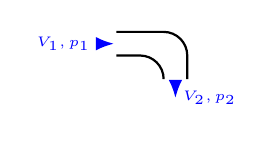
\begin{tikzpicture}[>=Latex,scale=0.3,baseline=(current bounding box.center)]
\draw[thick] (0,1) -- (2,1) arc (90:0:1) -- (3,-1);
\draw[thick] (0,0) -- (1,0) arc (90:0:1) -- (2,-1);
\draw[->, blue, thick] (-0.8,0.5) -- (-0.1,0.5) node[left=-1pt, pos=0]{\fontsize{3.5}{4.5}\selectfont $V_1, p_1$};
\draw[->, blue, thick] (2.5,-1.1) -- (2.5,-1.8) node[right=-1pt, pos=1]{\fontsize{3.5}{4.5}\selectfont $V_2, p_2$};
\end{tikzpicture}
\\
公式与计算链：
1. 算速度：$V_1 = \frac{4Q}{\pi D_1^2} = 1.415$ m/s, $V_2 = \frac{4Q}{\pi D_2^2} = 5.659$ m/s.
2. 算出口表压：由能量方程 $p_2 = p_1 - \frac{1}{2}\rho(V_2^2 - V_1^2) = 150000 - 500 \cdot (5.659^2 - 1.415^2) = 135.0$ kPa.
3. 取流体为控制体 (CV), 列分量动量方程 (设 $x$ 向流入, $y$ 向流出)：
   $x\text{向：}\quad p_1 A_1 - F_{gx} = \rho Q (0 - V_1) \Rightarrow F_{gx} = p_1 A_1 + \rho Q V_1$.
   代入：$A_1 = 0.0707$ m$^2$, $p_1 A_1 = 10605$ N, $\rho Q V_1 = 141.5$ N $\Rightarrow F_{gx} = 10.75$ kN.
   $y\text{向：}\quad 0 - p_2 A_2 + F_{gy} = \rho Q (V_2 - 0) \Rightarrow F_{gy} = p_2 A_2 + \rho Q V_2$.
   代入：$A_2 = 0.0177$ m$^2$, $p_2 A_2 = 2385$ N, $\rho Q V_2 = 566$ N $\Rightarrow F_{gy} = 2.95$ kN.
4. 流体对管作用力为管对流体受力 $F_{gx}, F_{gy}$ 的反力：
   $F_x = -F_{gx} = -10.75$ kN, $F_y = -F_{gy} = -2.95$ kN.

\subq{完整模板：串并联管网最小过程分}
串联：$Q$相同，$V_i$不同，$h_L=\sum(\lambda_iL_i/d_i+\sum\zeta_i)V_i^2/(2g)$。并联：上下游节点水头差相同，$h_{L,a}=h_{L,b}$，且$Q=Q_a+Q_b$。若题给粗糙度，湍流支路每条都要独立查$\lambda_i$。
\subq{完整模板：孔板/文丘里/皮托与流量计}
皮托：$V=C\sqrt{2\Delta p/\rho}$。文丘里/孔板：先把压差计换成$\Delta p$，再写
\fmlb{Q=C_dA_0\sqrt{\frac{2\Delta p}{\rho(1-\beta^4)}}\,,\quad \beta=d_0/d}
若题给水银压差计，常用$\Delta p=(\rho_{Hg}-\rho)g\Delta h$；若为空气管，管内气体密度可忽略。
\errq{母题1最后检查卡}
1 截面编号是否完整；2 大水面$V=0$是否使用；3 表压/绝压是否分清；4 每个局损速度是否取对；5 $Re$是否决定层/湍；6 泵/水轮机符号是否反；7 CV受力是否最后取反；8 单位是否从cm、h、kPa换到SI。
\idq{母题1考场定位卡：问什么写什么}
问$Q$：两自由液面列PVZ，未知只留$Q$，把$V_i=Q/A_i$代入损失项。问$p_A$：选最近已知压力截面到A点，不要跨全系统。问$h$或安装高度：先给最低允许压强，再反推高程。问$P$：先求扬程/水头$H$，再$P=\rho gQH$并乘/除效率。问$F$：先PVZ得$V,p$，再CV动量。
\formq{母题1答案骨架}
\fmlb{\begin{aligned}
&1.\ A_i=\pi d_i^2/4,\quad V_i=Q/A_i,\quad Re_i=V_id_i/\nu\\
&2.\ h_L=\sum \lambda_i(L_i/d_i)V_i^2/(2g)+\sum\zeta_iV_i^2/(2g)+\sum(V_1-V_2)^2/(2g)\\
&3.\ z_1+p_1/(\rho g)+V_1^2/(2g)+H_p
=z_2+p_2/(\rho g)+V_2^2/(2g)+H_T+h_L\\
&4.\ \sum F_x=\rho Q(V_{2x}-V_{1x}),\quad \sum F_y=\rho Q(V_{2y}-V_{1y})
\end{aligned}}
第4行用于弯管/喷嘴反力题，求管或支座受力时对流体受力取反。
\subq{压力线/能量线题：画HGL/EGL或判断哪里压强最低}
水力坡线HGL=$z+p/(\rho g)$；能量线EGL=HGL+$V^2/(2g)$。沿程损失使线连续下降；局部损失竖直跳降；泵处跳升；水轮机处跳降；管径变大速度头减小，HGL可上升但EGL仍因损失下降。汽蚀看HGL对应的绝压是否低于汽化压。
\subq{粗糙度反推/光滑管求流量}
光滑湍流可用Blasius：$\lambda=0.3164/Re^{1/4}$，代入$h_f=\lambda(L/d)V^2/(2g)$可直接解$V$。已知实际$Q$反推粗糙度：先由$Q$算$V,Re$，再由能量方程反算$\lambda$，最后用Colebrook或题给公式反解$\varepsilon/d$。
\subq{管路题必须写的假设}
不可压、定常、一维平均速度；管段内速度取截面平均；大水面速度忽略；局部损失系数按题给；动能修正系数未说明取$\alpha=1$；若题说短管，可忽略沿程；若题说长管，沿程不可忽略。
\errq{母题1高频扣分点}
把下游背压/出口内压混成一个；把泵扬程写成压力增量但单位没除$\rho g$；把水轮机输出功率写成泵输入功率；并联支路误设$Q$相等；串联变径误设$V$相等；压差计方向反；法兰受力未取反。
% ==================== SECTION 2 ====================
% ---- 母题1归位：静水/CV/管路/通用检查 ----
\iffalse
% 旧第二页散装缓冲区：此段把静水、CV、运动学、势流、可压、粘性、边界层、查表和通用检查混排在一起。
% 现在不作为可见正文输出；对应内容已按“母题/子题/信息库”归入第一页基础信息库及后续各母题。
% 后续若发现某个具体句子在对应母题下缺失，再从此段精确迁移。
\stepq{静力学、运动学、张量模型速解}
\errq{压强单位换算}
$1{\rm kPa}=10^3{\rm Pa}$；$1{\rm mmHg}=133.3{\rm Pa}$；水头$h=p/(\rho g)$。表压$p_g=p_{\rm abs}-p_a$；绝压进入汽蚀、气体状态方程；表压进入多数水力计算。
\stepq{平面闸门答题骨架}
1 取形心深度$h_C$。2 合力$F=\rho gh_CA$。3 压力中心：竖直平面$y_D=y_C+I_C/(y_CA)$；倾斜平面沿板长坐标同式，$h_C=y_C\sin\theta$。4 对铰点列力矩求拉力/反力。写明“压力分布为三角形或梯形”。
\stepq{曲面闸门答题骨架}
水平分量$F_x$等于曲面在竖直投影面上的静水压力；竖直分量$F_y$等于曲面上方压力体水重，方向看压力体在曲面哪侧。合力$F=\sqrt{F_x^2+F_y^2}$，作用线由力矩或过圆心性质定。
\conceptq{相对平衡}
容器水平加速度$a$：自由液面满足$dp=0$，$g\,dz+a\,dx=0$，故$\tan\alpha=a/g$。竖直加速向上$a$：等效重力$g+a$；向下$a$：$g-a$。旋转容器：$p/\rho+gz-\omega^2r^2/2=C$，自由面$z=\omega^2r^2/(2g)+C$。
\stepq{浮力和稳定}
浮力$F_B=\rho gV_{\rm disp}$，$V_{\rm disp}$为排开液体体积，作用于该体积形心。稳定判断：小倾角后浮心移动，重心$G$低于定倾中心$M$稳定；题若只问浮力，直接排水体积。
\formq{迹线/流线/脉线}
流线：固定时刻速度场切线，$dx/u=dy/v=dz/w$。迹线：单个质点轨迹，解$dx/dt=u(x,y,z,t)$。脉线：同一注入点不同时刻质点连线。定常流三者重合；非定常不能混写。
\stepq{加速度题模板}
$a_x=u_t+uu_x+vu_y+wu_z$，$a_y=v_t+uv_x+vv_y+wv_z$，$a_z=w_t+uw_x+vw_y+ww_z$。若只给二维定常，去掉$t,z$项。题问“当地/迁移”分别对应$\partial/\partial t$和对流项。
\stepq{应力张量标准解}
平面单位法向$\bm n=(n_x,n_y,n_z)^T$。应力矢量$\bm t=P\bm n$。法向应力$\sigma_n=\bm t\cdot\bm n$。切应力大小$\tau=\sqrt{|\bm t|^2-\sigma_n^2}$。夹角$\cos\alpha=\sigma_n/|\bm t|$。若问垂直平面分量，答案为$\sigma_n\bm n$。
\conceptq{应力对称原因}
无体偶力、微元角动量平衡给$p_{xy}=p_{yx}$，$p_{xz}=p_{zx}$，$p_{yz}=p_{zy}$。作用：张量独立分量从9个减到6个；做题时矩阵若不对称，通常题设有误或需取对称部分。
\conceptq{流体微团运动分解}
速度梯度$\nabla\bm V$可分解为平移、线变形率、角变形率、旋转。二维不可压时$u_x+v_y=0$；角速度$\omega_z=(v_x-u_y)/2$；角变形率$\varepsilon_{xy}=(u_y+v_x)/2$。
\quickq{维数分析常用组合}
阻力问题$F=f(\rho,\mu,V,L)$：$F/(\rho V^2L^2)=\Phi(Re)$。自由液面重力波常有$Fr=V/\sqrt{gL}$。表面张力小尺度常有$We=\rho V^2L/\sigma$。可压缩高速常有$Ma=V/a$。
\formq{伯努利、动量、能量方程模型速解}
\formq{伯努利适用性}
理想无粘：沿流线；无旋势流：全场任意点。实际管路：用机械能方程加$h_f,\sum h_\zeta,H_p,H_T$。非定常势流：$\partial\varphi/\partial t+V^2/2+p/\rho+gz=C(t)$。
\subq{弯管受力：已知Q/管径/进出口压强/转角，求支座反力}
对流体列动量，入口压力推入、出口压力推入控制体内部。若入口$x$向、出口转角$\alpha$：速度向量$\bm V_1=(V_1,0)$，$\bm V_2=(V_2\cos\alpha,V_2\sin\alpha)$。支座对流体力$\bm R$求出后，流体对管道力$-\bm R$。
\subq{射流冲板：已知射流V/Q与板运动，求冲击力/功率}
固定平板正撞：$F=\rho QV$。移动平板速度$u$：相对流量$\rho A(V-u)$，力$F=\rho A(V-u)^2$。功率$P=Fu$，最大功率常在$u=V/3$。斜板按法向动量变化。
\subq{喷嘴/水枪反力：已知入口压强/出口速度/流量，求握持力}
喷嘴出口表压近似0，入口压力加速流体：$p_1A_1-p_2A_2+R_x=\rho Q(V_2-V_1)$。若求握持力，取流体对喷嘴反力。先由伯努利或连续求$V_2,Q$。
\idq{通用题干关键词套写索引}
\formq{静水压/伯努利/动量}
先判断对象：静止液体$\to$静水压；沿流线能量$\to$Bernoulli/机械能；弯管喷嘴射流受力$\to$控制体动量。不要一个方程包打天下。
\formq{表值未算出时}
写“查表得$M=...,\lambda=...,\beta=...,\nu(Ma)=...$”，再把后续公式完整列出；未算表值也保留查表输入和回代链。
\stepq{标准卷面模板}
“本题属于\underline{\hspace{1cm}}模型。假设\underline{\hspace{1cm}}。控制方程为\underline{\hspace{1cm}}。由边界条件\underline{\hspace{1cm}}得未知量。代入数值得\underline{\hspace{1cm}}。物理判断：单位正确、方向正确、状态合理。”
\stepq{通用数值题公式链骨架}
\formq{应力张量指定平面}
已知应力张量$P$和单位法向$\bm n$：应力矢量$\bm t=P\bm n$；法向应力标量$t_n=\bm t\cdot\bm n$；法向分量$t_n\bm n$；切向分量$\bm t-\bm t_n\bm n$。夹角用$\cos\alpha=t_n/|\bm t|$。
\errq{高风险易混概念对照}
\symq{$p_0,p^*,p_e,p_b$}
$p_0$滞止压；$p^*$临界截面静压；$p_e$出口截面内静压；$p_b$背压/外界压。只有部分状态$p_e=p_b$。阻塞时收缩喷管$p_e=p^*$，不等于更低的$p_b$。
\symq{平均速度/最大速度/摩擦速度}
$\bar u$是截面平均；$u_{\max}$是中心最大；$u_\tau=\sqrt{\tau_w/\rho}$不是实际流速，而是由壁剪定义的速度尺度。壁律题用$u_\tau$。
\symq{表面积/迎风面积/截面积}
管流连续用截面积$\pi d^2/4$；平板摩擦用湿表面积$Lb$或$2Lb$；绕流阻力用迎风面积；静水压力用受压面积投影或实际面积，别混。
\errq{绝压/表压}
气体状态方程、汽化压、声速问题用绝压/绝温。水力能量方程两端同大气时可用表压。压力表读数通常是表压。
\idq{按题干关键词选公式}
\stepq{“定常一维绝热”}
若无摩擦激波，等熵；若有激波，分段等熵+激波关系；若有摩擦热交换，本表不套等熵，按题给关系。
\stepq{“平均时均速度”}
通常湍流统计量$\bar u$；若在管内，用壁律或平均速度公式，不是瞬时速度。雷诺应力$\overline{u'v'}$来自脉动相关。
\stepq{“完全发展”}
速度分布不随流向变，$\partial u/\partial x=0$，但压强仍沿流向下降。充分发展层流可解析；入口段不能直接用H--P。
\conceptq{“逆压梯度”}
$dp/dx>0$，流体沿流动方向压力升高，近壁减速，可能分离。顺压梯度$dp/dx<0$则加速，分离不易发生。
\formq{“压力中心/形心”}
形心用于算合力大小；压力中心用于合力作用点。压力中心在形心以下，除非面积水平或压强均匀。
\errq{计算细节防错}
\errq{单位统一}
面积：$1{\rm cm^2}=10^{-4}{\rm m^2}$；粗糙度mm转m；运动粘度$1{\rm mm^2/s}=10^{-6}{\rm m^2/s}$；温度用K；角度查表通常用度，计算三角函数确认模式。
\symq{截面积}
圆管$A=\pi d^2/4$，半径题$A=\pi R^2$。环形面积$A=\pi(R_o^2-R_i^2)$。平板流每单位宽度时$Q'=\int udy$，总流量$Q=bQ'$。
\symq{水头与压力}
$p/\rho g$单位是m。能量方程每一项都用m时，泵扬程$H_p$也是m；功率再乘$\rho gQ$。用压力形式时每项是Pa，损失为$\Delta p=\rho gh$。
\lookq{查表/异常回退}
查表写法：查\_\_表，输入\_\_，读得\_\_；需插值写“线性插值”。异常先按：单位、模型、边界、支路、符号回退。$M<0$或$p_{\rm abs}<0$查绝压/表压；$\dot m$不守恒回连续；$h_L<0$查泵/水轮机符号；$Re$判型冲突换层/湍公式；激波后$Ma_2>1$或$p_2<p_1$查表输入；泵入口$p_B<p_v$说明高度/损失过大。
\errq{方向检查}
力的方向若不确定，先假设正向，算出负值表示反向。动量方程一定是“外力合力=流出动量流率-流入动量流率”。
\errq{结果合理性}
收缩喷管未阻塞$Ma<1$；正激波后$Ma_2<1$；膨胀波后$M$增大、$p$降低；泵入口高度越大入口压越低；边界层厚度沿程增大。
\quickq{可直接写的结论句}
\formq{湍流句}
“湍流时速度可分解为时均量和脉动量，脉动相关产生雷诺应力，工程上常通过经验摩擦系数或壁律求解。”
\idq{题图识别+查表+公式链}
\idq{题图一眼选模型}
\par\noindent \renewcommand{\arraystretch}{1.15}\begin{tabular}{|p{0.22\linewidth}|p{0.70\linewidth}|}
\hline U管/压差计 & 同高同压链；$\Delta p=(\rho_m-\rho)g\Delta h$；振荡$T=2\pi\sqrt{L/2g}$\\ \hline
闸门/曲面 & 平面$F=\rho gh_CA,\;y_D=y_C+I_C/(y_CA)$；曲面$F_x=$投影，$F_y=$压力体\\ \hline
弯管/喷嘴 & 取管内流体CV：$\sum\bm F=\rho Q(\bm V_2-\bm V_1)$；题问管受力最后取反\\ \hline
射流冲板 & 固定正撞$F=\rho QV$；动板相对速度$V-u$；斜板按方向分量列动量\\ \hline
源+均流 & 驻点$r=Q/(2\pi U)$；分界流线常取$\psi=Q/2$；墙面先镜像\\ \hline
圆柱/环量 & $v_\theta=-2U\sin\theta+\Gamma/(2\pi a)$；$C_p=1-(v_\theta/U)^2$；$L'=\rho U\Gamma$\\ \hline
Laval/内激波 & 波前等熵$\to$正激波$\to$波后新$p_{02}$等熵；喉部不等于一定$Ma=1$\\ \hline
楔角/膨胀角 & 压缩角：斜激波，$Ma_{n1}=Ma_1\sin\beta$；凸角：PM，$\nu_2=\nu_1+\delta$\\ \hline
泵/水轮机 & 泵吸水看汽蚀绝压；水轮机$P=\eta\rho gQH_T$；局部损失用所在管段速度\\ \hline
边界层/两层流 & 平板用$Re_x,\bar C_f,\delta$；两层Couette速度连续、剪应力连续，$\tau=U/(h_1/\mu_1+h_2/\mu_2)$\\ \hline
\end{tabular}\par\noindent \renewcommand{\arraystretch}{1}
\formq{公式链：已知-中间量-目标量}
静水$h\to p\to F/M$；管路$Q,d\to V\to Re,\lambda,\zeta\to h_L$；CV$Q,A,p\to V,\dot m\to F$；势流$\phi/\psi\to V\to p$；可压/波$M,A/A^*,p_0,T_0,Ma_1,\theta\to$查表$\to p,T,\dot m,p_{02}$；边界层$Re\to\delta,C_f\to D$。
\stepq{按图像补充的模型第一步}
\subq{玻璃弯管放水：已知管形/初始水位/阀门，求压强分布和排空时间}
看见竖直段+倾斜段+阀门：未开阀时静水压分布$p=p_a+\rho g\Delta z$，只看竖直高度。开阀排空时间：沿流线伯努利求出口$V=\sqrt{2gH_{\rm eff}}$，再用液面下降连续方程积分。
\conceptq{雷诺输运定理题}
系统量变化=控制体内变化+穿过控制面的净流出。定常时控制体内变化为0。动量方程、质量守恒都是它的特例。
\idq{动力学/应力题干模型压缩}
\formq{应力张量+指定平面}
条件：给$P$和单位法向$\bm n$，目标为应力矢量、垂直分量、夹角。公式链：$\bm p_n=P\bm n$，$\bm p_N=(\bm p_n\cdot\bm n)\bm n$，$\bm p_T=\bm p_n-\bm p_N$，$\alpha=\cos^{-1}\frac{\bm p_n\cdot\bm n}{|\bm p_n|}$。
\formq{给应力分布求平面上一点}
先把点坐标代入$p_{xx},p_{xy},p_{yy}$得到矩阵$P$。平面$x+3y+z+1=0$法向$\bm n=(1,3,1)/\sqrt{11}$。同样$P\bm n$，再分解法向/切向。
\symq{由$\nabla\cdot P=-\rho\bm f$求体力}
散度按行求：$(\nabla\cdot P)_x=\partial p_{xx}/\partial x+\partial p_{xy}/\partial y+\partial p_{xz}/\partial z$，其余同理。最后$\bm f=-(\nabla\cdot P)/\rho$。
\stepq{正交曲线坐标散度}
若选做，核心是尺度因子$h_i$。圆柱坐标向量散度：$\nabla\cdot\bm A=\frac1r\frac{\partial(rA_r)}{\partial r}+\frac1r\frac{\partial A_\theta}{\partial\theta}+\frac{\partial A_z}{\partial z}$。张量散度需查教材公式，不要现场硬推。
\subq{弯玻璃管放水：已知竖直段/倾斜段/阀门，求静压和排空时间}
未开阀压力分布只由高度决定：从自由面向下$p=p_a+\rho gh$；倾斜段同样用竖直高度，不用管长。排空时间：液面高度$H(t)$，出口$V=\sqrt{2gH_{\rm eff}}$，$A_{\rm tank}dH/dt=-A_oV$积分。
\formq{速度场$u=3x^2-3y^2,v=-6xy$}
速度势：$\varphi=x^3-3xy^2+C$。流函数：$\psi=3x^2y-y^3+C$。速度势线$\varphi=C$，流线$\psi=C$。
\symq{$u=2cxy,v=c(a^2+x^2-y^2)$}
连续：$u_x+v_y=2cy-2cy=0$。旋度：$v_x-u_y=2cx-2cx=0$，无旋。$\varphi=\int2cxy\,dx=cx^2y+f(y)$，由$\varphi_y=cx^2+f'=c(a^2+x^2-y^2)$得$f=ca^2y-cy^3/3$。$\psi_y=u$求$\psi=cxy^2+g(x)$，再由$-\psi_x=v$定$g=-ca^2x-cx^3/3$。
\stepq{均匀流绕长钝体上坡}
无穷远均匀流$U$，已知A、B在同一流线。理想不可压无旋沿同一流线伯努利：$p_A+\rho gz_A+\frac12\rho V_A^2=p_B+\rho gz_B+\frac12\rho V_B^2$。若B点速度由势流叠加求，代入求高度或压差。
\stepq{风洞/多波相交题}
题面缺图时：超声速风洞内通常用喷管/试验段面积比求$M$，再用等熵关系求$p,T,\rho,V$。若有激波，按位置分段。答案必须先补完整题图或数据。
\formq{Re判层/湍}
水管$d=0.2,V=1,\nu=10^{-6}$：$Re=2\times10^5$，湍流。油管$d=0.15,V=0.2,\nu=2\times10^{-5}$：$Re=1500$，层流。圆管临界约2300。
\conceptq{“证明满足连续方程”}
直接算$\nabla\cdot\bm V$。若为二维：$u_x+v_y=0$。写“故不可压连续方程满足”。若不为0，说明该速度场不可能表示不可压流。
\idq{“判断有旋否”}
二维：$\Omega_z=v_x-u_y$。三维：$\nabla\times\bm V$。若为0，无旋，可求势函数；若非0，不能全场定义单值势函数。
\formq{“写流线方程”}
定常：$dy/dx=v/u$。分离变量积分。非定常问某时刻流线，先把$t=t_0$代入速度场再积分。
\formq{“写迹线方程”}
解ODE：$dx/dt=u(x,y,t)$，$dy/dt=v(x,y,t)$，带初始条件$x(t_0)=x_0,y(t_0)=y_0$。不要用$dy/dx=v/u$替代。
\stepq{“求流量”}
均匀速度$Q=VA$；非均匀$Q=\int_Au\,dA$。圆管轴对称$Q=2\pi\int_0^Ru(r)rdr$。平板单位宽$q=\int_0^hu(y)dy$。
\stepq{“求压强分布”}
静止流体$p=p_a+\rho gh$。势流定常$p=p_\infty+\frac12\rho(U_\infty^2-V^2)$。管路沿程压降由损失或H--P。可压缩等熵由$p_0/p(M)$。
\stepq{“求功率”}
泵/水轮机$P=\rho gQH$；阻力功率$P=DU$；剪切拖动功率$P=FU$；射流对动板功率$P=Fu$。注意效率。
\errq{“判断能不能用伯努利”}
同一流线、定常、不可压、无粘或损失可忽略。若有泵/损失，用机械能方程。若跨激波，不可用同一个伯努利常数。
\subq{闸门铰链：已知水深/闸门尺寸/铰点，求合力、压力中心、拉力}
题面有闸门、铰链、拉索：$F=\rho gh_CA$，$y_D=y_C+I_C/(y_CA)$，对铰链取矩：$T l_T=F l_F+G l_G$。若两侧有水，分别算两侧压力再相减。
\subq{曲面闸门/浮体：已知曲面几何和水深，求水平/竖直分力或浮力}
题面有圆弧闸门/半圆柱：水平分量=投影面压力；竖直分量=压力体重。若物体可浮起，加上浮力$\rho gV_{\rm disp}$和自重平衡。
\subq{U管相对平衡：已知容器加速度/旋转，求液面差或压差}
题面容器加速或旋转：先写等效体力，压强梯度$\nabla p=\rho(\bm g-\bm a)$。自由液面垂直于等效重力。U管两端压差再用液柱关系。
\formq{速度场+应力}
先算速度梯度，再牛顿粘性应力：$\tau_{xy}=\mu(u_y+v_x)$，正应力含压强$-p+2\mu u_x$。若只给应力张量，直接$P\bm n$。
\formq{伯努利+动量}
喷嘴/弯管常先用伯努利求$V,Q$，再用动量求力。不要只写一个方程；速度未知时动量方程不能闭合。
\conceptq{自由涡}
自由涡$v_\theta=C/r$，环量$\Gamma=2\pi r v_\theta=2\pi C$常数。压强径向平衡$dp/dr=\rho v_\theta^2/r$，液面凹陷。
\conceptq{强迫涡}
强迫涡$v_\theta=\omega r$，像刚体旋转。$dp/dr=\rho\omega^2r$，自由面$z=\omega^2r^2/(2g)+C$。
\varq{多出口分流}
连续：$Q_{\rm in}=\sum Q_{\rm out}$。动量方程每个出口都要加$\rho Q_i\bm V_i$。若速度大小相同但方向不同，向量不能当标量相加。
\conceptq{压力恢复/扩压器}
亚声速扩压速度降、压力升；若逆压梯度过大，边界层分离，实际压力恢复低。超声速扩压需先激波减速。
\symq{密度/压强/温度}
液体静压$p=p_a+\rho gh$。理想气体$p=\rho RT$。等温气体$\rho\propto p$。等熵气体$p/\rho^\gamma=C$，$T\rho^{1-\gamma}=C$。
\quickq{动量通量}
一维均匀截面动量流率$\rho Q\bm V$。非均匀需$\int_A\rho\bm V(\bm V\cdot\bm n)dA$，常引入动量修正系数。
\formq{雷诺数}
圆管$Re=Vd/\nu$；平板$Re_x=Ux/\nu$；小球$Re=Ud/\nu$。特征长度随问题变，不要固定用直径。
\idq{符号解释表：看到符号就知道干什么}
\symq{$\rho,\mu,\nu$}
$\rho$密度，$\mu$动力粘度，$\nu=\mu/\rho$运动粘度。Re题优先用$\nu$；剪应力题优先用$\mu$。单位：$\mu$为Pa·s，$\nu$为$m^2/s$。
\symq{$Q,\dot m,V,\bar u$}
$Q$体积流量，$\dot m=\rho Q$质量流量，$V$常为平均速度，$\bar u$明确表示截面平均/时均。圆管层流中心速度$u_{\max}=2\bar u$。
\symq{$p,p_g,p_0,p^*$}
$p$可能是绝压，$p_g$表压，$p_0$滞止压，$p^*$临界静压。气体状态方程必须绝压；水力方程可统一表压。
\symq{$h_f,h_\zeta,H_p,H_T$}
$h_f$沿程损失，$h_\zeta$局部损失，$H_p$泵扬程，$H_T$水轮机水头。能量方程中损失总在被消耗一侧。
\symq{$\delta,\delta^*,\theta$}
边界层名义厚度、位移厚度、动量厚度。$\delta$看速度达到$0.99U$，后两者由积分定义。
\symq{$u_\tau,y^+,u^+$}
摩擦速度$u_\tau=\sqrt{\tau_w/\rho}$；无量纲壁距$y^+=yu_\tau/\nu$；无量纲速度$u^+=u/u_\tau$。用于湍流近壁，不用于普通层流H--P。
\symq{$\nu(Ma)$}
Prandtl--Meyer函数，不是运动粘度$\nu$。膨胀波用$\nu(Ma)$，粘性Re用运动粘度$\nu$，看上下文。
\stepq{流程A：给速度场}
1 算散度。2 算旋度。3 若散度0求$\psi$；若旋度0求$\phi$；若问流线用$dy/dx=v/u$；若问加速度用当地+迁移。4 若给粘度求应力，再速度梯度。
\stepq{流程B：给静止液体图}
1 选自由液面为$p_a$。2 沿竖直高度算压强。3 平面用形心，曲面分水平/竖直。4 求铰链/拉力时对铰点取矩。
\stepq{流程C：给管路图}
1 标点1、2，通常选大水面/压力表/出口。2 算各管段$V,Re,\lambda$。3 写能量方程含$h_f,h_\zeta,H_p/H_T$。4 解压力、扬程或功率。
\errq{错2：把0.528到处用}
0.528是空气等熵$Ma=1$时$p^*/p_0$。只有截面临界才用。文丘里喉部若$Ma<1$不能用。
\errq{错4：面积比支路选错}
$A/A^*>1$有两个$M$。收缩管取亚声速；Laval扩张段根据背压和题意取亚/超声速。无激波设计通常取超声速。
\errq{错7：压力中心公式乱用}
$y_D=y_C+I_C/(y_CA)$中的$y$是沿平面从自由液面交线量的坐标；竖直深度要乘$\sin\theta$。
\errq{错8：动量方程标量化}
弯管、斜板必须用向量分量。速度大小不变不代表动量不变，方向变也有力。
\errq{错9：局部损失速度取错}
局部元件在哪个管段，就用哪个管段速度。突扩/突缩常需要前后速度，不要全用主干管速度。
\errq{错10：表压绝压混用}
压力表读数是表压；汽化压和气体方程用绝压。能量方程若两点同大气，可用表压统一。
\errq{错14：源涡原点直接用}
点源、点涡在奇点处模型失效，速度/压强发散。题通常只问奇点外区域。
\errq{错15：忘记单位换算}
cm$^2$、mm、kPa、mm$^2$/s最容易错。写表前先统一SI单位。
\stepq{标准解模板：静水压}
解：取自由液面为基准，形心深度$h_C=\cdots$。合力$F=\rho gh_CA=\cdots$。压力中心$y_D=y_C+I_C/(y_CA)=\cdots$。由力矩平衡$\sum M_O=0$得所求力$\cdots$。
\stepq{标准解模板：动量}
解：取包围弯管/喷嘴的控制体。连续方程得$Q=AV$。动量方程$\sum F_x=\rho Q(V_{2x}-V_{1x})$，$\sum F_y=\rho Q(V_{2y}-V_{1y})$。解得壁面对流体力，所求管受力为反向。
\stepq{标准解模板：管路}
解：选1、2截面列机械能方程。各段速度$V_i=Q/A_i$，$Re_i=V_id_i/\nu$，查得$\lambda_i$。总损失$\sum\lambda_iL_i/d_i\,V_i^2/(2g)+\sum\zeta_jV_j^2/(2g)$。代入得$H_p/H_T/p$。
\stepq{补充模型：自由面与涡}
\conceptq{自由涡液面}
$v_\theta=C/r$，径向平衡$dp/dr=\rho C^2/r^3$。自由面$p=p_a$且竖向静压，得$z=C_0-C^2/(2gr^2)$，中心凹陷。适用于排水旋涡外部近似。
\conceptq{强迫涡液面}
$v_\theta=\omega r$，$dp/dr=\rho\omega^2r$，自由面$z=\omega^2r^2/(2g)+C$，抛物面。容器旋转题用这个。
\conceptq{复合涡}
核心强迫涡、外部自由涡，交界处速度连续。常用于实际旋涡近似。压强分布分段积分。
\lookq{教材查找建议}
正激波表、斜激波表、PM表、面积--马赫表、Moody图、阻力系数图、常见截面惯性矩表、物性表。速查表里不要抄全表，只写“什么时候查、查完怎么用”。
\stepq{考试先后顺序}
先做能套模板的：静水压、速度场、管路、喷管、边界层。再做需查表的激波/PM。最后做推导证明题。未闭合题先写模型和控制方程拿步骤分。
\errq{数值题通用检查}
压力不能低于绝对零；水泵入口绝压不能随便小于汽化压；质量流量在同一管内守恒；激波后静压上升；膨胀后静压下降；边界层厚度不应超过特征长度太多。
\conceptq{概念题通用答法}
先定义，再说物理原因，再说公式或后果。例如问阻塞：定义$Ma=1$，原因信息不能上游传递，后果质量流量最大且不随背压增大。
\conceptq{证明题通用答法}
从守恒律或定义出发。连续方程来自质量守恒；Euler来自无粘动量；Bernoulli来自沿流线积分Euler；势流Laplace来自无旋+不可压；流函数Poisson来自涡量定义。
\idq{图像题通用答法}
先在图上标1、2截面、坐标方向、速度方向、压力方向、已知高度。图像题扣分多来自方向和截面选错。
\stepq{答题纸三行骨架}
1 “取控制体/流线/截面如图。” 2 “由连续/动量/能量/状态方程得...” 3 “代入题给数据，取正方向，故结果为...” 这三行至少保住结构分。
\quickq{高频小问速答}
\conceptq{为什么应力张量对称}
对微元取角动量矩平衡，若无体偶力，剪应力互等，故应力张量对称。用途：减少未知量，保证任意切面的应力由$P\bm n$唯一确定。
\conceptq{为什么Laplace}
不可压$\nabla\cdot\bm V=0$，又$\bm V=\nabla\phi$，所以$\nabla^2\phi=0$。无旋二维流函数同理$\nabla^2\psi=0$。
\conceptq{为什么Bernoulli沿流线}
无粘Euler方程沿流线积分，定常不可压时动能、压能、位能总和守恒。若无旋，常数可扩展到全场。
\conceptq{为什么粗糙度层流不用}
层流摩阻来自粘性剪切解析解，$\lambda=64/Re$；粗糙凸起若未破坏层流，公式中不出现粗糙度。湍流中粗糙度影响近壁结构。
\conceptq{为什么平板局部/平均系数不同}
局部$c_f(x)$随$x$变化；总阻力是沿全板积分的平均效果，所以用$\bar C_f$。尾部局部值不能代表总板阻力。
\conceptq{为什么管路损失用速度头}
损失本质是机械能耗散，工程上以单位重量能量表示。局部扰动强度通常与动压$\rho V^2/2$成正比，所以写成$\zeta V^2/(2g)$。
\conceptq{为什么压力中心低于形心}
静水压随深度线性增大，较深部分受力更大，合力作用点向深处偏移，故压力中心低于形心。
\conceptq{为什么动量方程要控制体}
流体不断进出，质点系统不好追踪。控制体形式用流入流出动量通量表达，适合弯管、喷嘴、射流等定常问题。
\conceptq{为什么流量要积分}
截面速度若不均匀，$VA$只适用于平均速度。真实流量是每个面积元的法向速度贡献积分：$Q=\int_A v_n dA$。
\errq{为什么表压可为负}
表压相对大气压定义，低于大气压时为负；绝压不能为负。汽蚀判断看绝压是否低于汽化压。
\conceptq{为什么泵入口最危险}
泵吸入侧压力最低，若安装高度大或损失大，入口绝压可能低于汽化压，先发生汽蚀。
\conceptq{为什么水轮机要扣损失}
上游总水头不是全部转化为轴功，一部分作为沿程/局部损失和下游剩余动能，剩余才是水轮机可利用水头。
\conceptq{为什么答案要写假设}
流体题公式都有适用条件。写“定常、不可压、无粘/充分发展/等熵”等假设，可以明确选用方程并获得过程分。
\quickq{常用平方/根号}
$\sqrt{2gH}\approx4.43\sqrt{H}$ m/s。$V^2/(2g)$：$V=1,2,5,10$ m/s时约$0.051,0.204,1.27,5.10$m。
\quickq{常用水柱压强}
$1$m水柱约$9.81$kPa；$10$m约$98.1$kPa；$10.33$m约1atm。水银$1$mm约133Pa。
\quickq{常用圆管面积}
$d=0.1$m，$A=7.85\times10^{-3}$；$d=0.2$m，$A=3.14\times10^{-2}$；$d=0.3$m，$A=7.07\times10^{-2}$。
\quickq{空气等熵速算}
$M=0.5$：$T_0/T=1.05,p_0/p\approx1.19$。$Ma=1$：$1.2,1.893$。$M=2$：$1.8,7.82$。$M=3$：$2.8,36.7$。
\quickq{层流圆管速算}
$Re=VD/\nu$。水$\nu\approx10^{-6}$，所以$V=1,d=0.1$时$Re=10^5$湍流；油$\nu=10^{-5}$时同条件$Re=10^4$。
\quickq{动量力速算}
水流$Q=0.01$m$^3$/s，$V=10$m/s，动量力$\rho QV=100$N。速度方向转90度，两个方向分量都要算。
\quickq{泵功率速算}
$P=\rho gQH$。水中$Q=0.01,H=10$m，水功率约981W。考虑效率0.7，轴功率约1.4kW。
\quickq{粗糙度速算}
$\varepsilon=0.2$mm，$d=0.2$m，则$\varepsilon/d=0.001$。题中“粗糙度$h$”通常就是$\varepsilon$。
\errq{管路答案数量级}
损失水头不应为负；泵扬程若小于总损失无法供水；水轮机可利用水头不能超过上下游总水头差。
\quickq{压力中心数量级}
矩形竖直板上边在自由面、高$h$，压力中心深度$2h/3$。若算到$h/2$上方，说明公式或坐标错。
\quickq{局部损失数量级}
$\zeta=1,V=2$m/s时损失约$0.204$m水头；$V=10$m/s时约$5.1$m。高速下局部损失很大。
\stepq{题目读数顺序}
先圈单位，再圈“忽略/不可忽略”，再圈“等熵/有激波/有损失”，最后圈要求量。很多错误来自漏掉“入口速度可忽略”或“表压”。
\errq{交卷前记忆卡}
静水压看高度；动量看方向；管路看损失；势流看叠加；喷管看$M$和背压；激波看分段；边界层看$Re$；粘性解析看边界条件。
\stepq{模板：速度场流程}
给$\bm V=(u,v,w)$。先写$\nabla\cdot\bm V=u_x+v_y+w_z=\cdots$，故是否不可压。再写$\nabla\times\bm V=(w_y-v_z,u_z-w_x,v_x-u_y)=\cdots$，故是否有旋。若无旋，$\phi=\int u dx+f(y,z)$，逐项定函数。
\stepq{模板：流线流程}
由流线微分方程$\frac{dx}{u}=\frac{dy}{v}$，代入$t=t_0$若非定常。整理为$M(x,y)dx+N(x,y)dy=0$，积分得$F(x,y)=C$。若与$\psi=C$一致，说明计算正确。
\stepq{模板：迹线流程}
由$\dot x=u(x,y,t),\dot y=v(x,y,t)$。先解$x(t)$，再代入解$y(t)$；带入初始条件确定常数。最后消去$t$或写参数方程。
\stepq{模板：应力流程}
单位法向先归一化。$\bm t=P\bm n$写成列向量。$\sigma_n=\bm n^T P\bm n$。$\tau=\sqrt{\bm t^T\bm t-\sigma_n^2}$。若题要分量，写$\bm t_N=\sigma_n\bm n,\bm t_T=\bm t-\bm t_N$。
\stepq{模板：闸门流程}
设水深方向坐标$y$，形心$y_C$，面积$A$，惯性矩$I_C$。$F=\rho g y_C\sin\theta A$。压力中心$y_D=y_C+I_C/(y_CA)$。对铰点取矩求未知力，注意力臂是几何垂距。
\stepq{模板：曲面流程}
投影面积$A_x$形心深$h_C$，$F_x=\rho gh_CA_x$。压力体体积$V_p$，$F_y=\rho gV_p$，方向由水压推曲面方向定。合力大小和方向$\tan\alpha=F_y/F_x$。
\stepq{模板：泵流程}
从吸水池水面到泵入口：求安装高度/汽蚀。从泵入口到出口或两水池：求泵扬程。不要把两个方程混成一个。汽蚀题必须用绝压。
\stepq{模板：水轮机流程}
选上游高水面和下游压力表/水面。机械能方程右侧加$H_T$，即流体失去的水头。$H_T$求出后$P=\eta\rho gQH_T$。
\stepq{压强题骨架}
写“压强随竖直深度线性变化，与容器形状无关”。再画压力分布三角形/梯形；力矩未算完也保留合力和作用点。
\stepq{速度场题骨架}
写散度、旋度两个算式。多数题至少一半分在这里。若能积分出$\phi$或$\psi$，再补。
\stepq{管路题骨架}
写完整机械能方程；若$\lambda$未查出，先保留$\lambda$符号。把$h_f,\sum h_\zeta,H_p,H_T$位置放对。
\conceptq{概念题骨架}
定义+原因+后果三段式。例：阻塞=喉部$Ma=1$；原因=扰动不能上传；后果=质量流量最大。
\conceptq{证明题骨架}
从定义写起：连续来自质量守恒，伯努利来自Euler沿流线积分，Laplace来自无旋不可压，流函数Poisson来自涡量定义。
\stepq{单位题骨架}
所有数值先写SI单位转换。老师看见单位转换，至少知道你没瞎代。
\stepq{静水矩形窗}
$F=\rho g(h_0+h/2)bh$；压力中心距窗顶$y=(h_0+h/2)+I_C/[(h_0+h/2)A]$，再换成题目坐标。
\stepq{静水圆形舱门}
$A=\pi R^2,I_C=\pi R^4/4$。$F=\rho gh_CA$，$y_D=y_C+R^2/(4y_C)$。
\stepq{浮力/吃水}
平衡$\rho_w gV_{\rm disp}=G$。若圆柱竖放，$V_{\rm disp}=Ah$；若横放，查/算圆缺面积。
\stepq{非恒定小孔出流}
$A_t dH/dt=-C_dA_o\sqrt{2gH}$，积分$t=\frac{2A_t}{C_dA_o\sqrt{2g}}(\sqrt{H_1}-\sqrt{H_2})$。
\stepq{皮托/静压管测速}
$p_0-p=\frac12\rho V^2$。若接U管，$p_0-p=(\rho_m-\rho)g\Delta h$。
\stepq{喷嘴反力}
$F_{\rm hold}\approx\rho QV+(p_e-p_a)A_e$，若出口对大气$p_e=p_a$，只剩动量项。
\subq{喷嘴法兰：已知$p_1$,$p_2$,Q,A，求法兰/螺栓受力}
取喷嘴内流体为控制体：$p_1A_1-p_2A_2+R_x=\rho Q(V_2-V_1)$。法兰螺栓受力为流体对喷嘴的反力，方向与$R_x$相反；出口对大气用表压$p_2=0$。
\varq{局部突扩}
$h=(V_1-V_2)^2/(2g)$。压力可能升高但总能量下降。
\quickq{泵效率/轴功率}
$\eta=\rho gQH/P_{\rm shaft}$。若求轴功率，$P_{\rm shaft}=\rho gQH/\eta$。
\quickq{水轮机效率/输出}
$P_{\rm out}=\eta\rho gQH_T$。若给输出功率反求$H_T=P/(\eta\rho gQ)$。
\subq{自由涡压差：已知环量/半径，求两点压差或液面凹陷}
$dp/dr=\rho C^2/r^3$，积分$p_2-p_1=\frac12\rho C^2(1/r_1^2-1/r_2^2)$。
\subq{强迫涡压差：已知角速度/半径，求压差或自由面高度差}
$dp/dr=\rho\omega^2r$，积分$p_2-p_1=\frac12\rho\omega^2(r_2^2-r_1^2)$。
\subq{气球受风：已知浮力/风速/阻力系数，求绳偏角}
净浮力$B=(\rho_a-\rho_g)gV-G$，风阻$D=C_D(0.5\rho_aU^2)A$。若细线与竖直夹角$\theta$，平衡得$\tan\theta=D/B$。
\errq{答案末尾检查}
每个答案后写单位；每个力题说明方向；每个压缩流题说明是等熵还是激波；每个粘性题说明层流还是湍流。
\lookq{Moody查图子链}
先判层流/湍流。湍流才用$Re$和$\varepsilon/d$查图。若题给“完全粗糙”，$\lambda$几乎与$Re$无关。
\lookq{物性表查表子链}
水温给出时查$\rho,\mu,\nu,p_v$。汽蚀题必须查$p_v$。空气题通常给$R,\gamma$，若不给取空气标准值。
\lookq{惯性矩查表子链}
压力中心题需要面积二次矩$I_C$，不是质量转动惯量。矩形$bh^3/12$，圆$\pi R^4/4$，三角形查表。
\stepq{三角函数角度}
激波/PM表多为度；计算器确认DEG。LaTeX/推导里弧度不影响公式，但数值代入会错。
\idq{题目图像再识别}
\miniimg{0.98}{assets/original_problem_schematics_generic.png}
\idq{图像：有大水面+管道+泵}
一定是机械能方程。大水面速度0、表压0。泵前若问安装高度，就是汽蚀；泵后若问压力/功率，就是扬程。
\quickq{图像：管道变径}
连续先给$V_1,V_2$。突扩有局部损失$(V_1-V_2)^2/(2g)$；渐扩看是否给扩压器效率或损失系数。
\quickq{图像：管道弯头}
局部损失$\zeta V^2/(2g)$用于能量；弯管受力用动量。两个问题不要混。
\idq{图像：喷口射流}
自由射流出口压力等于大气。速度由伯努利；反力由动量。射流打板再按板方向分解动量。
\idq{图像：两平板夹流体}
上板动下板静是Couette；有压差是Poiseuille；两者同时存在则叠加。两层流体加交界条件。
\quickq{图像：同心圆管/环隙}
若内外圆柱相对运动，是环隙Couette，速度分布可能含$\ln r$。若压差驱动，是环隙Poiseuille，查教材公式或由圆柱坐标积分。
\quickq{图像：旋转容器}
自由面抛物线。若问压强，$p/\rho+gz-\omega^2r^2/2=C$。若问液面高度差，$\Delta z=\omega^2(R_2^2-R_1^2)/(2g)$。
\quickq{图像：自由涡水面}
液面中心凹陷，$v_\theta=C/r$。与强迫涡相反：强迫涡中心低但外缘高为抛物面，自由涡近中心理论发散。
\quickq{图像：U形管振荡}
两个自由面高度差产生回复力，周期$2\pi\sqrt{L/(2g)}$。若管截面不等，需要用体积连续换算位移。
\idq{第一眼先判“物质模型”}
静止$\to$静水；无粘不可压$\to$Euler/Bernoulli/势流；可压无粘$\to$等熵/激波/膨胀；不可压有粘$\to$N--S/H--P/Couette/管损/边界层。
\idq{题目问“求什么”}
按输出量反推第一行：$p/H\to$静水压或能量；$Q/V\to$连续+压差/能量/阻塞；$F/R\to p,V,Q$后列CV动量；$\dot m,A,M\to$状态方程+等熵/面积--Ma；$D/\delta\to Re$判型后接$C_f/C_D$或边界层公式；$t\to$瞬时体积守恒微分方程；证明/说明/判断$\to$假设+主方程+边界+判据+结论。
\idq{题干给速度场$u,v,w$}
先算$\nabla\cdot V$和$\nabla\times V$；问轨迹写ODE，问流线写$dx/u=dy/v=dz/w$；问应力用速度梯度，问势/流函数用积分互求。
\idq{题干给容器、液面、压差计、闸门}
优先静水压链。自由液面$p=p_a$，同高同液等压；闸门先$F=\rho gh_CA$和压力中心，再对铰链取矩。
\idq{题干给管路、泵、阀、弯头、粗糙度}
先连续求$V$，再$Re$判层/湍，取$\lambda$或查Moody；机械能方程汇总$h_f+\sum h_\zeta$。汽蚀用泵入口绝压约束。
\idq{题干给喷嘴、射流、弯管受力}
能量求速度/压强，控制体动量求力：$\sum F=\sum_{\rm out}\rho QV-\sum_{\rm in}\rho QV$。题问管壁/法兰时取反。
\stepq{运动学长题}
流线：固定时刻速度场切线；迹线：单个质点轨迹；脉线/串线：同一点连续染色质点的位置集合；流体线/物质线：同一时刻相邻质点连线。定常时三线重合。计算：流线$\frac{dx}{u}=\frac{dy}{v}=\frac{dz}{w}$；迹线$\dot x=u(x,y,z,t)$带初值。加速度$D\bm V/Dt=\partial_t\bm V+(\bm V\cdot\nabla)\bm V$。
\conceptq{概念长答加分}
三句结构：定义+适用条件+后果/公式。例：边界层=高Re近壁薄层，条件是粘性只在壁附近重要，后果是外流可近似无粘、壁面满足无滑移并产生摩擦阻力和分离。
\idq{带教材查表/模型定位：补过程分}
\stepq{查教材表三行格式}
卷面四项：查\underline{\hspace{0.35cm}}表/图；输入\underline{\hspace{0.45cm}}；读得\underline{\hspace{0.45cm}}；代入\underline{\hspace{0.5cm}}；检查单位/支路/绝压表压。
\idq{模型冲突先判}
给$\mu,\nu,\varepsilon,C_D$优先粘性/阻力；给$\phi,\psi,\Gamma$优先势流；给$M,p_0,T_0,p_b$优先可压；给泵/阀/长管优先机械能；给“证明/说明”优先假设+方程+边界+结论。
\idq{题干图像/文字不全时}
不要空题：缺几何量/表值就设$x$或写“查表得…”。先写模型、主方程、查表输入$\to$输出$\to$回代链；固定编号索引不可靠，关键词和已知量判断更可靠。
\stepq{平板层流/矩形板摩擦型}
给$\mu,\rho,U,L,b$：$\nu=\mu/\rho,Re_L=UL/\nu$；层流$\delta=5L/\sqrt{Re_L}$，$D=\bar C_f(0.5\rho U^2)A,\bar C_f=1.328/\sqrt{Re_L}$。有转捩：$x_{cr}=Re_{cr}\nu/U$，分层流段+湍流段摩擦，$P=DU$。
\stepq{复杂题考场流程}
图表题：先写查表输入量和主公式，数值从教材补；长推导：假设$\to$控制方程$\to$边界条件$\to$结论；相似律冷门题：列变量，$\pi=X\rho^aV^bL^c$，说明主导准则。
\symq{模板：先写符号后代数}
不要边想边代。先写$Re=Vd/\nu=\cdots$，再写数值。公式正确即使数值错也能保分。
\stepq{模板：面积换算}
$A=\pi d^2/4=\pi(0.1)^2/4=7.85\times10^{-3}{\rm m^2}$。这类中间值可写在草稿区。
\stepq{模板：速度换算}
$V=Q/A$。若$Q$给$m^3/h$，先除3600。若给L/s，乘$10^{-3}$。
\stepq{模板：压强水头}
$p/(\rho g)=70000/(1000\times9.81)=7.14$m。kPa转水头直接除9.81。
\stepq{模板：雷诺数}
$Re=Vd/\nu$。把$\nu$写成科学计数法，防止$10^{-6}$漏掉。
\stepq{模板：损失水头}
$h_f=\lambda(L/d)V^2/(2g)$。先算$L/d$和速度头，再乘$\lambda$。
\stepq{模板：功率}
$P=\rho gQH$，水中可速算$P({\rm kW})\approx9.81QH$，$Q$用$m^3/s$。
\stepq{模板：风管/风扇}
气体也用压强水头$H=\Delta p/(\rho g)$。风扇需提供$H=\sum(\lambda L/d+\zeta)V^2/(2g)+$高度/速度项；轴功率$P=\Delta p\,Q/\eta=\rho gQH/\eta$。
\errq{模板：真空度/负表压}
表压$p_g=p_{\rm abs}-p_a$；真空度$p_v=p_a-p_{\rm abs}=-p_g$。U管同一静止连通液体同高压强相等，跨液柱加减$\rho gh$。
\stepq{模板：压力中心}
矩形竖直上边距液面$h_0$：$y_C=h_0+h/2$，$I_C=bh^3/12$，$y_D=y_C+I_C/(y_CA)$。
\conceptq{长推导/概念证明保分骨架}
\idq{证明题关键词卡}
固定结构：条件$\to$方程$\to$边界/积分路径$\to$化简$\to$结论限制。RTT/控制体：系统导数=CV局部项+CS通量项。Kelvin：$D\Gamma/Dt=\oint D\bm V/Dt\cdot d\bm l=0$。Lagrange：$\Gamma_0=0\Rightarrow\Gamma=0\Rightarrow\Omega=0$。Helmholtz：Kelvin+Stokes得涡线随体、涡管强度守恒。势函数单值：两路径差$=\oint\bm V\cdot d\bm l=\iint\Omega_n dA$。边界层积分：N--S沿$y$积分$\to\delta^*,\theta\to$Karman。非定常Bernoulli：Euler写成$\partial_t\bm V+\nabla(V^2/2)-\bm V\times\bm\Omega=-\nabla(p/\rho+\Pi)$；无旋得$\partial_t\phi+V^2/2+p/\rho+\Pi=f(t)$。
\formq{速度势与单值性}
无旋$\nabla\times\bm V=0$，单连通域内可令$\bm V=\nabla\phi$。证明路径无关：$\phi_P-\phi_0=\int_0^P\bm V\cdot d\bm r$；两路径差$=\oint\bm V\cdot d\bm l=\iint(\nabla\times\bm V)\cdot\bm n\,dA$，单连通且无旋$\Rightarrow0$。多连通域有点涡/环量时，速度可单值而$\phi$多值。不可压再给$\nabla^2\phi=0$。
\conceptq{Kelvin定理推出Lagrange定理}
理想无粘、正压$\rho=\rho(p)$、保守体力下，随体闭合线环量$\Gamma=\oint\bm V\cdot d\bm l$守恒。Lagrange定理：若某时刻处处无旋，则以后始终无旋；证法：任意小闭合线$\Gamma_0=0$，以后仍$\Gamma=0$；由Stokes，$\Gamma=\iint(\nabla\times\bm V)\cdot\bm n\,dA$，任意小面为0，故$\nabla\times\bm V=0$。物理句：无粘切应力不能自生/消灭微团旋转。
\quickq{涡线、涡管、涡通量}
涡线切向为涡量$\bm\Omega=\nabla\times\bm V$，方程$dx/\Omega_x=dy/\Omega_y=dz/\Omega_z$。涡通量$J=\iint_A\bm\Omega\cdot\bm n\,dA$；由Stokes，$J=\oint_{\partial A}\bm V\cdot d\bm l=\Gamma$。涡管侧面$\bm\Omega\cdot\bm n=0$，所以任意截面涡通量相等；微元涡管常写$\Omega_1A_1=\Omega_2A_2$。
\conceptq{Helmholtz涡定理答句}
理想、正压、保守体力：涡线随流体运动；涡管强度守恒；涡线不能在流体内部开始或终止，只能闭合、伸到边界或无穷远。考试只需写条件+三条结论。
\formq{涡量矩/随体守恒题}
二维不可压理想流：$D\Omega/Dt=0$，且随体面积$dA$不变，故$\Omega\,dA$随体守恒。若题问涡量矩，先写$\Gamma=\int\Omega dA$守恒，$x_c=\int x\Omega dA/\Gamma,\ y_c=\int y\Omega dA/\Gamma$；二阶矩$I=\int[(x-x_c)^2+(y-y_c)^2]\Omega dA/\Gamma$，用随体导数和一阶矩相消证明。
\errq{坐标、单位、负号}
压力式Pa：$p+\frac12\rho V^2+\rho gz$；水头式m：$p/\rho g+V^2/2g+z$。管路$z$向上为正，静水压深度$h$向下为正。压降$\Delta p=p_1-p_2>0$；沿程梯度常为$dp/dx<0$，H--P写$-dp/dx>0$。
\idq{题图决策卡}
\idq{图里有“自由液面”}
自由液面通常$p=p_a$；若水箱很大取$V\approx0$。若液面随时间动，必须接连续方程$A\,dh/dt=\pm Q$，不是只列伯努利。
\idq{图里有“压力表”}
表压进入能量方程可直接当$p/\rho g$；若题问汽蚀/蒸汽压，必须换绝压：$p_{\rm abs}=p_g+p_a$。
\idq{图里有“U形压差计”}
先写两连接点压力差。若测同一流体管路，常用$\Delta p=(\rho_m-\rho)g\Delta h$；若一端接大气，用$p-p_a=\rho_m g\Delta h$。
\idq{图里有“铰链+拉杆”}
别先求反力。先求水压力合力和压力中心，再对铰链取矩求拉力；最后若题要铰链反力，再用力平衡。
\idq{图里有“弯头/喷嘴出口”}
出口若射入大气，出口静压为大气压。支座力方向容易反：先求外界对流体力，再取相反即流体对管壁力。
\idq{图里有“泵在吸水侧”}
最高安装高度由泵入口最低允许绝压控制，不由泵功率直接控制。能量方程从水面列到泵入口。
\idq{图里有“水轮机”}
水轮机不是加能，是取能。能量式中$H_T$放在下游侧或从上游总水头中减去；功率$P=\eta\rho gQH_T$。
\idq{图里有“突然扩大/缩小”}
突扩损失常用$h=(V_1-V_2)^2/(2g)$；突缩或阀门按题给$\zeta V^2/(2g)$。速度取对应局部元件处速度。
\idq{图里有“平板零攻角”}
摩擦阻力用湿表面积，单面$Lb$，双面$2Lb$。空气和水同速同板，阻力差主要来自$\rho,\nu$导致的$Re$和$C_f$。
\symq{平均速度}
管路能量题用截面平均速度$V=Q/A$；边界层/壁律题里的$u(y)$是局部速度。
\errq{表压零点}
开口水面表压为0，不是绝压为0；涉及汽化压、气体状态方程时必须用绝压。
\errq{方向符号}
静水深度$h$常向下为正，能量方程高度$z$向上为正。CV截面压力永远推入，求管道/螺栓受力最后取反。
\symq{摩擦面积}
平板阻力题问单面/双面要看图；管内沿程损失不用外表面积，用$L/d$和速度头。
\quickq{局部损失速度}
不同管径时，每个阀门/弯头的$\zeta V^2/2g$用该元件所在管段速度。
\formq{应力题}
求某平面应力矢量直接$P\bm n$；法向分量是投影$(P\bm n)\cdot\bm n$，不是矩阵对角元。
\stepq{简答题首句索引}
先按题干原词写首句：N--S=牛顿流体动量方程；$Ma=V/a$=惯性/弹性量级，$Ma\le0.3$常忽略压缩；深水波=底床影响可忽略；水击波速=液体可压缩性+管壁弹性决定；渐变流=流线近似平行、同断面测压管水头近似常数；圆管层流剖面=抛物线，湍流剖面=丰满且有脉动；完全相似=主控$\pi$数全等，部分相似=只保主导准则。然后补：定义+机理+公式/限制。
\formq{连续介质}
连续介质假设：宏观尺度远大于平均自由程，把$\rho,p,\bm V$看成连续函数$F(x,y,z,t)$，才能用微积分写连续、动量、能量方程。
\conceptq{欧拉/拉格朗日}
欧拉法盯固定空间点，给$\bm V(x,y,z,t)$；拉格朗日法盯同一流体质点，给$\bm x(a,b,c,t)$。定常流中流线、迹线、脉线重合。
\formq{控制体/系统/质量动量能量守恒}
系统是固定流体质点集合，随流体运动；控制体是选定空间区域，流体可进出。雷诺输运：$\frac d{dt}\int_{\rm sys}b\,dm=\partial_t\int_{CV}\rho b\,d\forall+\int_{CS}\rho b(\bm V\cdot\bm n)dA$，取$b=1,\bm V,e,\bm r\times\bm V$即质量/动量/能量/动量矩。
外力=质量力+表面力+支反力，常见为重力、压力、剪切、支座/螺栓反力。力矩题用$\sum \bm M_O=\sum_{\rm out}\rho Q(\bm r\times\bm V)-\sum_{\rm in}\rho Q(\bm r\times\bm V)$；压力力$\bm F_p=\int p(-\bm n)dA$，均匀大气压闭面相消可用表压；旋转机械功率$P=M\omega$。
\conceptq{当地/迁移/随体导数}
$D\rho/Dt=\partial\rho/\partial t+u\rho_x+v\rho_y+w\rho_z$。当地：同一点随时间变；迁移：质点走到不同位置导致变。纳维-斯托克斯(N--S)：$\partial_t\bm V+(\bm V\cdot\nabla)\bm V=-\nabla p/\rho+\nu\nabla^2\bm V+\bm f$。答项意：左边=单位质量加速度(当地+迁移)，右边=压强力+粘性扩散力+质量力。
\conceptq{层流/湍流/渐变流}
圆管断面速度分布：层流分层有序、脉动小，$Re<2300$，$u=2\bar u(1-r^2/R^2)$为抛物线；湍流=时均+脉动，剖面更丰满，近壁$u^+=2.5\ln y^++5.5$或$1/7$次幂。Boussinesq涡黏把$-\rho\overline{u'_iu'_j}$类比为$\mu_t$乘时均速度梯度，$\mu_t$不是物性。渐变流：流线近似平行，同断面测压管水头$p/(\rho g)+z\approx C$。
\stepq{孔板/自由射流}
孔板节流：流通面积缩小，速度升高、静压降低，同时有局部损失，实际流量需乘流量系数。自由射流：出口后$p\approx p_a$，用横截面动量通量$\int\rho u^2dA$守恒/近似守恒，卷吸使射流宽度增大、中心速度衰减。
\quickq{常见速度剖面结果/1/n指数律}
\par\noindent \begin{tabular}{|p{0.42\linewidth}|p{0.52\linewidth}|}\hline
$u/U=\eta$ & $\delta^*=\delta/2,\ \theta=\delta/6,\ H=3$\\\hline
$u/U=\frac32\eta-\frac12\eta^3$ & $\delta^*=3\delta/8,\ \theta=39\delta/280,\ H=35/13$\\\hline
$u/U=\eta^{1/n}$；1/6律取$n=6$ & $\delta^*=\delta/(n+1),\ \theta=n\delta/[(n+1)(n+2)]$\\\hline
$u/U=\sin(\pi\eta/2)$ & $\delta^*/\theta\approx2.66,\ C_D\approx1.31/\sqrt{Re_L}$\\\hline
\end{tabular}
\formq{边界条件翻译表}
固壁：不穿透$\bm V\cdot\bm n=0$，有粘再加无滑移$\bm V=\bm V_w$。对称轴/管心：速度有限且$du/dr=0$。自由面：$p=p_a$，随时间动则接$A\,dh/dt=\pm Q$。两流体界面：速度连续、剪应力连续$\mu_1u_1'=\mu_2u_2'$。充分发展：$\partial u/\partial x=0,\ v=0$。远场：$V\to U_\infty$。
\lookq{高频计算/查表/控制体收口}
{\fontsize{4.35}{4.45}\selectfont
\textbf{目标量首行}：求$p$判静水/Bernoulli/等熵/激波；求$F$用CV或$p\,dA$或$C_DqA$；求$Q/\dot m$用连续、$\lambda$/H--P或可压$Ma$；求$Ma$用压比/面积比/波表；求$D$判$C_f$湿面积或$C_D$迎风面积；求$t$写$A\,dh/dt=\pm Q$。 
\textbf{泵/水轮机}：吸水$p_a/\rho g+z_0=p_B/\rho g+z_B+V^2/2g+h_L$，$p_B\ge p_v+\Delta p_{\rm safe}$，$NPSH_a=(p_B-p_v)/\rho g+V_B^2/2g$；水轮机$H_T=H_{\rm up}-H_{\rm down}-h_L,\ P=\eta\rho gQH_T$。 
\textbf{孔板/文丘里}：$\beta=d_0/d$，理想$Q=A_0\sqrt{2\Delta p/[\rho(1-\beta^4)]}$；实际$Q=C A_0\sqrt{2\Delta p/[\rho(1-\beta^4)]}$，$C$由$\beta,Re$查表/题给。 
\textbf{CV分量样例}：画流入/流出，$x$向$p_1A_1-p_2A_2+R_x=\rho(Q_2V_{2x}-Q_1V_{1x})$，$y$向同理；压力用表压且截面压力推入，题问管/螺栓取$-R$。 
\textbf{可压查表}：空气$\gamma=1.4,R=287$；临界$T^*/T_0=0.833,p^*/p_0=0.528$；$V_{\max}=\sqrt{2c_pT_0}$，$Ma^*=V/a^*$；$\dot m_{\max}=0.0404A^*p_0/\sqrt{T_0}$；等熵/面积查$Ma$，正激波查$Ma_1$，斜激波查$Ma_{n1}$，PM查$\nu(Ma)$；Fanno等截面绝热摩擦管查$4fL^*/D$，摩擦使$Ma\to1$，$T_0$不变、$p_0$降。 
\textbf{边界层积分样例}：设$u/U=f(\eta),\eta=y/\delta$；$\delta^*=\delta\int(1-f)d\eta,\theta=\delta\int f(1-f)d\eta,\tau_w=\mu Uf'(0)/\delta$；零压梯度$\tau_w=\rho U^2d\theta/dx\to\delta(x)$，单面$C_D=2\theta(L)/L$。 
\textbf{管路/模型}：$Re<2300$层，$Re>4000$湍；$\lambda=64/Re$，光滑湍$\lambda\approx0.3164/Re^{1/4}$；无Moody可写$\lambda\approx0.25/[\lg(\varepsilon/3.7d+5.74/Re^{0.9})]^2$。局损：锐入口约0.5、出口1、突扩$(V_1-V_2)^2/2g$；各用所在管段$V$。$F,\Delta p$按$\rho V^2$相似；$Fr:V_r=\sqrt{L_r}$，$Re:V_r=1/L_r$；单位$cm^2\to10^{-4}m^2$。}
\idq{新题反向定位/收口}
{\fontsize{4.43}{4.53}\selectfont
\textbf{条件反推模型}：有液面/压表/阀门先编号截面、高程、表/绝压；给$Q,d,L,\varepsilon,\zeta,\mu\to Re,\lambda,h_L$；给$\phi,\psi,Q,\Gamma\to$势流叠加；给$p_0,T_0,M,p_b,A_t/A_e\to$等熵/阻塞/激波；给$a,\Delta V,\lambda,h,Fr\to$水击/水波/明渠；给$P,\bm n\to P\bm n$；给$\rho,V,L,F\to\pi$群。 
\textbf{目标反推中间量}：求$p$找高度/能量/等熵/激波；求$F$找$p\,dA$或$\rho Q\Delta V$或$C_DqA$；求$Q$找压差/水头/面积/阻塞；求$D$找$Re,C_f$或$C_D$；求角度找PM函数或斜激波$\beta$；求时间接$A\,dh/dt=\pm Q$。 
\textbf{标准答案四行}：模型句=本题属\underline{\hspace{0.45cm}}模型，适用条件\underline{\hspace{0.45cm}}；方程句=取\underline{\hspace{0.4cm}}为CV/流线/截面，由\underline{\hspace{0.55cm}}得；查表句=输入\underline{\hspace{0.45cm}}读\underline{\hspace{0.45cm}}；结论句=回代，单位/方向/支路/绝压检查。 
\textbf{读图/收口八查}：截面号和面积；液面$V\approx0$；高程基准；压力表要表压/汽蚀要绝压；CV受力取反；局损速度取所在管段；亚/超声支路和$p_0$是否换段；公式适用条件(层/湍、无粘/有粘、等熵/不可逆、充分发展/发展段)。}
\errq{高频易错硬判}
{\fontsize{4.43}{4.53}\selectfont
\textbf{可压}：$p_b$是背压不一定等于出口内压$p_e$；$0.528$只表示空气$Ma=1$临界静压比；$A_t$是几何喉部，阻塞时才等于$A^*$；$\rho VA$必须用同一截面的$p,T,V,A$；正激波使$p_0$降，PM膨胀$p_0$不变。 
\textbf{管流}：Moody图$\lambda$通常是Darcy摩阻系数；局部损失用元件所在管段速度；泵入口汽蚀看绝压和汽化压；$Q/A$是平均速度，不是壁律中的局部$u(y)$。 
\textbf{力学}：CV压力力推入控制体，题问管/壁/螺栓受力取反；平板摩擦用湿面积，外绕阻力用迎风面积；压力中心低于形心；应力向量为$P\bm n$，法向分量还要再点乘$\bm n$。}
\errq{公式禁用快判}
{\fontsize{4.43}{4.53}\selectfont
\textbf{课件原词定位}：欧拉方程=无粘动量方程；伯努利方程=欧拉方程沿流线积分；Prandtl边界层方程=高$Re$近壁N--S简化。Bernoulli禁用/需改写：跨泵、水轮机、局部损失、明显粘性或激波而未加项；跨泵/变径/激波必须分段换基准。H--P禁用：湍流、入口发展段、非充分发展或非圆管无等效修正。等熵禁用：有激波、摩擦、换热、非准一维。$0.528$禁用：非空气$\gamma=1.4$或不是$Ma=1$临界截面。Moody禁用：$Re<2300$直接$\lambda=64/Re$；外绕阻力禁用管内$\lambda$。势流阻力禁用真实有粘阻力题；真实阻力看边界层分离或$C_D$。}
\fi

\newpage
\chap{母题2 理想不可压无旋势流：基本流、镜像、圆柱、环量}
\renewcommand{\tagsec}[3]{\par\noindent\vspace{0.10pt}{\fontsize{5.05}{5.24}\selectfont\bfseries\color{#1}\colorbox{#1}{\color{white}\fontsize{4.00}{4.14}\selectfont #2}\,#3}\ }
\mview{\key{母题总览}：看见不可压无旋、$\phi/\psi$、源汇涡、镜像、圆柱/机翼，用势流叠加。首写$\phi=\sum\phi_i$或$\psi=\sum\psi_i$。顺序：边界流线/驻点$\to V\to p$；合力用压力积分。检查：壁面不穿透、$\psi=C$、伯努利是否可全场用。}
\schemepotential

\infoh{势流信息库A 基础公式和数学运算}
\fmlb{\begin{gathered}
\nabla\cdot\bm V = \nabla^2\phi = 0,\ \nabla\times\bm V = \bm\Omega = 0\\
\text{直角：}u_x+v_y+w_z=0,\ \Omega_z=v_x-u_y=-\nabla^2\psi=0\\
\text{极：}\tfrac{\partial v_r}{\partial r} + \tfrac{v_r}{r} + \tfrac{\partial v_\theta}{r\partial\theta}=0,\ \Omega_z=\tfrac{\partial v_\theta}{\partial r} + \tfrac{v_\theta}{r} - \tfrac{\partial v_r}{r\partial\theta}=0\\
u,v=\phi_x,\phi_y=\psi_y,-\psi_x;\ v_r,v_\theta=\phi_r,r^{-1}\phi_\theta=r^{-1}\psi_\theta,-\psi_r\\
p+\tfrac12\rho V^2=\text{const},\ C_p=1-(V/U_\infty)^2,\ q'=\psi_2-\psi_1\\
\Gamma = \oint \bm V\cdot d\bm l,\ L' = \rho U \Gamma,\ \text{点涡：}v_\theta = \tfrac{\Gamma}{2\pi r},\ v_r=0
\end{gathered}}
\par\noindent \renewcommand{\arraystretch}{1.15}\begin{tabular}{|p{0.16\linewidth}|p{0.36\linewidth}|p{0.36\linewidth}|}
\hline 基元 & $\phi$ & $\psi$\\ \hline
均匀流 & $Ur\cos\theta$ & $Ur\sin\theta$\\ \hline
源/汇 & $\pm Q\ln r/(2\pi)$ & $\pm Q\theta/(2\pi)$\\ \hline
点涡 & $\Gamma\theta/(2\pi)$ & $-\Gamma\ln r/(2\pi)$\\ \hline
偶极 & $M\cos\theta/r$ & $-M\sin\theta/r$\\ \hline
\end{tabular}\par\noindent \renewcommand{\arraystretch}{1}

\infoh{势流信息库B 证明与概念库}
\conceptq{为什么有流函数}二维不可压连续方程$u_x+v_y=0$保证存在$\psi$使$u=\psi_y,v=-\psi_x$。流函数差等于两条流线间单位宽流量。\\
\conceptq{为什么有势函数}无旋$\nabla\times\bm V=0$且区域单连通时，速度场为某标量势的梯度$\bm V=\nabla\phi$。等势线与流线正交。\\
\conceptq{连续/流函数/势函数证明}不可压$\nabla\cdot\bm V=0$；二维给$\psi$：$u=\psi_y,\ v=-\psi_x$；无旋给$\phi$：$\bm V=\nabla\phi$；二者合用得$\nabla^2\phi=0,\ \nabla^2\psi=0$。题问“存在性”先写区域单连通/无旋或二维不可压条件。\\
\conceptq{流函数存在与物理意义}二维不可压：$u_x+v_y=0$。令$u=\psi_y,\ v=-\psi_x$，自动满足连续；反过来连续保证可构造$\psi$。微分式$d\psi=u\,dy-v\,dx$，两流线间单位宽流量$q'=\psi_2-\psi_1$。流线为$\psi=C$，因$d\psi=0\Rightarrow dy/dx=v/u$。\\
\formq{流函数Poisson方程}二维不可压：$u=\psi_y,v=-\psi_x$。涡量$\Omega=v_x-u_y=-(\psi_{xx}+\psi_{yy})=-\nabla^2\psi$，故$\nabla^2\psi=-\Omega$。

\infoh{势流信息库C 常见结论与物理概念}
\par\noindent \renewcommand{\arraystretch}{1.15}\begin{tabular}{|p{0.22\linewidth}|p{0.69\linewidth}|}
\hline 圆柱绕流 & 均匀流+偶极（$M=Ua^2$）。壁面速度 $v_\theta=-2U\sin\theta$，压强 $p=p_\infty+\frac{1}{2}\rho U^2(1-4\sin^2\theta)$。无环量时阻力升力均为0。\\ \hline
有环量圆柱 & 叠加点涡。壁面速度 $v_\theta=-2U\sin\theta+\Gamma/(2\pi a)$，升力 $L'=\rho U\Gamma$（Kutta-Joukowski）。\\ \hline
镜像法 & 固壁为流线。源/汇靠直壁：同号镜像；点涡靠直壁：反号镜像。半平面源汇分母常由 $2\pi\to\pi$。\\ \hline
角域流 & 夹角 $\alpha$，指数 $n=\pi/\alpha$。$\phi=Ar^n\cos n\theta,\psi=Ar^n\sin n\theta$。速度 $V\sim r^{n-1}$。\\ \hline
Rankine半体 & 均匀流+点源。驻点距源 $r=Q/(2\pi U)$，分界流线为 $\psi=Q/2$。\\ \hline
\end{tabular}\par\noindent \renewcommand{\arraystretch}{1}
\conceptq{偶极子物理意义}源汇距离趋零、强度趋无穷但乘积有限，得到偶极。圆柱绕流就是均匀流+偶极，偶极强度$M=Ua^2$。\\
\conceptq{为什么圆柱理想阻力为0}势流无粘且前后对称，压力积分$x$方向抵消。该结论与现实矛盾，称达朗贝尔佯谬，现实阻力由粘性分离导致。\\
\conceptq{达朗贝尔佯谬句}“理想不可压无粘定常绕流中，圆柱前后压力分布对称，积分阻力为零；实际阻力来自粘性边界层分离。”\\
\formq{机翼升力}势流中机翼可由保角变换把圆柱映到翼型；环量由Kutta条件确定；升力公式仍为$L'=\rho U\Gamma$。考试概念题写这个即可。\\
\idq{图像：圆柱/球外绕}低Re可能Stokes；高Re看分离和阻力系数。理想势流只给压力分布和升力概念，不给真实阻力。\\
\idq{图里有“圆柱/球绕流”}若是理想势流，压力积分阻力为0；若题给$C_D$，阻力$D=C_D(0.5\rho U^2)A_{\rm front}$，面积取迎风面积。

\infoh{势流信息库D 易错检查与概念}
极坐标速度偏导别漏 $1/r$；流线为 $\psi=C$ ；点涡除原点外无旋但环量非零；$\psi$之差为单位宽流量；半平面源汇分母常由 $2\pi\to\pi$；全场Bernoulli仅在无旋时成立。\\
\errq{错13：把流函数当势函数}流线是$\psi=C$，等势线是$\phi=C$，二者正交。速度关系符号不同，特别是$v=-\psi_x$。\\
\conceptq{空化}局部压力最低处若$p_{\min}\le p_v$发生空化。伯努利题中速度最大点压强最低；泵吸入口高度越大，入口压越低。

\subq{子题一：无环量圆柱绕流 (绕流推导、表面受力、浮起与壁面开孔)}
\formq{圆柱绕流推导}设$\varphi=(Ar+B/r)\cos\theta$。无穷远给$A=U$；壁面$r=a$不穿透：$v_r=\partial\varphi/\partial r=0$给$B=Ua^2$。所以$\varphi=U(r+a^2/r)\cos\theta$。\\
\stepq{均匀流绕圆柱推导题}写通解$(Ar+B/r)\cos\theta$。无穷远$A=U$；壁面$r=a$不穿透给$B=Ua^2$。速度和压力见P2。若问流线图，$\psi=U(r-a^2/r)\sin\theta=C$。\\
\stepq{圆柱绕流：速度与压力}
\fmlb{\begin{aligned}
\varphi&=U(r+a^2/r)\cos\theta, & \psi&=U(r-a^2/r)\sin\theta \\
v_r&=U(1-a^2/r^2)\cos\theta, & v_\theta&=-U(1+a^2/r^2)\sin\theta
\end{aligned}}
壁面 $r=a$：$v_r=0,\;v_\theta=-2U\sin\theta$。驻点：$\theta=0,\pi$。最大速：$2U$。压强：$p=p_\infty+\frac12\rho(U^2-V^2)$。壁面$p=p_\infty+\frac12\rho U^2(1-4\sin^2\theta)$。\\
\stepq{圆柱绕流答题模板}写“均匀流+偶极子叠加”。零流线$\psi=0$给$r=a$，故偶极强度$M=Ua^2$（若教材用$M/(2\pi r)$则$M=2\pi Ua^2$）；适用$r\ge a$。求压强先求$V^2=v_r^2+v_\theta^2$；求合力用$dF_x=-p\cos\theta a\,d\theta,dF_y=-p\sin\theta a\,d\theta$。无环量阻力升力均为0。\\
\realq{半圆柱气膜馆：圆柱绕流升力}题干：半圆柱屋顶/气膜馆，内压$p_{\rm in}=p_0$，远方风速$U$且$p_\infty=p_0$。按全圆柱绕流取上半圆$0\le\theta\le\pi$：$v_r=U(1-a^2/r^2)\cos\theta,\ v_\theta=-U(1+a^2/r^2)\sin\theta$；壁面$V_s=2U\sin\theta$。伯努利得外压$p_{\rm out}=p_0+\frac12\rho U^2(1-4\sin^2\theta)$，净向外压差$p_n=p_{\rm in}-p_{\rm out}=\frac12\rho U^2(4\sin^2\theta-1)$。单位长度升力
\fml{F_L'=\int_0^\pi p_n\sin\theta\,a\,d\theta=\frac12\rho U^2a(4\cdot\frac43-2)=\frac53\rho U^2a}
代$a=5{\rm m},U=10{\rm m/s},\rho=1.29$：$F_L'=1.08\times10^3{\rm N/m}$，方向向上；若总长为$L$，总升力乘$L$。易错：半圆积分不是全圆；若$p_{\rm in}\ne p_0$，另加$2a(p_{\rm in}-p_0)$。\\
\stepq{半圆柱屋顶受升力}绕半圆柱用镜像等价全圆柱绕流的一半。表面速度$V_\theta=2U_\infty\sin\theta$。压力$p=p_\infty+\frac12\rho(U_\infty^2-V_\theta^2)$。升力为压力竖直分量积分；若有开孔使内外压相等，令表面$p(\theta)=p_{\rm in}$解孔位。\\
\stepq{半圆柱/圆柱浮起}无穷远均匀流绕圆柱或半圆柱，用圆柱绕流速度分布求表面压力，再对压力积分求升力。若有重力和浮力，临界浮起条件：流体动力升力+浮力=重力。\\
\stepq{半圆柱水底浮起}水深环境加静压，但动力压差由绕流速度给。半圆柱受力=静水浮力+动压积分。临界$U_\infty$由上浮力=重力求。若题说内部压强与上压强一样，内外静压抵消，只剩动力压。\\
\stepq{水下半圆球/半圆柱开孔}轴对称势流用给定流函数/势函数，开孔使压力等于外界时，先求表面压力分布$p=p_\infty+\frac12\rho(U^2-V_s^2)$，令$p=p_{\rm in}$解角度。

\subq{子题二：有环量圆柱绕流 (及速度环量积分)}
\varq{有环量/升力}圆柱+点涡：$v_\theta=-2U\sin\theta+\Gamma/(2\pi a)$。升力：$L'=\rho U\Gamma$。理想无粘绕流阻力$D=0$。\\
\varq{模板：圆柱有环量流程}总速度壁面$v_\theta=-2U\sin\theta+\Gamma/(2\pi a)$。停滞点令$v_\theta=0$。压力系数$C_p=1-(v_\theta/U)^2$。升力用$L'=\rho U\Gamma$。\\
\subq{点涡/源汇压力：已知Γ或Q and半径，求速度与压强差}点涡$V_\theta=\Gamma/(2\pi r)$，伯努利给$p(r)=C-\frac12\rho\Gamma^2/(4\pi^2r^2)$，越靠中心压强越低。源汇有径向速度，压力同样按$V^2$比较。\\
\stepq{环形路径速度环量}定常平面流，若给$v_r=ar,v_\theta=0$，沿半圆/环形路径的速度环量$\Gamma=\int\bm V\cdot d\bm l$。径向段$d\bm l=dr\bm e_r$有贡献；圆弧段$d\bm l=rd\theta\bm e_\theta$无贡献。按箭头方向分段积分$ar\,dr$。

\subq{子题三：壁面镜像法与叠加流动 (及卵形、半体与最大速度)}
\stepq{镜像法/边角}固壁为流线，要求法向速度为0。源/汇靠直壁：同号镜像；点涡靠直壁：反号镜像。半平面源汇常见$2\pi\to\pi$。\\
\quickq{源汇/驻点常用算式}源+均匀流：$v_r=U\cos\theta+Q/(2\pi r)$，$v_\theta=-U\sin\theta$。驻点在$\theta=\pi$，$r=Q/(2\pi U)$。过驻点分界流线$\psi=Q/2$。源汇对：两个源汇距离给出时，写总$\psi$后令$\psi=C$画物体轮廓；速度由偏导，不要凭图猜。\\
\stepq{点源靠壁最大速度}壁面上点源/点汇用镜像。壁面速度由总势函数求导，令$dv/dx=0$找最大速度。给最大速度反求距离$a$或源强$q$。\\
\stepq{壁面点源最大速度}点源距壁$a$，镜像同号。壁面切向速度由两个源叠加得到，常形如$u(x)=q x/[\pi(x^2+a^2)]$，令$du/dx=0$得$x=a$处最大，$u_{\max}=q/(2\pi a)$或按题定义$q/(2\pi)$修正。\\
\stepq{点源/点汇/点涡叠加题}先定强度符号：源$+Q$，汇$-Q$，逆时针涡$+\Gamma$。总流函数相加。驻点令速度为0；边界是过驻点的流线。墙面问题先镜像再叠加。\\
\formq{Rankine卵形}均匀流+源汇对。物体边界为过驻点的闭合流线。长宽由驻点位置和分界流线确定，考试通常只需写总$\psi$并说明。

\subq{子题四：角域/边角势流}
\subq{边角势流：已知夹角alpha与边界，求速度奇异性/势函数指数n}角域$\alpha$内势流解常取$n=\pi/\alpha$。若$\alpha<\pi$，$n>1$，角点速度趋0；若$\alpha>\pi$，$n<1$，角点速度趋无穷，物理上需粘性修正。\\
\stepq{边角流动题}夹角$\alpha$，$n=\pi/\alpha$。$\varphi=Ar^n\cos n\theta$，$\psi=Ar^n\sin n\theta$。速度$V=nAr^{n-1}$。若$\alpha=120^\circ=2\pi/3$，$n=3/2$。

\subq{子题五：速度场求势/流函数、存在性与推导}
\formq{给速度场求势/流函数例式}若$u=3x^2-3y^2,\;v=-6xy$：$u_y=-6y,v_x=-6y$，无旋；$\varphi=\int u dx=x^3-3xy^2+C$。$\psi_y=u\Rightarrow \psi=3x^2y-y^3+g(x)$，由$-\psi_x=v$得$g'=0$。\\
\formq{速度场/连续/有旋/无旋/剪切板}速度场题做四连：散度判不可压、旋度判无旋、积分求$\phi$、积分求$\psi$。剪切板/两层流体不是势流，转N--S简化。\\
\formq{速度场+势函数}题面给$u,v$并问势/流：先算连续和旋度。若只满足连续，只有$\psi$；若只满足无旋，只有$\varphi$；两者都满足才都有。\\
\formq{势流方程推导}不可压$\nabla\cdot\bm V=0$且无旋$\bm V=\nabla\varphi$，故$\nabla^2\varphi=0$。二维不可压定义$\psi$后，同样$\nabla^2\psi=-\omega_z$，无旋时$\nabla^2\psi=0$。\\
\stepq{标准解模板：势流}解：该流动不可压无旋，故存在$\phi,\psi$且满足Laplace方程。由基本流叠加得总$\psi$。固壁为流线$\psi=C$。由速度关系求$V$，由伯努利求$p$。\\
\stepq{模板：势流叠加流程}列出各基元$\psi_i$，总$\psi=\sum\psi_i$。物体边界通常为某条$\psi=C$。驻点令$\nabla\phi=0$ or 速度分量为0。压力由伯努利，合力由积分。

\chap{母题3 一维可压缩流动、Laval喷管与正激波}
\renewcommand{\tagsec}[3]{\vspace{0.10pt}{\fontsize{5.05}{5.24}\selectfont\bfseries\color{#1}\colorbox{#1}{\color{white}\fontsize{4.00}{4.14}\selectfont #2}\,#3}\par}
\mview{\key{母题总览}：看见$p_0,T_0,M,A^*,p_b$或喷管，先判等熵/阻塞。首写$T_0/T,p_0/p,A/A^*,\dot m$。顺序：压比/面积比$\to M\to p,T,\rho,V,\dot m$。检查：亚/超声支路、$p_b\ne p_e$、$0.528$只属于空气临界。}
\schemelaval
\infoh{可压/Laval信息库A 基础公式和数学运算}
\fmlb{\begin{gathered}
p=\rho RT,\quad a=\sqrt{\gamma RT},\quad M=V/a,\quad T_0/T=1+0.2Ma^2\\
p_0/p=(1+0.2Ma^2)^{3.5},\quad \rho_0/\rho=(1+0.2Ma^2)^{2.5}
\end{gathered}}
\fmlb{\begin{gathered}
\frac{T^*}{T_0}=0.833,\quad \frac{p^*}{p_0}=0.528,\quad \frac{\rho^*}{\rho_0}=0.634,\quad Ma=1,\ A=A^*\\
\frac{A}{A^*}=\frac1{Ma}\left(\frac{5+Ma^2}{6}\right)^3,\quad A/A^*>1\Rightarrow Ma<1\text{或}Ma>1\\
\dot m=\rho VA=ApM\sqrt{\gamma/(RT)}
=A p_0\sqrt{\gamma/(RT_0)}M(1+0.2Ma^2)^{-3}\\
\dot m_{\max}=0.0404A^*p_0/\sqrt{T_0}\quad(\text{空气，}p_0{\rm Pa},T_0{\rm K})
\end{gathered}}
\infoh{可压/Laval信息库B 证明链和判定链}
\textbf{等熵关系证明链}：能量给$T_0=T+V^2/(2c_p)$，代$V=Ma,\ a^2=\gamma RT,\ c_p=\gamma R/(\gamma-1)$得$T_0/T=1+(\gamma-1)Ma^2/2$；再用等熵$p/\rho^\gamma=C,\ p=\rho RT$得$p_0/p=(T_0/T)^{\gamma/(\gamma-1)}$。\\
\textbf{阻塞判定链}：质量流量$\dot m(M)$对$M$求极值，最大点$Ma=1$，故最小面积截面若达到$Ma=1$则阻塞；继续降背压只改变下游波系，不增大$\dot m$。\\
\textbf{背压判定链}：收缩管比$p_b/p_0$和0.528；Laval先判$A_t=A^*$，再由$A_e/A_t$求两支$Ma_e$，得$p_{b1},p_{b3}$，再用出口正激波得$p_{b2}$，把实际$p_b$放入区间。
\infoh{可压/Laval信息库C 常见结论库}
\par\noindent \renewcommand{\arraystretch}{1.15}\begin{tabular}{|p{0.22\linewidth}|p{0.69\linewidth}|}
\hline 亚声速面积效应 & 收缩加速、扩张减速升压。\\ \hline
超声速面积效应 & 扩张加速降压、收缩减速升压；Laval靠扩张段得到超声速。\\ \hline
收缩喷管 & 未阻塞$p_e=p_b$；阻塞时出口$Ma=1,p_e=p^*$，$\dot m$最大。\\ \hline
Laval背压 & 高背压全亚；再降喉部阻塞；管内激波向出口移动；设计时全管等熵；更低欠膨胀。\\ \hline
跨正激波 & $T_0$不变、$p_0$下降；后续等熵计算必须换$p_{02}$。\\ \hline
\end{tabular}\par\noindent \renewcommand{\arraystretch}{1}
\infoh{可压/Laval信息库D 易错检查}
$p_0,T_0$是滞止量，$p,T$是静量；$p_b$是外界背压，$p_e$是出口内压，二者不总相等。$A_t$是几何喉部，阻塞时才等于$A^*$。$0.528$只表示空气$Ma=1$临界静压比，不是所有喉部/出口/背压比。面积--马赫数有亚/超两支，必须写明支路。压强用绝压，温度用K；液体管路Bernoulli/H--P不能直接套到可压喷管。
\realq{真题：Laval喷管最大质量流量，给$p_0,T_0,A_t$求$\dot m_{\max}$}
原题：$T_0=500$K、$p_0=300$kPa的大容器接Laval喷管，$A_t=0.06{\rm m^2}$，定常等熵，求最大质量流量。写法：大容器$V\approx0$，故给定$p,T$就是$p_0,T_0$；最大流量$\Rightarrow$喉部阻塞$Ma_t=1,A_t=A^*$，\warn{不用液体Bernoulli/H--P}。
\fmlb{\begin{aligned}
T^*&=0.833T_0=416.7K,\quad p^*=0.528p_0=158.5kPa\\
\rho^*&=p^*/(RT^*)=1.325,\quad V^*=a^*=\sqrt{\gamma RT^*}=409.2\\
\dot m_{\max}&=\rho^*A^*V^*=1.325(0.06)(409.2)=32.5{\rm kg/s}\\
&=A^*p_0\sqrt{\gamma/(RT_0)}\!\left(\frac{2}{\gamma+1}\right)^{\frac{\gamma+1}{2(\gamma-1)}}
=0.0404A^*p_0/\sqrt{T_0}
\end{aligned}}
\errq{检查：$p_0$用Pa，$T_0$用K；有背压时先判阻塞，不能默认最大流量。}
\realq{真题[4]：15cm汞柱Laval喷管，求$p_b$/激波位置/设计汞柱高}
\par\noindent\begin{minipage}{\linewidth}
\vspace*{2pt}
\centering
\begin{tikzpicture}[>=Latex,scale=0.48,every node/.style={font=\fontsize{4.8}{5.8}\selectfont}]
% Nozzle outline
\draw[thick] (-0.1,0.72).. controls (0.95,0.55) and (1.15,0.25)..(1.85,0.24).. controls (2.7,0.23) and (2.9,0.62)..(4.1,0.78);
\draw[thick] (-0.1,-0.72).. controls (0.95,-0.55) and (1.15,-0.25)..(1.85,-0.24).. controls (2.7,-0.23) and (2.9,-0.62)..(4.1,-0.78);

% Centerline
\draw[dashed, gray] (-0.1,0) -- (4.1,0);

% Upstream inflow arrow
\draw[->,blue,thick] (-0.5,0) -- (0.0,0) node[midway,above=1pt] {空气流入};

% U-tube Mercury Fill (drawn first so lines are on top)
\fill[gray!30] (1.75,-1.1) -- (1.95,-1.1) -- (1.95,-1.2) -- (3.95,-1.2) -- (3.95,-0.9) -- (4.15,-0.9) -- (4.15,-1.4) -- (1.75,-1.4) -- cycle;

% Mercury Surfaces
\draw[blue, thick] (1.75,-1.1) -- (1.95,-1.1);
\draw[blue, thick] (3.95,-0.9) -- (4.15,-0.9);

% U-tube Outline
\draw[thick] (1.75,-0.24) -- (1.75,-1.4);
\draw[thick] (1.95,-0.24) -- (1.95,-1.2);
\draw[thick] (3.95,-0.78) -- (3.95,-1.2);
\draw[thick] (4.15,-0.78) -- (4.15,-1.4);
\draw[thick] (1.75,-1.4) -- (4.15,-1.4);
\draw[thick] (1.95,-1.2) -- (3.95,-1.2);

% Inward pointing dimension arrows (游标卡尺夹紧式)
\draw[dashed, ultra thin] (1.95,-1.1) -- (2.95,-1.1);
\draw[dashed, ultra thin] (3.95,-0.9) -- (2.95,-0.9);
\draw[->] (2.95,-0.6) -- (2.95,-0.9);
\draw[->] (2.95,-1.4) -- (2.95,-1.1);
\node[right] at (3.0,-1.0) {$h=15\text{cm Hg}$};

% Labels
\node[left, align=right] at (-0.1,0.4) {$p_0=300\text{kPa}$\\$T_0=373\text{K}$};
\node[above] at (1.85,0.24) {$A_t=10\text{cm}^2$};
\node[above] at (4.0,0.78) {$A_e=30\text{cm}^2$};
\node[right] at (4.1,0) {下游气源 $p_b$};
\end{tikzpicture}
\vspace*{3pt}
\end{minipage}
题干压缩：空气过连接两个\key{大型气源}的Laval喷管；喉部--下游气源接汞柱压差计，左侧喉部端汞面较低；$p_0=300$kPa，$T_0=100^\circ$C，$A_t=10$cm$^2$，$A_e=30$cm$^2$，$h=15$cm。求：1 $p_b$；2 是否有正激波及位置；3 设计超声速工况的$h$。
\subq{第一问：由喉部临界压+汞柱反推下游背压}
落笔：喉部为最小截面，若阻塞则$Ma_t=1,A_t=A^*,p_t=p^*$；喉部不能算出$Ma_t>1$。本题按阻塞估算：
\fmlb{\begin{gathered}
p_t=p^*=0.5283p_0=0.5283\times300=158.5\ {\rm kPa}\\
\Delta p_{\rm Hg}=\rho_{\rm Hg}gh=13600\times9.81\times0.15=20.0\ {\rm kPa}
\end{gathered}}
左侧喉部端汞面较低$\Rightarrow p_t>p_b$，故
\fmlb{p_b=p_t-\Delta p_{\rm Hg}=158.5-20.0=138.5\ {\rm kPa}}
\subq{第二问：用面积比生成两支出口态，再用三临界背压判激波}
因已阻塞，$A_t=A^*$，故$A_e/A^*=A_e/A_t=3$：
\fmlb{\frac{A_e}{A_t}=\frac1{Ma_e}\left(\frac{5+Ma_e^2}{6}\right)^3=3}
查表/迭代得两支：$Ma_{e,1}=0.197,\ Ma_{e,2}=2.637$。用等熵压强式求两端界：
\fmlb{\begin{gathered}
p_{b1}=p_0/(1+0.2Ma_{e,1}^2)^{3.5}=291.95\ {\rm kPa}\\
p_{b3}=p_0/(1+0.2Ma_{e,2}^2)^{3.5}=14.19\ {\rm kPa}\\
p_{b2}=p_{b3}\{1+\tfrac{2\gamma}{\gamma+1}(Ma_{e,2}^2-1)\}=112.79\ {\rm kPa}
\end{gathered}}
判定句直接写：$p_{b2}<p_b=138.5<p_{b1}$，故\key{喷管内有正激波}；且$p_b>p_{b2}$，背压高于“出口正激波”所需后压，所以激波被推到\key{出口上游的扩张段内}。
\formq{三临界背压数轴：同类Laval背压题均按此数轴判定}
\par\noindent\begin{minipage}{\linewidth}
\vspace*{2pt}
\centering
\begin{tikzpicture}[>=Latex, scale=0.74, every node/.style={font=\fontsize{4.8}{5.8}\selectfont}]
% Axis line
\draw[->, thick] (0,0) -- (6.0,0) node[right] {$p_b$};

% Ticks and points
\filldraw[red] (1.5,0) circle (1.8pt) node[below=2pt, black] {$p_{b3}$};
\filldraw[blue] (3.3,0) circle (1.8pt) node[below=2pt, black] {$p_{b2}$};
\filldraw[OliveGreen] (5.1,0) circle (1.8pt) node[below=2pt, black] {$p_{b1}$};

% Regions text above the line
\node[above=2pt, align=center] at (0.75,0) {\key{欠膨胀}\\(出口外膨胀波)};
\node[above=2pt, align=center] at (2.4,0) {\key{过膨胀}\\(出口外斜激波)};
\node[above=2pt, align=center] at (4.2,0) {\key{管内正激波}\\(越右越靠喉部)};
\node[above=2pt, align=center] at (5.7,0) {\key{全亚声速}\\(未完全阻塞)};

% Ticks text below
\node[below=10pt, align=center, red] at (1.5,0) {\textbf{等熵设计}};
\node[below=10pt, align=center, blue] at (3.3,0) {\textbf{出口面激波}};
\node[below=10pt, align=center, OliveGreen] at (5.1,0) {\textbf{喉部刚达声速}};
\end{tikzpicture}
\vspace*{-1pt}
\end{minipage}
\subq{第三问：设计超声速工况汞柱高度}
设计工况就是出口超声速等熵且$p_b=p_{b3}=14.19$kPa，喉部仍$p_t=p^*=158.5$kPa：
\fmlb{\begin{aligned}
\Delta p'&=p_t-p_b=158.5-14.19=144.3\ {\rm kPa}\\
h'&=\frac{\Delta p'}{\rho_{\rm Hg}g}=1.081\ {\rm m}=108\ {\rm cm}
\end{aligned}}
\errq{这道题最容易丢分的四个点}
1 “两大气源”是两个大型气室，不是标准大气压；$p_b$要反推。2 $A_t$是几何喉部，$A^*$是临界面积；阻塞时才有$A_t=A^*$。3 面积--马赫数有亚/超两支，不是随便取一个。4 不能把$0.528$当成所有喉部/出口/背压比；它只表示空气$Ma=1$静压比。
\stepq{同类题标准落笔模板}
先写“入口大容器速度忽略，给定$p_0,T_0$为滞止量”。再判喉部是否阻塞。阻塞时：
\fmlb{A_t=A^*,\qquad p_t=0.528p_0}
若有$A_e/A_t$，用面积--马赫求$Ma_{e,1},Ma_{e,2}$；由等熵式求$p_{b1},p_{b3}$；由出口超声速态加正激波压力比求$p_{b2}$；最后把实际$p_b$放进区间判波型和位置。
\varq{变式：给激波位置而不是给背压}
若题给激波截面$A_s$：
\fmlb{A_s/A_t\Rightarrow Ma_1\text{(超声速支)}\Rightarrow p_1,T_1}
再过正激波得$Ma_2,p_2,T_2,p_{02}$；波后用新总压$p_{02}$亚声速等熵到出口，令$p_e=p_b$匹配。
\varq{变式：只问设计出口状态/流量}
设计超声速：$A_t=A^*$，由$A_e/A_t$取超声速支$Ma_e$：
\fmlb{\begin{aligned}
T_e&=\frac{T_0}{1+0.2Ma_e^2},&
p_e&=\frac{p_0}{(1+0.2Ma_e^2)^{3.5}}\\
\rho_e&=\frac{p_e}{RT_e},&
V_e&=Ma_e\sqrt{\gamma RT_e}
\end{aligned}}
\fmlb{\dot m=\rho_eV_eA_e\quad\text{或}\quad
\dot m_{\max}=0.0404A_t p_0/\sqrt{T_0}}
\varq{变式：收缩喷管/可压文丘里不要误套Laval}
收缩喷管没有扩张段超声速支：若$p_b/p_0>0.528$未阻塞，$p_e=p_b$反求$Ma_e$；若$\le0.528$阻塞，出口$Ma=1,p_e=p^*$。可压文丘里给最低喉压时，先由$p_0/p_t$求$Ma_t$；只有$Ma_t=1$才可写临界。
\lookq{查表动作}
面积比$A/A^*$查面积--马赫表，必须在答案边标“亚支/超支”；正激波查$Ma_1\to Ma_2,p_2/p_1,p_{02}/p_{01}$；无表时写“由面积--马赫关系迭代得$M=\cdots$”并继续代等熵式。
\subq{子题：收缩喷管背压流量，题干给$p_0,T_0,p_b,A_e$，求是否阻塞和$\dot m$}
第一句：入口大容器速度忽略，故入口$p_0,T_0$为滞止量；出口是最小面积。流程：先算$p_b/p_0$。
\fmlb{\begin{aligned}
p_b/p_0>0.528&:\quad p_e=p_b\\
&\quad p_0/p_e=(1+0.2Ma_e^2)^{3.5}
\end{aligned}}
\fmlb{\begin{aligned}
p_b/p_0\le0.528&:\quad Ma_e=1,\quad p_e=p^*\\
&\quad \dot m_{\max}=0.0404A_ep_0/\sqrt{T_0}
\end{aligned}}
未阻塞时再求$T_e,\rho_e,V_e$，最后$\dot m=\rho_eV_eA_e$。检查：阻塞后$p_e\ne p_b$。
\subq{子题：可压文丘里/流量计，题干给最大流量、入口截面、最低喉压$p_t$}
第一句：先用入口截面把已知$\dot m$转成入口$V_1,Ma_1,p_0,T_0$。
\fmlb{\dot m=\rho_1V_1A_1\Rightarrow
Ma_1=\frac{V_1}{\sqrt{\gamma RT_1}}\Rightarrow T_0,p_0}
再由
\fmlb{\frac{p_0}{p_t}=(1+0.2Ma_t^2)^{3.5}}
求$Ma_t$。若$Ma_t<1$，喉部未临界，不许用0.528；若$Ma_t=1$才有$A_t=A^*$。
\subq{子题：声速/马赫锥，题干给飞机速度、高度、温度，求听到位置/距离}
先查/算当地温度$T$，$a=\sqrt{\gamma RT}\approx20.05\sqrt T$。若$M=V/a<1$，无马赫锥；若$Ma>1$，马赫角$\mu=\sin^{-1}(1/M)$。几何常用：高度$h$到听到点水平距离$x=h/\tan\mu=h\sqrt{Ma^2-1}$。单位：$T$用K，$V,a$用m/s。
\subq{子题：弹性模量/密度变化，题干给液体$E$或气体等温压缩}
液体小压缩：$E=-dp/(dV/V)=dp/(d\rho/\rho)$，故$\Delta\rho/\rho=\Delta p/E$，压强用Pa。气体等温：$p/\rho=RT$，故$\rho_2/\rho_1=p_2/p_1$。气体等熵声速：$a=\sqrt{\gamma RT}$；液体声速近似$a=\sqrt{K/\rho}$。
\symq{母题3符号表：考试中最容易混的量}
\par\noindent \begin{tabular}{|p{0.21\linewidth}|p{0.70\linewidth}|}\hline
$p_0,T_0$ & 滞止量，等熵段不变；正激波后$p_0$降、$T_0$不变\\ \hline
$p_e,p_b$ & $p_e$为出口截面内静压，$p_b$为外界/下游背压；二者不总相等\\ \hline
$A_t,A_e,A^*$ & 喉部、出口、临界面积；阻塞时最小截面$A_t=A^*$\\ \hline
$M,\mu,\beta,\theta$ & 马赫数、马赫角、斜激波角、气流偏转角；粘度$\mu$另看单位\\ \hline
\end{tabular}

\infoh{可压/Laval信息库E 扩展分析：管路激波与出口外波系}
\stepq{Laval背压八状态判定与变化规律}
背压从高到低：1 不流动 $\to$ 2 全亚声速 $\to$ 3 喉部临界达声速（最大流量阻塞开始） $\to$ 4 扩张段内有正激波（越右越靠出口） $\to$ 5 出口面正激波 $\to$ 6 出口外斜激波（过膨胀，$p_e < p_b$） $\to$ 7 设计等熵状态（$p_e = p_b$） $\to$ 8 出口外膨胀扇（欠膨胀，$p_e > p_b$）。质量流量一旦阻塞后，再降低背压其值固定不变。
\varq{Laval管内正激波计算步骤与分段链}
给激波位置 $A_s/A_t$：
1. \key{波前段}：以原总压 $p_{01}=p_0$ 等熵膨胀，由面积比 $A_s/A^*$ 取\key{超声速支}求得波前马赫数 $Ma_1$，再算 $p_1, T_1$。
2. \key{过波段}：利用正激波关系式求波后 $Ma_2, p_2, T_2$ 及新总压 $p_{02}$（$p_{02}<p_0$）。
3. \key{波后段}：以新总压 $p_{02}$ 进行亚声速等熵流动直到出口。此时波后临界面积变大：$A^*_2 = A_s / (A/A^*)_{Ma_2}$。由出口面积比 $A_e/A^*_2$ 取\key{亚声速支}求得出口 $Ma_e$，进而求得 $p_e$。若在实际管内，则有出口静压 $p_e=p_b$。
\varq{Laval出口外膨胀（欠膨胀）计算步骤}
已知 $A_e/A_t, p_0, p_b$：
1. 由 $A_e/A^*$ 取\key{超声速支}求得出口面等熵马赫数 $Ma_e$，等熵公式算得出口压力 $p_e$。
2. 若 $p_e > p_b$，射流流出出口后需继续等熵膨胀，即为管外膨胀。
3. 由最终总压与背压比 $p_0/p_b$ 求得射流最终马赫数 $Ma_b$。
4. 气流在出口边缘偏转的转角为：$\alpha = \nu(Ma_b) - \nu(Ma_e)$（利用 Prandtl-Meyer 膨胀函数）。
\stepq{U型压差计连接喉部的正激波题型提示}
当U型压差计连接喉部与下游背压时，$p_t - p_b = \rho_{\rm Hg}gh$（若考虑压差计中水柱，则需修正密度差 $\rho_{\rm Hg}-\rho$）。若喉部阻塞，$p_t = p^* = 0.528p_0$，则可直接求得背压 $p_b$ 并用以判定激波的存在与位置。

\errq{母题3统一检查}
所有可压题最后检查四件事：1 压强是否绝压；2 $T$是否K；3 $Ma<1$还是$Ma>1$支路是否写明；4 是否跨激波，若跨激波则后续等熵计算必须换用新的$p_{02}$。
\iffalse
\formq{基本公式}
\fmlb{\begin{gathered}
p=\rho RT,\quad a=\sqrt{\gamma RT},\quad M=V/a\\
T_0/T=1+\frac{\gamma-1}{2}Ma^2\\
p_0/p=\left(1+\frac{\gamma-1}{2}Ma^2\right)^{\gamma/(\gamma-1)}\\
\rho_0/\rho=\left(1+\frac{\gamma-1}{2}Ma^2\right)^{1/(\gamma-1)}
\end{gathered}}
空气：
\fmlb{\begin{gathered}
T_0/T=1+0.2Ma^2\\
p_0/p=(1+0.2Ma^2)^{3.5}\\
\rho_0/\rho=(1+0.2Ma^2)^{2.5}
\end{gathered}}

\conceptq{临界/阻塞}
$Ma=1,A=A^*$。\\
\fmlb{\begin{gathered}
T^*/T_0=0.833,\quad p^*/p_0=0.528\\
\rho^*/\rho_0=0.634
\end{gathered}}
\warn{0.528只表示临界静压比，不是所有出口/背压比。}
\errq{总量、静量、背压别混}
$p_0,T_0$是把当地气体等熵减速到$M=0$得到的量；等熵段不变，过激波$p_0$降、$T_0$不变。$p_e$是喷管出口截面内静压，$p_b$是外界背压。收缩管未阻塞时$p_e=p_b$；Laval非设计时出口外还会用激波/膨胀波调整。

\formq{面积--马赫数}
\fmlb{\begin{gathered}
\frac{A}{A^*}=\frac1{Ma}\left[\frac{2}{\gamma+1}\left(1+\frac{\gamma-1}{2}Ma^2\right)\right]^n\\
n=\frac{\gamma+1}{2(\gamma-1)}
\end{gathered}}
\fmlb{\text{空气：}\quad \frac{A}{A^*}=\frac1{Ma}\left(\frac{5+Ma^2}{6}\right)^3}
$A/A^*>1$通常有亚声速/超声速两支。$A/A^*=3$时可写“由面积--马赫式/表查得$Ma_{e,1}$或$Ma_{e,2}$”。收缩管最多到$Ma=1$；Laval扩张段可超声速。

\subq{Laval背压状态：已知$p_0$,$T_0$,$A_e$/$A_t$,$p_b$，求出口状态/是否激波}
\par\noindent \renewcommand{\arraystretch}{1.15}\begin{tabular}{|p{0.22\linewidth}|p{0.69\linewidth}|}
\hline 背压高 & 全管亚声速，$p_e=p_b$，未阻塞\\ \hline
喉部$Ma=1$ & 阻塞，$\dot m$最大\\ \hline
扩张段正激波 & 波前超声速，波后亚声速，$p_0$降\\ \hline
设计状态 & 全管等熵，$p_e=p_b$\\ \hline
$p_e<p_b$ & 过膨胀，出口外压缩/斜激波\\ \hline
$p_e>p_b$ & 欠膨胀，出口外膨胀波\\ \hline
\end{tabular}\par\noindent \renewcommand{\arraystretch}{1}

\subq{收缩喷管：已知$p_0$,$T_0$,$p_b$,$A_e$，求是否阻塞、出口Ma和$\dot m$}
给$p_0,T_0,p_b,A_e$。若$p_b/p_0>0.528$：未阻塞，$p_e=p_b$，用$p_0/p_e$求$Ma_e$，再求$T_e,\rho_e,V_e,\dot m=\rho_eV_eA_e$。\\
若$p_b/p_0\le0.528$：阻塞，出口/喉部$Ma=1$，$\dot m=0.0404A_ep_0/\sqrt{T_0}$。
\stepq{收缩喷管/背压标准步骤}
入口速度可忽略：入口给的$p,T$就是$p_0,T_0$。1 算$p_b/p_0$。2 与0.528比。3 未阻塞：令$p_e=p_b$求$Ma_e$，再$\rho_e=p_e/(RT_e)$，$\dot m=\rho_eMa_e\sqrt{\gamma RT_e}A_e$。4 阻塞：$Ma_e=1$，$p_e=p^*$不是$p_b$，用最大流量式。

\subq{Laval面积比/流量：已知Ae/At或A/Astar、p0,T0、背压/无激波，求M、状态、mdot}
落笔按一题写完：1 定滞止量$p_0,T_0$，若喉部阻塞则$A_t=A^*$。2 用面积--马赫式
\fml{\frac{A}{A^*}=\frac1{Ma}[\frac{2}{\gamma+1}(1+\frac{\gamma-1}{2}Ma^2)]^{(\gamma+1)/(2\gamma-2)}}
空气直接写\fml{\frac{A}{A^*}=\frac1{Ma}((5+Ma^2)/6)^3}，查/迭代得$M$。3 选支：收缩段/全亚声速取$Ma<1$；Laval喉后无激波设计取$Ma>1$。4 由$T=T_0/(1+0.2Ma^2)$，$p=p_0/(1+0.2Ma^2)^{3.5}$，$\rho=p/(RT)$，$V=M\sqrt{\gamma RT}$。5 流量$\dot m=\rho VA$；若阻塞也可$\dot m=0.0404A^*p_0/\sqrt{T_0}$。6 最后比较$p_e$与$p_b$：相等为匹配，$p_e>p_b$管外膨胀，$p_e<p_b$管外压缩/斜激波，管内激波另分段。
\stepq{Laval面积比标准步骤}
写卷面顺序：$p_0,T_0\to A_t=A^*?\to A/A^*\to M_{\rm sub/sup}\to T,p,\rho,V\to \dot m\to p_e$与$p_b$比较。题说“无激波/设计/超声速出口”才取超声速支；只给收缩喷管不能取超声速支。

\subq{可压文丘里：已知截面面积/压强/温度，求Ma和$\dot m$}
给最大流量和最低喉压$p_t$。先由入口$Ma_1$求$p_0,T_0$，再用$p_0/p_t=(1+0.2Ma_t^2)^{3.5}$求$Ma_t$。若$Ma_t<1$，不可用0.528，继续算$T_t,\rho_t,V_t,A_t$。
\stepq{可压文丘里流量计标准步骤}
最大流量$\dot m$和入口面积给出：先用$\dot m=\rho_1V_1A_1$求$V_1,Ma_1$，再求$p_0,T_0$。最低允许喉压$p_t$给出后求$Ma_t$。若$Ma_t=1$才临界；通常$Ma_t<1$，所以不能写$p_t/p_0=0.528$。
\idq{可压缩题判断树}
0 判$M$型：$Ma=V/a$表示惯性/弹性；$Ma<0.3$常近似不可压，$Ma<1$亚/椭圆/全局边界，$Ma>1$超/双曲/马赫锥影响域、不逆传。1 给$p,T,V$先算$M,p_0,T_0$。2 给$p_0,T_0$和静压，用$p_0/p$反求$M$。3 给面积比，用$A/A^*$反求$M$并按题意选支。4 涉及背压，先判阻塞，再判激波。
\lookq{空气小表：等熵/面积/PM/正激波}
等熵：$Ma=1/2/3$时$p/p_0=0.528/0.128/0.027$，$A/A^*=1/1.69/4.23$，$\nu=0/26.4^\circ/49.8^\circ$。正激波：$Ma_1=2\to Ma_2=0.577,p_2/p_1=4.5,p_{02}/p_{01}=0.721$；$Ma_1=3\to Ma_2=0.475,p_2/p_1=10.33,p_{02}/p_{01}=0.328$。
\errq{答题检查句}
“本段若无摩擦和激波，按一维绝热等熵处理，总温总压不变；若出现正激波，总温仍不变、总压下降，激波后用新$p_0$。”等熵任意两点：$p_2/p_1=(T_2/T_1)^{\gamma/(\gamma-1)},\ \rho_2/\rho_1=(T_2/T_1)^{1/(\gamma-1)}$；最大速$V_{\max}=\sqrt{2c_pT_0}$。
\stepq{可压缩基础题}
弹性模量$E=-dp/(dV/V)$，密度相对变化$d\rho/\rho=dp/E$。声速$a=\sqrt{K/\rho}$或理想气$a=\sqrt{\gamma RT}$。飞机声响题：若$M=V/a>1$，马赫锥半角$\sin\mu=1/M$，听到位置/时间由几何三角形算。
\formq{喷管出口状态三句话}
收缩喷管：出口就是最小面积，阻塞时出口$Ma=1$。Laval喷管：喉部是最小面积，阻塞时喉部$Ma=1$，出口可亚声速或超声速。背压只直接等于出口静压的情况：未阻塞或完全匹配设计状态。
\lookq{面积比求M查表替代}
考试无表时，写“由面积--马赫数关系迭代解得$M=\cdots$”。若$A/A^*$给定且题说超声速，必须取大于1那支；若收缩管，不能取超声速支。
\errq{质量流量检查}
同一截面三种写法应一致：$\dot m=\rho VA=ApM\sqrt{\gamma/(RT)}=A p_0\sqrt{\gamma/(RT_0)}M(1+0.2Ma^2)^{-3}$（空气）。阻塞时$Ma=1$代入得$0.0404A^*p_0/\sqrt{T_0}$。
% ==================== SECTION 4 ====================
% ---- 母题3归位：可压等熵/喷管/阻塞 ----
\conceptq{势流与理想不可压模型速解}
\formq{弹性模量/声速}
$E=-dp/(dV/V)=dp/(d\rho/\rho)$。水受压密度相对变化$\Delta\rho/\rho=\Delta p/E$。理想气体等熵声速$a=\sqrt{\gamma RT}$，马赫数$M=V/a$。
\formq{飞机声音/马赫锥}
$Ma>1$才有马赫锥，半角$\mu=\sin^{-1}(1/M)$。飞机到观察者最近水平距离或高度给出时，用几何关系$h/x=\tan\mu$或$x=h/\tan\mu$求听到位置/时间。
\formq{滞止量题}
若入口速度不可忽略，先算$Ma_1=V_1/\sqrt{\gamma RT_1}$，再$T_0=T_1(1+0.2Ma_1^2)$，$p_0=p_1(1+0.2Ma_1^2)^{3.5}$。若“入口速度可忽略”，直接$p_0=p_1,T_0=T_1$。
\subq{收缩喷管背压：已知$p_b$/$p_0$，求未阻塞/阻塞和出口状态}
给容器$p_0,T_0$、背压$p_b$、出口面积$A_e$。若$p_b/p_0>0.528$未阻塞：$p_e=p_b$，由$p_0/p_e$求$Ma_e$，再算$\dot m$。若$\le0.528$阻塞：出口$Ma=1$，$p_e=p^*=0.528p_0$，$\dot m=0.0404A_ep_0/\sqrt{T_0}$。
\symq{Laval面积比型}
给$A_t=A^*$、出口状态，且无激波：出口若是超声速，就由等熵式求$Ma_e$，再用面积--马赫数求$A_e/A^*$。流量用喉部最大流量或出口$\rho_eV_eA_e$。
\stepq{可压文丘里流量计型}
给最大流量和喉部最低压力：先入口截面由$\dot m=\rho VA$求$Ma_1$与$p_0,T_0$，再由$p_0/p_t$求$Ma_t$。只有$Ma_t=1$才临界；$Ma_t<1$时喉部不是阻塞。
\stepq{Laval背压图文字版}
$p_b$很高：不流或全亚声速。降到临界：喉部$Ma=1$。再降：扩张段内正激波向出口移动。出口正激波后，再降：出口外斜激波。设计背压：全管等熵。更低：出口外膨胀波。
\formq{喷管/背压/阻塞/质量流量}
先定$p_0,T_0$，再判喉部是否$Ma=1$阻塞；最后算$M,p,T,\rho,V,A,\dot m$。0.528只对应临界$Ma=1$，不是任意喉部压比。
\formq{压缩性/弹性模量}
已知压强变化$\Delta p$求密度相对变：液体用$\Delta\rho/\rho=\Delta p/E$；气体等温用$p/\rho=RT$，故$\rho_2/\rho_1=p_2/p_1$。注意压强用绝压。
\formq{马赫锥/扰动传播}
扰动/声响题：先$M=V/a$。$Ma<1$亚/椭圆/可上游传播/无马赫锥；$Ma>1$超/双曲/只看依赖域，$\mu=\sin^{-1}(1/M)$，$x=h/\tan\mu=h\sqrt{Ma^2-1}$。
\formq{面积--马赫数表怎么用}
输入$A/A^*$，会有亚声速和超声速两支。收缩喷管只能用亚声速支直到$Ma=1$；Laval喉后若设计超声速才用超声速支。题没说明时，结合背压和流动状态判支。
\stepq{喉部、临界、阻塞}
喉部是最小面积截面。临界状态是该截面$Ma=1$。阻塞是继续降低背压也不能增大质量流量。喉部存在不等于一定临界；临界也不等于所有截面$Ma=1$。
\symq{亚声速/超声速面积效应}
亚声速：收缩加速、扩张减速。超声速：扩张加速、收缩减速。Laval喷管先收缩到喉部$Ma=1$，再扩张才能超声速。
\stepq{“不可压无旋”}
写$\nabla^2\varphi=0,\nabla^2\psi=0$，用$\varphi,\psi$速度关系，压力用伯努利。若题说“有环量”，加点涡。
\stepq{“背压降低”}
喷管题中背压降低不是静压处处降低。未阻塞时影响全管；阻塞后质量流量固定，影响下游激波位置/管外波系。
\stepq{阻塞句}
“阻塞的本质是最小面积处达到声速，信息不能向上游传递，继续降低背压不能增加质量流量。”
\idq{可压缩流动题干模型压缩}
\stepq{收缩喷管背压}
题面：等熵流入容器，喷管入口速度忽略，给入口$p_0,T_0$、容器压力$p_b$、出口面积$A_e$，求流量和阻塞流量。答案骨架：算$p_b/p_0$；未阻塞则$p_e=p_b$反求$Ma_e$；阻塞则$Ma_e=1$，$\dot m_{\max}=0.0404A_ep_0/\sqrt{T_0}$。
\stepq{可压文丘里流量计}
题面给最大流量、入口截面、最低喉压。先入口状态求$p_0,T_0$，再由最低喉压求$Ma_t$。若$Ma_t<1$，不是临界；喉部面积$A_t=\dot m/(\rho_tV_t)$。
\idq{喷管背压状态判断}
若题给背压变化，画$p_b$降低流程：未阻塞$\to$临界$\to$激波位置移动$\to$设计/欠膨胀。题问“是否阻塞/是否激波”，不要一上来代0.528。
\idq{“判断阻塞”}
只看最小面积截面是否达到$Ma=1$。收缩管用$p_b/p_0\le0.528$判断；Laval要结合背压状态和面积比。阻塞后$\dot m$不随背压继续增大。
\subq{收缩喷管+背压：已知$p_0$,$T_0$,$p_b$,$A_e$，求流量是否达到最大}
如果$p_b/p_0$没有低到0.528，不能写阻塞。未阻塞出口压等于背压；阻塞出口压等于临界压，背压更低只影响管外调整。
\subq{Laval面积比：已知Ae/At和pb，求出口Ma支路和pe}
标准写法：先声明若阻塞则$A_t=A^*$，所以$A_e/A^*=A_e/A_t$。用面积--马赫式求两支$Ma_e$；再按题意选支：喉前亚声速，全管未阻塞取亚声速；喉后设计超声速/题明无激波取超声速。代等熵式得$p_e,T_e,\rho_e,V_e$，再比较$p_e$与$p_b$。若不匹配，只说明管外波系；若题问管内激波，则不能一路等熵到出口。
\conceptq{水击/声速概念}
若题涉及扰动传播，液体声速$a=\sqrt{K/\rho}$，气体$a=\sqrt{\gamma RT}$。马赫数决定可压缩性重要程度，$M<0.3$常近似不可压。
\formq{马赫数和总量}
$M=V/\sqrt{\gamma RT}$，$T_0/T=1+(\gamma-1)Ma^2/2$，$p_0/p=(T_0/T)^{\gamma/(\gamma-1)}$，$\rho_0/\rho=(T_0/T)^{1/(\gamma-1)}$。
\stepq{临界量}
$Ma=1$时$T^*/T_0=2/(\gamma+1)$，$p^*/p_0=[2/(\gamma+1)]^{\gamma/(\gamma-1)}$，空气为0.833和0.528。
\formq{面积--马赫}
$A/A^*=\frac1{Ma}[\frac{2}{\gamma+1}(1+\frac{\gamma-1}{2}Ma^2)]^{(\gamma+1)/(2\gamma-2)}$。空气：$A/A^*=\frac1{Ma}[(5+Ma^2)/6]^3$。注意指数为$(\gamma+1)/[2(\gamma-1)]$，且同一面积比通常有亚/超两支。
\formq{质量流量可压}
$\dot m=A p_0\sqrt{\gamma/(RT_0)}M(1+\frac{\gamma-1}{2}Ma^2)^{-(\gamma+1)/(2(\gamma-1))}$。空气阻塞系数$0.0404$。
\symq{$A,A^*,A_t,A_e$}
$A$截面积，$A^*$临界面积，$A_t$喉部面积，$A_e$出口面积。阻塞时最小面积$A_t=A^*$；出口不一定是临界截面。
\symq{$M,\mu,\beta,\theta$}
压缩流里$M$马赫数，$\mu$常作马赫角$\sin\mu=1/M$，$\beta$斜激波波角，$\theta$气流偏转角。不要把粘度$\mu$和马赫角$\mu$混。
\stepq{流程D：给喷管图}
1 判断入口速度是否可忽略，定$p_0,T_0$。2 看是收缩还是Laval。3 用背压/面积比判断$M$。4 等熵段算状态；激波处分段。
\errq{错1：把背压当出口压}
收缩管未阻塞可令$p_e=p_b$；阻塞后$p_e=p^*$。Laval非设计状态出口外有波系，$p_e$和$p_b$也未必相等。
\stepq{标准解模板：喷管}
解：入口/容器状态为滞止状态$p_0,T_0$。先判断$p_b/p_0$与临界压比或用面积比求$M$。等熵段用$p_0/p(M),T_0/T(M)$。若阻塞，$Ma=1$且$\dot m=\dot m_{\max}$。
\conceptq{为什么阻塞}
喉部$Ma=1$后，下游压力扰动不能逆流传到上游；在给定$p_0,T_0,A^*$下质量流量达到最大。
\conceptq{为什么Laval能超声速}
亚声速在收缩段加速至喉部$Ma=1$；过喉后若背压合适，超声速在扩张段继续加速。单纯收缩管不能稳定得到超声速出口。
\conceptq{为什么马赫数重要}
Ma决定压缩性、方程型和扰动范围：$Ma<1$椭圆型/全局边界；$Ma>1$双曲型/马赫锥依赖域。
\quickq{空气临界速算}
$p^*/p_0=0.528$，$T^*/T_0=0.833$，$\rho^*/\rho_0=0.634$。$a^*=\sqrt{\gamma RT^*}$，$V^*=a^*$。
\quickq{声速速算}
空气$T=293$K，$a=\sqrt{1.4\times287\times293}\approx343$m/s。温度越高声速越大，$a\propto\sqrt T$。
\quickq{马赫角速算}
$M=2$，$\mu=30^\circ$；$M=3$，$\mu\approx19.5^\circ$；$Ma=1.5$，$\mu\approx41.8^\circ$。
\errq{喷管状态数量级}
出口超声速时静压通常远低于总压；若算得$p_e>p_0$必错。等熵加速时$T,p,\rho$都下降，$V,M$上升。
\stepq{不可压近似}
气体$M<0.3$时密度变化通常小于约5\%，可近似不可压；液体通常不可压，除非题明确弹性模量/水击。
\stepq{模板：Laval喷管流程}
写明“喉部达到临界则$A_t=A^*$”。面积比求出口$Ma_e$，等熵求$p_e$。比较$p_e$与$p_b$判断设计/过膨胀/欠膨胀。若管内激波，分三段。
\stepq{喷管题骨架}
写等熵三公式和临界0.528；再写“先判阻塞，再算$M$”。不要直接乱代数。
\stepq{文丘里不可压流量}
$Q=C_dA_2\sqrt{2\Delta p/[\rho(1-\beta^4)]}$，$\beta=d_2/d_1$。
\stepq{声速}
空气$a\approx20.05\sqrt{T}$，$T$用K。$T=288$K时$a\approx340$m/s。
\stepq{滞止温度}
$T_0=T+V^2/(2c_p)$。理想气$c_p=\gamma R/(\gamma-1)$。与$T_0/T=1+0.2Ma^2$等价。
\stepq{收缩管最大流量}
空气$\dot m_{\max}=0.0404A p_0/\sqrt{T_0}$，$p_0$Pa，$A$m$^2$，$T_0$K，结果kg/s。
\lookq{喷管查表子链1}
已知$p_0/p$求$M$：查等熵表或解$(1+0.2Ma^2)^{3.5}=p_0/p$。若解得$Ma<1$但题说超声速，说明给的不是该段等熵关系或有激波。
\lookq{喷管查表子链2}
已知$A/A^*$求$M$：表中读两支。先在题边写“亚支/超支”，避免抄错。出口扩张段常需要超支，入口收缩段常亚支。
\idq{图像：Laval喷管压力曲线}
压力曲线突然跳升表示正激波；平滑下降为等熵加速；出口外波系由$p_e$与$p_b$比较决定。
\idq{题干给$M,p_0,T_0,A^*,p_b$}
等熵段用$T_0/T,p_0/p,A/A^*$；先判阻塞和亚/超支；有激波则总压跨波下降，波后用新$p_{02}$。
\lookq{可压查表小表}
空气$A/A^*$：$M=0.5:1.34,\ 0.8:1.04,\ 1:1,\ 1.5:1.18,\ 2:1.69,\ 2.5:2.64,\ 3:4.23$。PM：$M=2:\nu\approx26.4^\circ,\ M=3:\nu\approx49.8^\circ$。无表时写查表输入和后续回代。
\lookq{可压缩题查表入口}
\par\noindent \begin{tabular}{|p{0.29\linewidth}|p{0.29\linewidth}|p{0.34\linewidth}|}\hline
题眼 & 查书/表 & 查完怎么接\\\hline
$p_0/p,T_0/T$ & 等熵表 & 得$M$后算$p,T,\rho,V$\\\hline
$A/A^*$ & 面积--马赫表 & 先判亚/超支，再接等熵\\\hline
正激波 & 正激波表 & $Ma_1\to Ma_2,p_2/p_1,p_{02}/p_{01}$\\\hline
楔角压缩 & 斜激波图 & $Ma_1,\theta\to\beta\to Ma_{n1}$\\\hline
凸角膨胀 & PM函数表 & $\nu_2=\nu_1+\delta\to Ma_2$\\\hline
\end{tabular}
\stepq{模板：等熵压比}
$p=p_0/(1+0.2Ma^2)^{3.5}$。如果$Ma=1$，直接$p=0.528p_0$。
\stepq{模板：质量流量}
$\dot m=\rho VA$。可压缩出口：先$p,T$求$\rho=p/(RT)$，再$V=M\sqrt{\gamma RT}$。
\idq{图里有“喉部”}
喉部是最小截面。只有阻塞时喉部$Ma=1$；没阻塞时喉部也可能$Ma<1$。不要见喉部就直接用0.528。
\idq{图里有“背压$p_b$”}
$p_b$是外界/下游压力，不一定等于喷管出口内压$p_e$。只有全亚声速收缩管或设计匹配等特殊状态才常有$p_e=p_b$。
\stepq{喷管出口线}
出口截面内压$p_e$不一定等于背压$p_b$；只有匹配或全亚声速等特殊情况才等。
\symq{喉部面积}
$A_t$是几何最小面积；$A^*$是临界面积。阻塞时二者相等，未阻塞时不能乱等。
\fi


% Normal shocks moved to Mother 4

\chap{母题4 二维超声速波系：斜激波与Prandtl-Meyer膨胀波}
\mview{\key{母题总览}：研究超声速来流绕压缩外角、膨胀凸角或绕流的波系结构。看见偏转角/凹角/凸角/绕折线壁面流动，用本母题。首写：偏转角为压缩（凹角）$\Rightarrow$斜激波；为膨胀（凸角）$\Rightarrow$膨胀扇。检查：斜激波后 $p_0$ 降，膨胀波内 $p_0$ 不变；斜激波后不一定为亚声速。}
\schemeshock
\infoh{激波/PM信息库A 基础公式和数学运算}
\fmlb{\begin{aligned}
Ma_{n1} &= Ma_1\sin\beta,\quad Ma_2=\frac{Ma_{n2}}{\sin(\beta-\theta)},\quad \mu=\sin^{-1}(1/Ma)\\
\tan\theta &= 2\cot\beta \frac{Ma_1^2\sin^2\beta-1}{Ma_1^2(\gamma+\cos2\beta)+2}\\
\nu(Ma) &= \sqrt{6}\tan^{-1}\sqrt{(Ma^2-1)/6} - \tan^{-1}\sqrt{Ma^2-1}
\end{aligned}}

\subq{子题一：一维定常正激波状态计算}
空气（$\gamma=1.4$）以马赫数 $Ma_1 = 2.5$, 静压 $p_1 = 30$ kPa, 静温 $T_1 = 298$ K 流过正激波。求波后马赫数 $Ma_2$, 静压 $p_2$, 静温 $T_2$, 速度 $V_2$ 和总压损失 $\Delta p_0$。\\
\hfill\begin{tikzpicture}[>=Latex,scale=0.35,baseline=(current bounding box.center)]
\draw[thick] (0,0.5) -- (3,0.5);
\draw[thick] (0,-0.5) -- (3,-0.5);
\draw[red, line width=1.2pt] (1.5,-0.5) -- (1.5,0.5) node[above=-1pt]{\fontsize{3.5}{4.5}\selectfont 正激波};
\draw[->, blue, thick] (0.2,0) -- (1.2,0) node[above=-1.5pt, pos=0.5]{\fontsize{3.5}{4.5}\selectfont $M_1=2.5$};
\draw[->, blue, thick] (1.8,0) -- (2.8,0) node[above=-1.5pt, pos=0.5]{\fontsize{3.5}{4.5}\selectfont $M_2$};
\node at (0.7, -0.3) {\fontsize{3.5}{4.5}\selectfont 状态1};
\node at (2.3, -0.3) {\fontsize{3.5}{4.5}\selectfont 状态2};
\end{tikzpicture}
\\
公式与计算链：
1. 波后马赫数：$Ma_2 = \sqrt{\frac{1 + 0.2Ma_1^2}{1.4Ma_1^2 - 0.2}} = \sqrt{\frac{1.8}{8.55}} = 0.513$。
2. 静压与速度：$p_2 = p_1 \frac{7Ma_1^2 - 1}{6} = 30 \cdot 7.125 = 213.8$ kPa。
3. 密度比与温度：$\frac{\rho_2}{\rho_1} = \frac{6Ma_1^2}{Ma_1^2 + 5} = 3.333$。$T_2 = T_1 \frac{p_2/p_1}{\rho_2/\rho_1} = 298 \cdot \frac{7.125}{3.333} = 637.3$ K。
4. 速度：$a_2 = \sqrt{\gamma R T_2} = 506$ m/s $\Rightarrow V_2 = Ma_2 \cdot a_2 = 260$ m/s。
5. 总压损失：$p_{01} = p_1 (1 + 0.2Ma_1^2)^{3.5} = 512.6$ kPa，$p_{02} = p_{01} \cdot 0.499 = 255.8$ kPa $\Rightarrow \Delta p_0 = 256.8$ kPa。

\subq{子题二：运动正激波与撞墙反射计算}
一运动正激波在静止空气（$p_1 = 100$ kPa, $T_1 = 300$ K）中以速度 $V_s = 680$ m/s 向前传播。撞击垂直墙壁后发生反射。求入射波后气流速度 $V_2$, 绝对压力 $p_2$ 及反射波后的压力 $p_3$。\\
\hfill\begin{tikzpicture}[>=Latex,scale=0.35,baseline=(current bounding box.center)]
\draw[thick] (3,-0.5) -- (3,0.5) node[above=-1pt]{\fontsize{3.5}{4.5}\selectfont 墙};
\draw[thick, fill=gray!30] (3,-0.5) rectangle (3.2,0.5);
\draw[red, line width=1.0pt] (1.0,-0.5) -- (1.0,0.5) node[above=-1pt]{\fontsize{3.5}{4.5}\selectfont $V_s$};
\draw[red, line width=1.0pt, dashed] (2.0,-0.5) -- (2.0,0.5) node[above=-1pt]{\fontsize{3.5}{4.5}\selectfont $V_R$};
\draw[->, blue, thick] (0.2,0) -- (0.8,0) node[above=-1.5pt, pos=0.5]{\fontsize{3.5}{4.5}\selectfont $V_2$};
\node at (0.5, -0.3) {\fontsize{3.5}{4.5}\selectfont (2)};
\node at (1.5, -0.3) {\fontsize{3.5}{4.5}\selectfont (1) 静止};
\node at (2.5, -0.3) {\fontsize{3.5}{4.5}\selectfont (3) 反射};
\end{tikzpicture}
\\
公式与计算链：
1. 入射波前相对马赫数：$a_1 = \sqrt{\gamma R T_1} = 347.2$ m/s。$Ma_1 = V_s / a_1 = 1.959$。
2. 相对波后气流：波后相对马赫数 $Ma_{r2} = \sqrt{\frac{1+0.2Ma_1^2}{1.4Ma_1^2-0.2}} = 0.585$。
   波后温度 $T_2 = T_1 \frac{(1+0.2Ma_1^2)(1.4Ma_1^2-0.2)}{1.2^2 Ma_1^2} = 492$ K，波后相对速度 $V_{r2} = Ma_{r2} \sqrt{\gamma R T_2} = 260$ m/s。
3. 绝对速度与压力：绝对速度 $V_2 = V_s - V_{r2} = 420$ m/s。绝对压力 $p_2 = p_1 \frac{7Ma_1^2-1}{6} = 431$ kPa。
4. 反射压力：$p_3 = p_2 + (p_2-p_1) \cdot \frac{8\times 1.4 \times Ma_1^2 + 1.6}{2\times 1.4 \times Ma_1^2 + 2.4} \approx 431 + 331 \cdot 3.1 \approx 1457$ kPa。

\subq{子题三：单道斜激波（斜楔压缩）流动计算}
超声速来流 $M_1 = 2.5$, 静压 $p_1 = 85$ kPa, 静温 $T_1 = 298$ K 绕倾角 $\theta = 10^\circ$ 的楔体流动。试求斜激波倾角 $\beta$, 波后马赫数 $M_2$, 压力 $p_2$ 及温度 $T_2$。\\
\hfill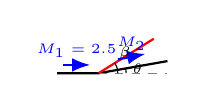
\begin{tikzpicture}[>=Latex,scale=0.35,baseline=(current bounding box.center)]
\draw[thick] (0,0) -- (1.5,0) -- (4,0.44);
\draw[dashed, gray] (1.5,0) -- (4,0);
\draw[red, thick] (1.5,0) -- (3.5,1.25);
\draw[->, blue, thick] (0.2,0.3) -- (1.2,0.3) node[above=-1pt, pos=0.5]{\fontsize{3.5}{4.5}\selectfont $M_1=2.5$};
\draw[->, blue, thick] (2.2,0.5) -- (3.2,0.7) node[above=-1.5pt, pos=0.5]{\fontsize{3.5}{4.5}\selectfont $M_2$};
\draw[thin] (2.5,0) arc (0:10:1.0) node[right=-1pt]{\fontsize{3.5}{4.5}\selectfont $\theta$};
\draw[thin] (2.2,0) arc (0:32:0.7) node[above right=-2pt]{\fontsize{3.5}{4.5}\selectfont $\beta$};
\end{tikzpicture}
\\
公式与计算链：
1. 确定激波角：由 $M_1 = 2.5, \theta = 10^\circ$ 查 $\theta-\beta-M$ 关系（或解方程）得弱斜激波解 $\beta \approx 31.85^\circ$。
2. 法向波前马赫数：$M_{n1} = M_1 \sin\beta = 2.5 \cdot \sin(31.85^\circ) = 1.319$。
3. 法向波后马赫数：$M_{n2} = \sqrt{\frac{1 + 0.2 M_{n1}^2}{1.4 M_{n1}^2 - 0.2}} = 0.776$。
4. 波后真实马赫数：$M_2 = \frac{M_{n2}}{\sin(\beta-\theta)} = \frac{0.776}{\sin(21.85^\circ)} = 2.086$。
5. 波后压力：$p_2 = p_1 \cdot \frac{7 M_{n1}^2 - 1}{6} = 85 \cdot 1.864 = 158.4$ kPa。
6. 波后温度：$\frac{\rho_2}{\rho_1} = \frac{6 M_{n1}^2}{M_{n1}^2 + 5} = 1.549 \Rightarrow T_2 = T_1 \frac{p_2/p_1}{\rho_2/\rho_1} = 298 \cdot 1.203 = 358.5$ K。

\subq{子题四：Prandtl-Meyer膨胀扇（凸角膨胀）流动计算}
超声速来流 $M_1 = 1.5$, 静压 $p_1 = 100$ kPa, 静温 $T_1 = 300$ K 绕折角 $\delta = 14.5^\circ$ 的凸角流动。试求波后马赫数 $M_2$, 压力 $p_2$ 及温度 $T_2$。\\
\hfill\begin{tikzpicture}[>=Latex,scale=0.35,baseline=(current bounding box.center)]
\draw[thick] (0,0.5) -- (1.5,0.5) -- (3.5,-0.02);
\draw[dashed, gray] (1.5,0.5) -- (3.5,0.5);
\foreach \a in {41.8, 33.0, 24.0, 15.5} {
  \draw[red, thin] (1.5,0.5) -- ++(\a:1.6);
}
\draw[->, blue, thick] (0.2,0.8) -- (1.2,0.8) node[above=-1.5pt, pos=0.5]{\fontsize{3.5}{4.5}\selectfont $M_1=1.5$};
\draw[->, blue, thick] (2.4,0.1) -- (3.4,-0.16) node[below=1pt, pos=0.5]{\fontsize{3.5}{4.5}\selectfont $M_2$};
\draw[thin] (2.2,0.5) arc (0:-14.5:0.7) node[right=1pt]{\fontsize{3.5}{4.5}\selectfont $\delta$};
\node[red] at (2.6, 1.4) {\fontsize{3.5}{4.5}\selectfont 膨胀扇};
\end{tikzpicture}
\\
公式与计算链：
1. 计算来流 PM 角度：$\nu_1 = \nu(M_1=1.5) = \sqrt{6}\tan^{-1}\sqrt{(1.5^2-1)/6} - \tan^{-1}\sqrt{1.5^2-1} \approx 11.9^\circ$。
2. 计算波后 PM 角度：$\nu_2 = \nu_1 + \delta = 11.9^\circ + 14.5^\circ = 26.4^\circ$。
3. 反求波后马赫数：由 $\nu_2 = 26.4^\circ$ 查表反解得 $M_2 = 2.0$。
4. 计算等熵波后压力：$p_2 = p_1 \left[ \frac{1+0.2M_1^2}{1+0.2M_2^2} \right]^{3.5} = 100 \cdot \left[ \frac{1.45}{1.80} \right]^{3.5} \approx 47.0$ kPa。
5. 计算等熵波后温度：$T_2 = T_1 \frac{1+0.2M_1^2}{1+0.2M_2^2} = 300 \cdot \frac{1.45}{1.80} \approx 241.7$ K。

\subq{子题五：Laval管外膨胀角与欠膨胀计算}
Laval喷管出口面积比 $A_e/A_t = 1.5$, 滞止压力 $p_0 = 500$ kPa, 背压 $p_b = 50$ kPa. 证明出口发生管外膨胀并求出口压力 $p_e$ 与膨胀角 $\Delta\nu$。\\
\hfill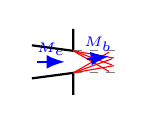
\begin{tikzpicture}[>=Latex,scale=0.35,baseline=(current bounding box.center)]
\draw[thick] (0,0.6) -- (1.5,0.4) -- (1.5,1.2);
\draw[thick] (0,-0.6) -- (1.5,-0.4) -- (1.5,-1.2);
\draw[dashed, gray] (1.5,0.4) -- (3,0.4);
\draw[dashed, gray] (1.5,-0.4) -- (3,-0.4);
\foreach \a in {-10, -20, -30} {
  \draw[red, thin] (1.5,0.4) -- ++(\a:1.5);
}
\foreach \a in {10, 20, 30} {
  \draw[red, thin] (1.5,-0.4) -- ++(\a:1.5);
}
\draw[->, blue, thick] (0.2,0) -- (1.2,0) node[above=-1.5pt, pos=0.5]{\fontsize{3.5}{4.5}\selectfont $M_e$};
\draw[->, blue, thick] (2.0,0.1) -- (2.8,0.2) node[above=-1.5pt, pos=0.5]{\fontsize{3.5}{4.5}\selectfont $M_b$};
\end{tikzpicture}
\\
公式与计算链：
1. 确定出口马赫数：由 $A_e/A^* = 1.5$ 查等熵超声速支得 $M_e = 1.86$。
2. 算出口压力：$p_e = p_0 (1 + 0.2 M_e^2)^{-3.5} = 500 \cdot (1 + 0.2 \cdot 1.86^2)^{-3.5} = 79.2$ kPa.
3. 判断欠膨胀：因为 $p_e = 79.2$ kPa $> p_b = 50$ kPa，所以出口发生欠膨胀，气流在出口外继续等熵膨胀。
4. 算最终马赫数：等熵 $p_{0b} = p_0 = 500$ kPa，由 $p_{0b}/p_b = 500/50 = 10 \Rightarrow (1+0.2M_b^2)^{3.5} = 10 \Rightarrow M_b = 2.157$。
5. 算膨胀角：$\Delta\nu = \nu(M_b) - \nu(M_e) = \nu(2.157) - \nu(1.86) = 30.88^\circ - 22.42^\circ = 8.46^\circ$。

\subq{子题六：超声速绕双凸极/接触面交汇计算}
\chap{母题5 粘性管流：N-S简化、层流解析、管路压损与小球沉降}
\mview{\key{母题总览}：看见黏度、管径、板距、流量、水头损失、粗糙度或小球沉降，判定为粘性流动。第一步：算雷诺数 $Re = Vd/\nu$ 判定层流（$Re < 2300$）或湍流（$Re > 4000$）。第二步：层流求解析速度分布（从简化 N-S 积分两次并用无滑移边界求常数）；湍流或管路计算求摩擦阻力（利用 Moody 图 $\lambda$ 或 $\lambda = 64/Re$ 算沿程与局部损失，并用能量方程联立）。}
\schemeviscous
\infoh{粘性管流信息库A 基础公式与简化原理}
* \key{牛顿剪切力与雷诺数}：$\tau = \mu \frac{du}{dy},\quad Re = \frac{Vd}{\nu} = \frac{\rho Vd}{\mu}$。水力直径：$d_h = \frac{4A}{\chi}$（$A$ 截面积，$\chi$ 润湿周长）。
* \key{N-S 方程简化（平行单向充分发展流）}：流向为 $x$，速度仅有 $u(y)$，惯性项全部消失，方程简化为：
  \[
  \mu \frac{d^2u}{dy^2} = \frac{dp}{dx} - \rho g_x = \frac{dp^*}{dx}\quad \text{(其中 } p^* = p + \rho gz \text{ 为广义压强，} z \text{ 轴向上为正)}
  \]
* \key{Hagen-Poiseuille 圆管层流}：速度分布为抛物线 $u(r) = U_{\max}(1 - r^2/R^2)$，其中 $U_{\max} = 2V$。
  \[
  Q = \frac{\pi d^4 \Delta p}{128\mu L},\quad \Delta p = \frac{32\mu LV}{d^2},\quad \lambda = \frac{64}{Re},\quad \tau_w = \frac{d\Delta p}{4L} = \frac{8\mu V}{d}
  \]
* \key{管路水头损失}：沿程损失 $h_f = \lambda \frac{L}{d} \frac{V^2}{2g}$，局部损失 $h_{\zeta} = \zeta \frac{V^2}{2g}$。完全粗糙管阻力与 $Re$ 无关，只取决于相对粗糙度 $\varepsilon/d$。
* \key{Stokes 低雷诺数阻力}：若 $Re = \frac{\rho Ud}{\mu} < 1$，球形颗粒受阻力 $D = 3\pi \mu d U$，阻力系数 $C_D = 24/Re$。

\infoh{粘性管流信息库B 常见概念与常考判断}
* \key{完全发展流动}：圆管充分发展流动中，速度分布沿轴向不变（$\partial u/\partial x = 0$），压强梯度为常数（$dp/dx = C$），沿程损失反映壁面摩阻。
* \key{湍流壁律分区}：摩擦速度 $u_\tau = \sqrt{\tau_w/\rho}$，无量纲高度 $y^+ = y u_\tau/\nu$。粘性底层（$y^+ < 5$，粘性主导，速度线性分布）、过渡缓冲层（$5 \le y^+ \le 30$）、对数律区（$y^+ > 30$，湍流剪切主导）。
* \key{雷诺应力与混合长度}：雷诺应力 $-\rho \overline{u'v'}$ 源于湍流脉动的动量输运；总剪应力为分子粘性剪应力与雷诺剪应力之和。混合长度假设 $\tau_t = \rho l^2 |du/dy| (du/dy)$，近壁 $l = \kappa y$。
* \key{数值模拟方法}：DNS（直接解 N-S，解析全尺度，最贵）；LES（解析大涡，模型化小涡）；RANS（雷诺时均，对雷诺应力建模，最常用）。

\infoh{粘性管流信息库C 解题食谱与步骤（一步步带入指导）}

\subq{平板 Couette 流（纯剪切流）：已知上板速 U、板距 h、黏度 $\mu$，求速度、流量和剪力}
1. \key{写速度分布}：直接带入线性公式：$u(y) = U \frac{y}{h}$（$y=0$ 为下板，$y=h$ 为上板）。
2. \key{求单位宽度流量 $q$}：$q = \int_0^h u\,dy = \frac{1}{2} U h$。若已知板宽 $b$，总流量 $Q = q b = \frac{1}{2} U h b$。
3. \key{求壁面剪应力}：由牛顿内摩擦定律，全场剪应力恒定：$\tau = \mu \frac{du}{dy} = \mu \frac{U}{h}$。壁面受力 $F = \tau A = \mu \frac{U}{h} A$。

\subq{平板 Poiseuille 流（压差流）：已知两固定板距 h、压降 $\Delta p/L$（或 $dp/dx$）、黏度 $\mu$，求速度分布与流量}
1. \key{求速度分布}：直接带入抛物线公式：$u(y) = \frac{1}{2\mu} \left( -\frac{dp}{dx} \right) y (h-y)$，其中 $-\frac{dp}{dx} = \frac{\Delta p}{L}$。
2. \key{求最大速度}：在中心线 $y = h/2$ 处速度最大：$u_{\max} = \frac{h^2}{8\mu} \left( -\frac{dp}{dx} \right)$。
3. \key{求平均速度与单位宽流量}：平均速度 $\bar{u} = \frac{2}{3}u_{\max}$；单位宽度流量 $q = \bar{u}h = \frac{h^3}{12\mu} \left( -\frac{dp}{dx} \right)$。
4. \key{求壁面剪应力}：代入 $y=0$ 得壁剪应力大小 $\tau_w = \frac{h}{2} \left( -\frac{dp}{dx} \right)$。

\subq{平板 Couette-Poiseuille 结合流：已知上板速 U、板距 h、压降 $dp/dx$、黏度 $\mu$，求流速最大值和壁面受力}
1. \key{写出叠加速度公式}：$u(y) = U \frac{y}{h} + \frac{1}{2\mu} \left( -\frac{dp}{dx} \right) y (h-y)$。
2. \key{求最大流速位置}：对 $y$ 求导并令其为 $0$：$\frac{du}{dy} = \frac{U}{h} + \frac{1}{2\mu} \left( -\frac{dp}{dx} \right) (h-2y) = 0$，解出 $y_m = \frac{h}{2} + \frac{\mu U}{h(-dp/dx)}$。若 $y_m \in [0, h]$，则最大速度为 $u(y_m)$。
3. \key{求流量}：叠加两项的流量：$q = \frac{1}{2}Uh + \frac{h^3}{12\mu}\left(-\frac{dp}{dx}\right)$。
4. \key{求壁面剪力}：求导算剪应力分布 $\tau(y) = \mu \frac{du}{dy} = \mu \frac{U}{h} + \frac{1}{2}\left(-\frac{dp}{dx}\right)(h-2y)$。代入下壁 $y=0$ 得 $\tau_1 = \mu \frac{U}{h} + \frac{h}{2}\left(-\frac{dp}{dx}\right)$；代入上壁 $y=h$ 得 $\tau_2 = \mu \frac{U}{h} - \frac{h}{2}\left(-\frac{dp}{dx}\right)$。

\subq{两层流体剪切流动：已知厚度 $h_1,h_2$、黏度 $\mu_1,\mu_2$、上板速 U，求剪应力与界面速度}
1. \key{求全场恒定剪应力 $\tau$}：阻力串联：$\tau = \frac{U}{h_1/\mu_1 + h_2/\mu_2} = \frac{U \mu_1 \mu_2}{\mu_2 h_1 + \mu_1 h_2}$。
2. \key{求交界面速度 $U_i$}：代入下层：$U_i = \tau \frac{h_1}{\mu_1} = U \frac{\mu_2 h_1}{\mu_2 h_1 + \mu_1 h_2}$。
3. \key{写出分段速度分布}：下层（$0\le y \le h_1$）：$u_1(y) = \tau \frac{y}{\mu_1}$；上层（$h_1 \le y \le h_1+h_2$）：$u_2(y) = U_i + \tau \frac{y-h_1}{\mu_2}$。

\subq{倾斜平板重力流（如液膜下落）：已知倾角 $\theta$、液膜厚 H、黏度 $\mu$、密度 $\rho$，求速度分布与流量}
1. \key{建立微分方程并积分两次}：沿壁面单向重力流（无压差）：$\mu \frac{d^2u}{dy^2} + \rho g \sin\theta = 0 \Rightarrow u(y) = -\frac{\rho g \sin\theta}{2\mu} y^2 + C_1 y + C_2$。
2. \key{代入边界条件求常数}：
   * 在壁面 $y=0$ 无滑移：$u(0) = 0 \Rightarrow C_2 = 0$。
   * 在液膜自由表面 $y=H$ 无剪力：$\left.\frac{du}{dy}\right|_{y=H} = 0 \Rightarrow -\frac{\rho g \sin\theta}{\mu} H + C_1 = 0 \Rightarrow C_1 = \frac{\rho g \sin\theta}{\mu} H$。
3. \key{代回整理速度与流量}：速度为 $u(y) = \frac{\rho g \sin\theta}{\mu} \left( Hy - \frac{1}{2}y^2 \right)$。积分求单位宽流量 $q = \int_0^H u\,dy = \frac{\rho g \sin\theta\,H^3}{3\mu}$。

\subq{子题：Hagen-Poiseuille 圆管层流计算}
输送 SAE 30 机油 ($\rho = 888$ kg/m$^3$, $\mu = 0.29$ Pa$\cdot$s) 的圆管长 $L=100$ m, 直径 $d=50$ mm, 流量 $Q = 1.2$ L/s ($0.0012$ m$^3$/s). 试验证流动状态，并计算沿程压降 $\Delta p$ 与管壁剪应力 $\tau_w$。\\
公式与计算链：
1. 验证流态：平均流速 $V = \frac{4Q}{\pi d^2} = 0.611$ m/s.
   雷诺数 $Re = \frac{\rho V d}{\mu} = \frac{888 \cdot 0.611 \cdot 0.05}{0.29} = 93.6 < 2300$, 确为层流。
2. 计算沿程压降：
   $\Delta p = \frac{128 \mu L Q}{\pi d^4} = \frac{128 \cdot 0.29 \cdot 100 \cdot 0.0012}{\pi \cdot 0.05^4} = 226.9$ kPa.
3. 计算壁面剪应力：
   $\tau_w = \frac{d\Delta p}{4L} = \frac{0.05 \cdot 226860}{400} = 28.36$ Pa.
   (或由剪切力公式 $\tau_w = \frac{8\mu V}{d} = 28.36$ Pa).

\subq{小球低雷诺数沉降：已知球径 d、小球密度 $\rho_s$、流体密度 $\rho$ 与黏度 $\mu$，求沉降终速}
1. \key{列受力平衡求终速}：匀速下落时重力 - 浮力 = 阻力：$(\rho_s - \rho) g \frac{\pi d^3}{6} = 3\pi \mu d U_t \Rightarrow U_t = \frac{(\rho_s - \rho) g d^2}{18\mu}$。
2. \key{带入验证雷诺数}：算出 $U_t$ 后，必须带入验证 $Re = \frac{\rho U_t d}{\mu}$。若 $Re < 1$ 则公式成立，沉降速度确为 $U_t$；若 $Re > 1$，则必须用阻力系数 $C_D$ 查图迭代。

\subq{圆管湍流近壁三层厚度计算：已知管径 d、平均流速 V、黏度 $\nu$，求粘性底层和缓冲层厚度}
1. \key{求摩擦速度 $u_\tau$}：代入并迭代求解方程：$\frac{V}{u_\tau} = 2.5 \ln\left( \frac{R u_\tau}{\nu} \right) + 1.75$（其中 $R = d/2$），解出 $u_\tau$。
2. \key{计算粘性底层厚度 $y_{\text{sub}}$}：令 $y^+ = 5 \Rightarrow y_{\text{sub}} = \frac{5\nu}{u_\tau}$。
3. \key{计算缓冲层外缘厚度 $y_{\text{buf}}$}：令 $y^+ = 30 \Rightarrow y_{\text{buf}} = \frac{30\nu}{u_\tau}$。

\subq{汽蚀与泵最大安装高度：已知泵流量 Q、吸水管长 L、管径 d、摩擦阻力、大气压 $p_a$ 和汽化压 $p_v$，求最大高度 h}
1. \key{求流速与阻力系数}：$V = \frac{4Q}{\pi d^2}$，由 $Re = \frac{Vd}{\nu}$ 和 $\varepsilon/d$ 确定沿程阻力系数 $\lambda$。
2. \key{计算总水头损失}：沿程水头损失 $h_f = \lambda \frac{L}{d}\frac{V^2}{2g}$，局部水头损失 $h_{\zeta} = \sum \zeta \frac{V^2}{2g}$。
3. \key{列能量方程并带入临界汽蚀限制}：从吸水池面 $1$ 到泵入口 $2$ 列能量方程，令泵入口压强 $p_2 \ge p_v + \Delta p_{\text{safe}}$（不给安全余量时默认为 $p_v$）：
   \[
   z_1 + \frac{p_a}{\rho g} + 0 = z_2 + \frac{p_2}{\rho g} + \frac{V^2}{2g} + h_f + h_{\zeta} \Rightarrow h = z_2 - z_1 \le \frac{p_a - p_v}{\rho g} - \frac{V^2}{2g} - h_f - h_{\zeta}
   \]

\chap{母题6 边界层、外绕流阻力、综合相似}
\mview{\key{母题总览}：看见平板外流、$\delta,C_f,C_D$、阻力、分离、模型试验，用边界层/外绕/相似。首写$Re_x/Re_L$或$\pi$群。顺序：判层湍$\to \delta,C_f\to D$；相似先选主导准则。检查：湿面积/迎风面积、局部/平均系数、逆压梯度分离。}
\schemebl
\infoh{边界层/外绕信息库A 基础公式和数学运算}
\fmlb{\begin{aligned}
&Re_x = Ux/\nu,\quad Re_L = UL/\nu,\quad D/Dt = \partial_t + u\partial_x + v\partial_y + w\partial_z\\
&\text{Prandtl控制方程：} u_x+v_y=0,\quad uu_x+vu_y=\nu u_{yy},\quad p_y=0\\
&\text{层流Blasius：} \delta=5x/\sqrt{Re_x},\quad c_f=0.664/\sqrt{Re_x},\quad \bar C_f=1.328/\sqrt{Re_L}\\
&\text{湍流平板：} \delta=0.37x/Re_x^{1/5},\quad \bar C_f=0.074/Re_L^{1/5}\\
&\text{转捩修正：} \bar C_f=0.074/Re_L^{1/5}-1742/Re_L \quad (\text{临界 } Re_{cr}=5\times 10^5)\\
&\text{排挤厚度：} \delta^* = \int_0^\delta (1-u/U) dy,\quad \text{动量厚度：} \theta = \int_0^\delta \frac{u}{U}(1-u/U) dy\\
&\text{Von Karman积分：} \tau_w = \rho U^2 \frac{d\theta}{dx},\quad \tau_w = \mu \left(\frac{\partial u}{\partial y}\right)_{y=0}\\
&\text{阻力/功率：} D = \bar C_f \cdot \frac{1}{2}\rho U^2 A \quad (\text{双面 } A=2Lb),\quad P = DU\\
&\text{Stokes小球阻力：} D = 3\pi \mu d U = 6\pi \mu a U \quad (Re<1,\ d=2a)\\
&\text{钝体外绕阻力：} D = C_D \cdot \frac{1}{2}\rho U^2 A \quad (A \text{ 为迎风面积 }\pi d^2/4)
\end{aligned}}

\infoh{边界层/外绕信息库B 证明链与判定链}
* \key{平板边界层流程}：求 $Re_L = UL/\nu$ $\to$ 对比 $Re_{cr}$ 判层/湍/转捩 $\to$ 选 $\bar C_f, \delta(L)$ $\to$ 摩擦力 $D = \bar C_f \frac{1}{2}\rho U^2 A$ （单双面） $\to$ 功率 $P=DU$。
* \key{动量积分法推导}：给剖面 $u/U=f(\eta)$，令 $\eta=y/\delta \Rightarrow dy=\delta d\eta$ $\to$ 积分求比值 $\delta^*/\delta = \int_0^1(1-f)d\eta$, $\theta/\delta = \int_0^1 f(1-f)d\eta$ $\to$ 由 $\tau_w = \mu (\partial u/\partial y)_0 = \rho U^2 d\theta/dx$ 列关于 $\delta(x)$ 的微分方程并求解。
* \key{相似与量纲分析}：确定变量数 $n$ 与基本量纲数 $r \Rightarrow \pi$ 群数为 $n-r$ $\to$ 选择 $\rho, V, L$ 为重复变量，其余变量 $X$ 组成 $\pi = X \rho^a V^b L^c$ 解指数。重力主导用 Froude 相似 ($Fr$)，粘性主导用 Reynolds 相似 ($Re$)。

\infoh{边界层/外绕信息库C 常见结论与答题句}
* \key{分离答题句}：因逆压梯度 $dp/dx>0$ 使近壁流体减速，壁面速度梯度 $\partial u/\partial y|_w$ 降至零并反向，边界层发生分离。尾流区压强骤降导致压差阻力急剧增大。
* \key{位移与动量厚度意义}：排挤厚度 $\delta^*$ 表示由于边界层粘性减速导致主流等效外移的距离；动量厚度 $\theta$ 表示边界层内动量亏损的折算厚度。
* \key{流线型与钝体阻力}：流线型物体以壁面剪切摩擦阻力为主，钝体以分离后的压差阻力为主。高 $Re$ 时物面外部可近似为无粘势流，靠壁层必须用边界层方程。

\infoh{边界层/外绕信息库D 易错检查}
* $x$ 必须从板前缘起算，问板尾厚度取 $x=L$。
* 局部摩擦系数 $c_f$ 只用于计算局部剪切应力，求整板阻力必须用平均系数 $\bar C_f$。
* 迎风面积 $A_{\rm front}$ 用于球/圆柱等外绕阻力，湿面积 $A_{\rm wet}$ 用于平板摩擦。
* 火车等车速 $160$ km/h 等必须换算为 $m/s$。

\subq{子题六：平板层流边界层计算（Blasius）}
作业代表题：10.2 平板层流油流。原题：油 $\mu = 0.731$ Pa·s, $\rho = 925$ kg/m$^3$, 流速 $U = 0.6$ m/s, 板长 $L = 0.5$ m, 宽 $b = 0.15$ m, 求最大边界层厚度 $\delta_{\max}$ 和双面摩擦阻力 $D$。\\
公式链：
1. 运动粘度 $\nu = \mu/\rho = 7.90 \times 10^{-4}$ m$^2$/s。
2. 板尾雷诺数 $Re_L = UL/\nu = 3.80 \times 10^2$。由于 $Re_L \ll 5 \times 10^5$，全板为层流。
3. 板尾厚度 $\delta_{\max} = 5L / \sqrt{Re_L} = 5 \times 0.5 / \sqrt{380} = 0.128$ m。
4. 平均摩阻系数 $\bar C_f = 1.328 / \sqrt{Re_L} = 0.0682$。
5. 双面阻力面积 $A = 2Lb = 0.15$ m$^2$。
6. 总摩擦阻力 $D = \bar C_f \cdot \frac{1}{2}\rho U^2 \cdot A = 0.0682 \cdot 0.5 \cdot 925 \cdot 0.6^2 \cdot 0.15 = 1.70$ N。

\subq{子题七：平板湍流与混合转捩边界层计算}
作业代表题：10.10 火车摩擦阻力。原题：流线型火车长 $L=110$ m, 周长 $b=8.25$ m, 速度 $U=160$ km/h, 空气 $\rho=1.22$ kg/m$^3$, $\mu=1.79\times10^{-5}$ Pa·s, 临界雷诺数 $Re_{cr}=5\times10^5$, 求层流维持长度 $x_{cr}$ 和克服阻力所需功率 $P$。\\
公式链：
1. 流速换算 $U = 160 / 3.6 = 44.44$ m/s。单面受湿面积 $S = Lb = 907.5$ m$^2$。
2. 临界长度 $x_{cr} = Re_{cr} \mu / (\rho U) = 5\times 10^5 \cdot 1.79\times 10^{-5} / (1.22 \cdot 44.44) = 0.165$ m。
3. 全板雷诺数 $Re_L = \rho UL / \mu = 1.22 \cdot 44.44 \cdot 110 / (1.79 \times 10^{-5}) = 3.33 \times 10^8$。
4. 由于 $Re_L > Re_{cr}$，采用转捩修正摩阻系数：$\bar C_f = \frac{0.074}{Re_L^{1/5}} - \frac{1742}{Re_L} = \frac{0.074}{(3.33 \times 10^8)^{0.2}} - \frac{1742}{3.33 \times 10^8} = 0.00146$。
5. 摩擦阻力 $D = \bar C_f \cdot \frac{1}{2}\rho U^2 S = 0.00146 \cdot 0.5 \cdot 1.22 \cdot 44.44^2 \cdot 907.5 = 1.59 \times 10^3$ N。
6. 克服阻力功率 $P = DU = 1.59 \times 10^3 \cdot 44.44 = 70.8$ kW。

\subq{子题八：给速度分布剖面求位移厚度与动量损失厚度}
作业代表题：10.3 剖面厚度计算。原题：已知边界层速度分布剖面为抛物线型 $\frac{u}{U} = 2\eta - \eta^2$（其中 $\eta = y/\delta$），求排挤厚度 $\delta^*$、动量损失厚度 $\theta$ 和形状系数 $H$。\\
公式链：
1. 引入无量纲自变量 $\eta = y/\delta$，则 $dy = \delta d\eta$。
2. 排挤厚度 $\delta^* = \int_0^\delta (1 - \frac{u}{U}) dy = \delta \int_0^1 (1 - 2\eta + \eta^2) d\eta = \delta [ \eta - \eta^2 + \frac{\eta^3}{3} ]_0^1 = \frac{1}{3}\delta$。
3. 动量损失厚度 $\theta = \int_0^\delta \frac{u}{U}(1 - \frac{u}{U}) dy = \delta \int_0^1 (2\eta - \eta^2)(1 - 2\eta + \eta^2) d\eta = \delta \int_0^1 (2\eta - 5\eta^2 + 4\eta^3 - \eta^4) d\eta = \delta [ \eta^2 - \frac{5}{3}\eta^3 + \eta^4 - \frac{\eta^5}{5} ]_0^1 = \frac{2}{15}\delta$。
4. 形状系数 $H = \delta^* / \theta = (1/3) / (2/15) = 2.50$。

\subq{子题九：任意剖面的动量积分推导与板阻力求法}
作业代表题：10.5 正弦剖面积分。原题：假设层流剖面为 $\frac{u}{U_e} = a + b\sin(cy/\delta)$。由边界条件确定常数，并求位移厚度、动量厚度及总阻力系数 $C_D$。\\
公式链：
1. 边界条件定常数：壁面无滑移 $u(0)=0 \Rightarrow a = 0$；外缘速度等于外流 $u(\delta)=U_e \Rightarrow b\sin(c) = 1$；外缘速度平滑连接 $\frac{\partial u}{\partial y}|_{y=\delta}=0 \Rightarrow bc\cos(c)=0 \Rightarrow c = \pi/2, b = 1$。即 $\frac{u}{U_e} = \sin(\frac{\pi\eta}{2})$。
2. 积分计算厚度比值：$\delta^* = \delta \int_0^1 (1 - \sin\frac{\pi\eta}{2}) d\eta = \delta(1 - 2/\pi)$，$\theta = \delta \int_0^1 \sin\frac{\pi\eta}{2}(1 - \sin\frac{\pi\eta}{2}) d\eta = \delta(2/\pi - 1/2)$。比值 $\delta^*/\theta = 2.66$。
3. 壁面剪应力 $\tau_w = \mu \frac{\partial u}{\partial y}|_{y=0} = \mu U_e \frac{\pi}{2\delta}$。
4. 代入动量积分方程 $\tau_w = \rho U_e^2 \frac{d\theta}{dx}$ （令 $\theta = A\delta$, $A = 2/\pi - 1/2 = 0.1366$）：
   $\mu U_e \frac{\pi}{2\delta} = \rho U_e^2 A \frac{d\delta}{dx} \Rightarrow \delta \frac{d\delta}{dx} = \frac{\pi \nu}{2A U_e}$。
5. 积分并代入 $\delta(0)=0$：$\delta(x) = \sqrt{\frac{\pi \nu x}{A U_e}}$。在尾缘 $x=L$：$\theta(L) = A \delta(L) = \sqrt{A \pi \nu L / U_e}$。
6. 单面总摩擦阻力 $D = \rho U_e^2 \theta(L)$。总阻力系数 $C_D = \frac{D}{\frac{1}{2}\rho U_e^2 L} = \frac{2\theta(L)}{L} = 2\sqrt{\frac{A\pi}{Re_L}} = 2\sqrt{0.1366\pi} / \sqrt{Re_L} = 1.31 / \sqrt{Re_L}$。

\subq{子题十：利用 Buckingham $\pi$ 定理推出无量纲关系式}
作业代表题：11.5 阻力公式推出。原题：水下航行器所受流体阻力 $F$ 与长度 $L$, 流速 $V$, 流体密度 $\rho$, 动力粘度 $\mu$ 和重力加速度 $g$ 有关。试推求 $F$ 的无量纲关系式。\\
公式链：
1. 列表写变量与量纲：$F [M L T^{-2}]$, $L [L]$, $V [L T^{-1}]$, $\rho [M L^{-3}]$, $\mu [M L^{-1} T^{-1}]$, $g [L T^{-2}]$。变量数 $n = 6$，基本量纲数 $r = 3$。独立 $\pi$ 数为 $n-r = 3$ 个。
2. 选取重复变量 $\rho, V, L$（必须包含所有基本量纲，且量纲独立，不能含被求量 $F$）。
3. 建立并求解 $\pi$ 方程：
   - 对于 $F$：令 $\pi_1 = F \rho^a V^b L^c \Rightarrow [M^0 L^0 T^0] = [M L T^{-2}] [M^a L^{-3a}] [L^b T^{-b}] [L^c] \Rightarrow a=-1, b=-2, c=-2 \Rightarrow \pi_1 = \frac{F}{\rho V^2 L^2}$。
   - 对于 $\mu$：令 $\pi_2 = \mu \rho^a V^b L^c \Rightarrow \text{同理求得 } a=-1, b=-1, c=-1 \Rightarrow \pi_2 = \frac{\mu}{\rho V L} = \frac{1}{Re}$。
   - 对于 $g$：令 $\pi_3 = g \rho^a V^b L^c \Rightarrow \text{同理求得 } a=0, b=-2, c=1 \Rightarrow \pi_3 = \frac{gL}{V^2} = \frac{1}{Fr^2}$。
4. 综合关系式 $\Phi(\pi_1, \pi_2, \pi_3) = 0 \Rightarrow \frac{F}{\rho V^2 L^2} = \phi(Re, Fr)$，即 $F = \rho V^2 L^2 \phi(Re, Fr)$。

\subq{子题十一：模型相似与动力学换算计算}
作业代表题：11.7 模型换算。原题：船只模型比例尺 $\lambda_l = L_m/L_p = 1/25$，原型设计航速 $V_p = 10$ m/s。若重力波阻力占主导（按 $Fr$ 相似），求模型航速 $V_m$ and 测得阻力 $F_m = 10$ N 时原型对应的阻力 $F_p$（设海水密度 $\rho_p = 1025$, 淡水 $\rho_m = 1000$）。\\
公式链：
1. 重力波主导采用 Froude 相似：$Fr_m = Fr_p \Rightarrow \frac{V_m}{\sqrt{g L_m}} = \frac{V_p}{\sqrt{g L_p}}$。
2. 速度比例换算：$V_r = \frac{V_m}{V_p} = \sqrt{\frac{L_m}{L_p}} = \sqrt{\lambda_l} = \frac{1}{5}$。则模型航速 $V_m = V_p \cdot V_r = 10 \cdot 0.2 = 2.0$ m/s。
3. 阻力比例换算（动力相似）：$F_r = \frac{F_m}{F_p} = \rho_r V_r^2 L_r^2 = \frac{\rho_m}{\rho_p} \cdot V_r^2 \cdot \lambda_l^2$。
4. 阻力值求解：$F_p = F_m \cdot \frac{\rho_p}{\rho_m} \cdot \frac{1}{V_r^2} \cdot \frac{1}{\lambda_l^2} = 10 \cdot \frac{1025}{1000} \cdot 5^2 \cdot 25^2 = 10 \cdot 1.025 \cdot 25 \cdot 625 = 1.60 \times 10^5$ N。
5. 若粘性占主导（雷诺相似且使用同种流体），则速度比 $V_r = 1/\lambda_l = 25$，原型流速 $V_p = 10$ m/s 时模型速度须达 $250$ m/s，通常发生 Re 与 Fr 冲突。

\subq{子题十二：管路水击（水锤）压强计算}
作业代表题：书8.15 阀门水击。原题：长 $L=1000$ m 的钢管，水流速 $V_0=2.0$ m/s，水击波速 $a=1000$ m/s，若阀门在 $T=0.5$ s 内完全关闭，求最大水击压强 $\Delta p_{\max}$，若关闭时间为 $T=3.0$ s 呢？\\
公式链：
1. 计算水击波往返时间：$T_0 = \frac{2L}{a} = \frac{2 \times 1000}{1000} = 2.0$ s。
2. 阀门快速关闭（$T = 0.5$ s $< T_0 = 2.0$ s）：属于直接（直接/快速）水击。
   最大水击压力上升：$\Delta p_{\max} = \rho a V_0 = 1000 \cdot 1000 \cdot 2.0 = 2.0 \times 10^6$ Pa $= 2.0$ MPa。
3. 阀门缓慢关闭（$T = 3.0$ s $> T_0 = 2.0$ s）：属于间接（间接/缓慢）水击。
   最大水击压力上升：$\Delta p_{\max}' = \rho a V_0 \cdot \frac{T_0}{T} = 2.0\text{ MPa} \cdot \frac{2.0}{3.0} = 1.33$ MPa。

\subq{子题十三：明渠均匀流流量与流速计算}
作业代表题：明渠均匀流。原题：一矩形渠道宽 $b=4$ m, 水深 $h=2$ m, 底坡 $i=0.001$, Manning粗糙系数 $n=0.02$, 求通过渠道的体积流量 $Q$。\\
公式链：
1. 渠道截面积：$A = b \cdot h = 4 \times 2 = 8$ m$^2$。
2. 湿周：$\chi = b + 2h = 4 + 2 \times 2 = 8$ m。
3. 水力半径：$R = A / \chi = 8 / 8 = 1.0$ m。
4. 谢才系数（Manning公式）：$C = \frac{1}{n} R^{1/6} = \frac{1}{0.02} \cdot 1.0^{1/6} = 50.0$ m$^{1/2}$/s。
5. 平均流速：$V = C \sqrt{R i} = 50.0 \times \sqrt{1.0 \times 0.001} = 1.58$ m/s。
6. 体积流量：$Q = A \cdot V = 8 \times 1.58 = 12.65$ m$^3$/s。

\chap{母题7 场变量、应力张量、静水压与证明小题}
\mview{\key{母题定位}：看见速度场$u,v,w$、应力张量$P$、给定平面法向$\bm n$、闸门/曲面/浮体、或“证明存在势函数/流函数/伯努利条件”，归到本母题。先判模型，再写最短公式链。}
\infoh{场变量信息库A 基础公式和数学运算}
梯度$\nabla f=(f_x,f_y,f_z)$；散度$\nabla\cdot\bm V=u_x+v_y+w_z$；旋度$\nabla\times\bm V=(w_y-v_z,\ u_z-w_x,\ v_x-u_y)$。二维旋度$\Omega_z=v_x-u_y$，角速度$\omega_z=\Omega_z/2$。材料导数$D/Dt=\partial_t+u\partial_x+v\partial_y+w\partial_z$；$a_x=u_t+uu_x+vu_y+wu_z$，其余分量同理。柱坐标常用：$\nabla\cdot\bm V=\frac1r\partial(rv_r)/\partial r+\frac1r\partial v_\theta/\partial\theta+\partial v_z/\partial z$。
\infoh{场变量信息库B 证明链和判定链}
不可压判定：$\nabla\cdot\bm V=0$；二维不可压可令$u=\psi_y,\ v=-\psi_x$。无旋判定：$\nabla\times\bm V=0$；无旋可令$\bm V=\nabla\phi$。势流满足$\nabla^2\phi=0$，二维不可压流函数满足$\nabla^2\psi=-\Omega_z$，无旋时$\nabla^2\psi=0$。Bernoulli从Euler沿流线积分；定常、不可压、无粘、保守体力下沿流线成立，无旋时可全场用。
\infoh{场变量信息库C 常见结论库}
点涡$v_\theta=\Gamma/(2\pi r)$，原点外无旋但环量非零；强迫涡$v_\theta=\omega r$，$\Omega_z=2\omega$，自由面$z=\omega^2r^2/(2g)+C$；自由涡$v_\theta=C/r$，$p/\rho+\frac12v^2+gz=C$。平面方程$F=0$的单位法向$\bm n=\pm\nabla F/|\nabla F|$；圆柱面$y^2+z^2=R^2$法向$(0,y/R,z/R)$。
\infoh{场变量信息库D 易错检查}
应力张量题不是直接取矩阵元素，必须先算$\bm t_n=P\bm n$。流线不是迹线：定常时可同，非定常通常不同。二维不可压不等于无旋；有$\psi$不代表有$\phi$。证明题要先写适用条件，不能只抄结论。
\conceptq{母题7高频证明句}
应力张量对称：无体偶力时微元角动量平衡，故 $p_{xy}=p_{yx}$ 等，独立分量由 9 个变 6 个。\\
Laplace来源：不可压 $\nabla\cdot\bm V=0$ 且无旋 $\bm V=\nabla\phi$，故 $\nabla^2\phi=0$；二维流函数有 $\nabla^2\psi=-\Omega_z$。\\
Bernoulli沿流线：由 Euler 方程沿流线积分；若还无旋，则积分常数全场相同。\\
压力中心低于形心：静水压随深度增大，下部压力权重大，所以合力作用点比形心深。

\subq{子题一：三维应力张量与任意平面上的应力分析}
作业代表题：应力张量。原题：已知某流场中一点处的应力张量为 $P = \begin{pmatrix} 2 & 1 & 0 \\ 1 & -3 & 2 \\ 0 & 2 & 1 \end{pmatrix}$ kPa，求通过该点且平行于平面 $x+y+z=0$ 的平面上的应力矢量、法向应力、切向应力及应力矢量与法线的夹角。\\
公式链：
1. 求单位法向量：由平面方程得 $\bm n = \frac{1}{\sqrt{3}}(1, 1, 1)^T$。
2. 计算应力矢量：$\bm t_n = P \bm n = \frac{1}{\sqrt{3}} \begin{pmatrix} 2&1&0\\1&-3&2\\0&2&1 \end{pmatrix} \begin{pmatrix} 1\\1\\1 \end{pmatrix} = \begin{pmatrix} \sqrt{3} \\ 0 \\ \sqrt{3} \end{pmatrix}$ kPa，大小 $|\bm t_n| = \sqrt{6}$ kPa。
3. 计算法向应力：$\sigma_n = \bm t_n \cdot \bm n = 2$ kPa（拉应力）。
4. 计算切向应力大小：$\tau = \sqrt{|\bm t_n|^2 - \sigma_n^2} = \sqrt{6 - 4} = \sqrt{2}$ kPa $\approx 1.414$ kPa。
5. 计算夹角：$\cos\alpha = \sigma_n / |\bm t_n| = 2/\sqrt{6} = \sqrt{2/3} \Rightarrow \alpha = 35.26^\circ$。

\subq{子题二：速度场运动学性质判定（连续、有旋、流线与迹线）}
作业代表题：流线与迹线。原题：已知二维流场速度为 $u=x/(1+t)$，$v=y$，求：(1) $t=0$ 时通过 $(1,1)$ 的流线；(2) $t=0$ 时刻从 $(1,1)$ 出发的迹线。\\
公式链：
1. 连续性与有旋性判定：$\nabla\cdot\bm V = u_x+v_y = 1/(1+t) + 1 \ne 0$（可压）；$\Omega_z = v_x-u_y = 0$（无旋）。
2. 计算 $t=0$ 时的流线：代入 $t=0$ 得 $u=x, v=y$。流线微分方程 $dy/dx = v/u = y/x \Rightarrow y = Cx$。过 $(1,1)$ 得 $y = x$。
3. 计算迹线：迹线微分方程 $dx/dt = u = x/(1+t) \Rightarrow x(t) = C_1(1+t)$；$dy/dt = v = y \Rightarrow y(t) = C_2 e^t$。
4. 带入初始条件：$t=0$ 时 $x=1, y=1 \Rightarrow C_1=1, C_2=1$。消去参量 $t$：$t = x-1 \Rightarrow y = e^{x-1}$。

\subq{子题三：平面静水总压力与铰链力矩计算}
作业代表题：倾斜闸门。原题：一矩形闸门宽 $b=2$ m，高 $h=3$ m，与水平面夹角 $\theta=45^\circ$，顶端位于水深 $h_0=1$ m 处。求闸门所受静水总压力 $F$ 及压力中心 $y_D$，若顶端设铰链，求底端开启所需的拉力 $T$。\\
公式链：
1. 沿板坐标形心位置：顶端 inclined 坐标 $y_0 = h_0 / \sin 45^\circ = 1.414$ m，形心 $y_C = y_0 + h/2 = 2.914$ m。
2. 计算形心深度：$h_C = y_C \sin 45^\circ = 2.06$ m。
3. 计算总压力：$F = \rho g h_C A = 1000 \times 9.8 \times 2.06 \times (2\times 3) = 121.1$ kN。
4. 压力中心：$y_D = y_C + \frac{I_C}{y_C A} = 2.914 + \frac{2 \times 3^3 / 12}{2.914 \times 6} = 3.171$ m。与顶端距离 $d = y_D - y_0 = 1.757$ m。
5. 开启力矩平衡：以铰点求矩 $F \cdot d = T \cdot h \Rightarrow T = 121.1 \times 1.757 / 3 = 70.9$ kN。

\subq{子题四：曲面静水总压力计算（水平与竖直分量）}
作业代表题：圆弧闸门。原题：一半径 $R=1$ m，长 $L=2$ m 的四分之一圆弧闸门，水深 $H=2$ m（刚好淹没圆弧顶）。求闸门所受的水平分力 $F_H$、竖直分力 $F_V$ 及合力 $F$。\\
公式链：
1. 水平分力：投影面高 $h_y=R=1$ m，形心深 $h_C = H - R/2 = 1.5$ m。$F_H = \rho g h_C (R L) = 1000 \times 9.8 \times 1.5 \times 2 = 29.4$ kN。
2. 竖直分力：压力体体积 $V = L \cdot (H \cdot R - \frac{1}{4}\pi R^2) = 2 \times (2 - 0.785) = 2.43$ m$^3$。$F_V = \rho g V = 23.8$ kN（方向向上）。
3. 合力及夹角：$F = \sqrt{F_H^2 + F_V^2} = 37.8$ kN。指向圆心，与水平夹角 $\alpha = \tan^{-1}(F_V/F_H) = 39.0^\circ$。

\subq{子题五：旋转液体自由面与相对平衡}
作业代表题：旋转筒。原题：开口圆筒半径 $R=0.5$ m，盛水高度 $h_0=0.8$ m。若绕中心轴以 $\omega = 10$ rad/s 旋转，求自由面方程及水面最大和最小高度。\\
公式链：
1. 自由面抛物面方程：$z = \frac{\omega^2 r^2}{2g} + z_0 = 5.10 r^2 + z_0$。
2. 中心最低高度 $z_0$：由旋转前后体积守恒：$\pi R^2 h_0 = \int_0^R 2\pi r z(r) dr \Rightarrow h_0 = z_0 + \frac{\omega^2 R^2}{4g}$。
3. 计算数值：$z_0 = 0.8 - \frac{10^2 \times 0.25}{4 \times 9.8} = 0.162$ m。
4. 边缘最高高度：$z(R) = z_0 + \frac{\omega^2 R^2}{2g} = 0.162 + 1.276 = 1.438$ m。

\end{multicols}
\end{document}






